%% LyX 2.0.8.1 created this file.  For more info, see http://www.lyx.org/.
%% Do not edit unless you really know what you are doing.
\documentclass[english]{beamer}
\usepackage{lmodern}
\renewcommand{\sfdefault}{lmss}
\renewcommand{\ttdefault}{lmtt}
\usepackage[T1]{fontenc}
\usepackage[latin9]{inputenc}
\setlength{\parskip}{\medskipamount}
\setlength{\parindent}{0pt}
\usepackage{array}
\usepackage{mathrsfs}
\usepackage{amsmath}
\usepackage{amssymb}
\usepackage{esint}

\makeatletter

%%%%%%%%%%%%%%%%%%%%%%%%%%%%%% LyX specific LaTeX commands.
\pdfpageheight\paperheight
\pdfpagewidth\paperwidth

%% Because html converters don't know tabularnewline
\providecommand{\tabularnewline}{\\}

%%%%%%%%%%%%%%%%%%%%%%%%%%%%%% Textclass specific LaTeX commands.
 % this default might be overridden by plain title style
 \newcommand\makebeamertitle{\frame{\maketitle}}%
 \AtBeginDocument{
   \let\origtableofcontents=\tableofcontents
   \def\tableofcontents{\@ifnextchar[{\origtableofcontents}{\gobbletableofcontents}}
   \def\gobbletableofcontents#1{\origtableofcontents}
 }
 \long\def\lyxframe#1{\@lyxframe#1\@lyxframestop}%
 \def\@lyxframe{\@ifnextchar<{\@@lyxframe}{\@@lyxframe<*>}}%
 \def\@@lyxframe<#1>{\@ifnextchar[{\@@@lyxframe<#1>}{\@@@lyxframe<#1>[]}}
 \def\@@@lyxframe<#1>[{\@ifnextchar<{\@@@@@lyxframe<#1>[}{\@@@@lyxframe<#1>[<*>][}}
 \def\@@@@@lyxframe<#1>[#2]{\@ifnextchar[{\@@@@lyxframe<#1>[#2]}{\@@@@lyxframe<#1>[#2][]}}
 \long\def\@@@@lyxframe<#1>[#2][#3]#4\@lyxframestop#5\lyxframeend{%
   \frame<#1>[#2][#3]{\frametitle{#4}#5}}
 \def\lyxframeend{} % In case there is a superfluous frame end

%%%%%%%%%%%%%%%%%%%%%%%%%%%%%% User specified LaTeX commands.
\usetheme{Madrid}
\hypersetup{pdfpagemode=None}
\usepackage{tikz}
\usepackage{graphicx}
\usetikzlibrary{shapes.multipart}
\usetikzlibrary{decorations.pathreplacing}
\usepackage{mathtools}
\usepackage{algorithm,algorithmic}
\beamertemplatenavigationsymbolsempty

\makeatother

\usepackage{babel}
\begin{document}

\title[Stochastic processes and SDEs (slide \theframenumber )]{Stochastic processes and SDEs}


\author{Maksim Levental}


\date{May 2016}

\makebeamertitle

\lyxframeend{}\lyxframe{}

\tableofcontents{}


\lyxframeend{}\section{Stochastic Processes}


\lyxframeend{}\section{Brownian Motion}


\lyxframeend{}\section{S. Differential Equations}


\lyxframeend{}\section{References}


\lyxframeend{}\section{Appendix}


\lyxframeend{}\subsection{Laplace - De Moivre}


\lyxframeend{}\subsection{Differentiable nowhere}


\lyxframeend{}\subsection{Motivation}


\lyxframeend{}\lyxframe{}

\noindent \begin{center}
\textbf{Stochastic Processes}
\par\end{center}


\lyxframeend{}\lyxframe{}
\begin{block}
{Definition}{\footnotesize{} A}\emph{\footnotesize{} stochastic process}{\footnotesize{}
is a collection of random variables $X_{t}\triangleq X\left(\omega,t\right)$
indexed by an index set $T$ such that $\left|T\right|\geq\left|\mathbb{N}\right|$.
For fixed $\omega$, $X_{t}\left(\omega\right)$ is a }\emph{\footnotesize{}sample
path}{\footnotesize{} or }\emph{\footnotesize{}realization }{\footnotesize{}.}{\footnotesize \par}\end{block}
\begin{itemize}
\item {\footnotesize{}A finite collection of random variables is just a
random vector}{\footnotesize \par}
\item {\footnotesize{}$T$ is typically called time but stochastic processes
are not necessarily time series}{\footnotesize \par}
\item {\footnotesize{}$\text{im}\left(X_{t}\right)$ and $T$ can both be
either continuous or discrete}
\begin{table}
\noindent \centering{}{\footnotesize{}}%
\begin{tabular}{|c|>{\centering}p{4cm}|>{\centering}p{4cm}|}
\hline 
{\footnotesize{}$\text{im}\left(X_{t}\right)\backslash T$} & {\footnotesize{}cont.} & {\footnotesize{}disc.}\tabularnewline
\hline 
{\footnotesize{}cont.} & \multicolumn{1}{>{\centering}p{4cm}|}{{\footnotesize{}Brownian motion (particle motion), Cox process (neuron
spike trains)}} & {\footnotesize{}Rust models}\tabularnewline
\hline 
{\footnotesize{}disc.} & {\footnotesize{}Contact process (epidemiology), Telegraph process
(phase transitions)} & {\footnotesize{}Markov chain (noisy logic), Bernoulli process (gambling),
Poisson process (queuing)}\tabularnewline
\hline 
\end{tabular}
\end{table}
{\footnotesize \par}
\item {\footnotesize{}Other: Dirichlet process, Pitman-Yor process, Random
field}{\footnotesize \par}
\end{itemize}

\lyxframeend{}\lyxframe{}
\begin{block}
{Definition}{\footnotesize{}A stochastic process is }\emph{\footnotesize{}Markov}{\footnotesize{}
if $P\left(X_{t}\in A|\mathcal{F}_{s}\right)=P\left(X_{t}\in A|X_{s}\right)$.} \end{block}
\begin{itemize}
\item {\footnotesize{}In particular, for a Markov chain
\[
P\left(X_{n}=x_{n}\bigg|X_{n-1}=x_{n-1},X_{n-2}=x_{n-2},\dots,X_{0}=x_{0}\right)=P\left(X_{n}=x_{n}\big|X_{n-1}=x_{n-1}\right)
\]
i.e. only short term memory}{\footnotesize \par}
\item {\footnotesize{}Intuitively a DFA with probabalistic transition function
(not NFA)} 
\begin{figure}
\begin{minipage}[t]{0.45\columnwidth}%
\noindent \begin{center}
\scalebox{.5}{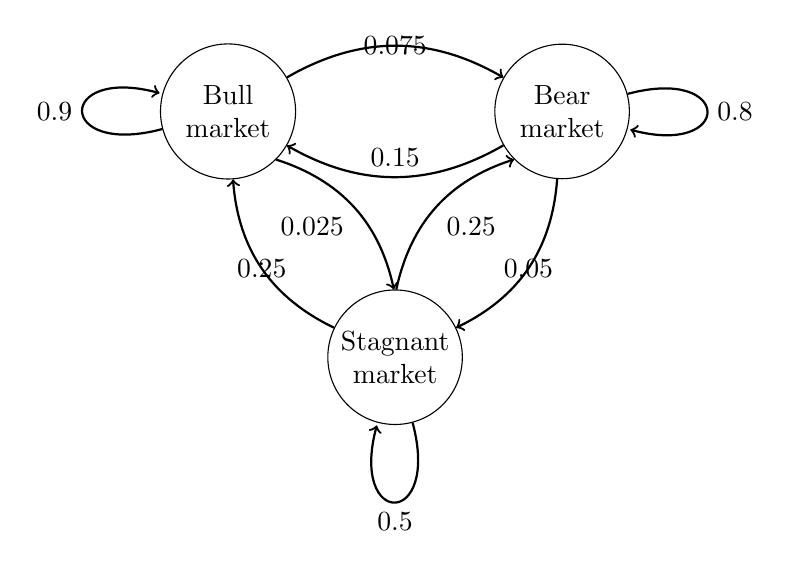
\begin{tikzpicture}[scale=.1] \tikzstyle{node} = [circle, draw,text width=4.5em, text badly centered, node distance=3cm, inner sep=0pt] \node [node] (node0) {Stagnant market}; \node [node,above left of=node0,yshift=1cm] (node1) {Bull market}; \node [node,above right of=node0,yshift=1cm] (node2) {Bear market}; \path (node0) edge [bend left,->,thick] node [pos=0.5] { 0.25} (node1); \path (node1.south east) edge [bend left,->,thick] node [pos=0.5,below left] { 0.025} (node0); \path (node1) edge [bend left,->,thick] node [pos=0.5] { 0.075} (node2); \path (node2) edge [bend left,->,thick] node [pos=0.5] { 0.05} (node0); \path (node2) edge [bend left,->,thick] node [above,pos=0.5] {0.15} (node1); \path (node2.south west) edge [bend right,<-,thick] node [pos=0.5,below right] {0.25} (node0); \path (node0) edge [loop below,->,thick] node [pos=0.5] {0.5} (node0); \path (node1) edge [loop left,->,thick] node [pos=0.5] {0.9} (node1); \path (node2) edge [loop right,->,thick] node [pos=0.5] {0.8} (node2); \end{tikzpicture}}
\par\end{center}%
\end{minipage}\hfill{}%
\begin{minipage}[t]{0.45\columnwidth}%
\noindent \begin{center}
\begin{tabular}{c|c|c|c}
 & Bull & Bear & Stag.\tabularnewline
\hline 
Bull & 0.9 & 0.075 & 0.025\tabularnewline
\hline 
Bear & 0.15 & 0.8 & 0.05\tabularnewline
\hline 
Stag. & 0.25 & 0.25 & 0.5\tabularnewline
\end{tabular}
\par\end{center}

%
\end{minipage}
\end{figure}

\item {\footnotesize{}Hidden Markov models (hierarchical model) great for
speech recognition}{\footnotesize \par}
\end{itemize}

\lyxframeend{}\lyxframe{}
\begin{block}
{Definition} {\scriptsize{}A random variable $N$ is distributed
Poisson$\left(\lambda\right)$ on some unit interval $u$ if at 
\[
P\left(N=n\text{ events in interval}\right)=\frac{\lambda^{n}e^{-\lambda}}{n!}
\]
$\lambda$ is called the rate parameter.}{\scriptsize \par}\end{block}
\begin{itemize}
\item {\scriptsize{}Intuitively ``time'' between events is exponentially
distributed but independent}{\scriptsize \par}
\item {\scriptsize{}Phone calls at an exchange, arrivals bank queue, train
arrivals (on a bad day!)}{\scriptsize \par}\end{itemize}
\begin{exampleblock}
{Example} {\scriptsize{}A }\emph{\scriptsize{}Poisson process }{\scriptsize{}$N_{t}$
on $\left[0,\infty\right)$ with rate $\lambda$ is a stochastic process
where the number of events in any interval of length $t$ is distributed
Poisson$\left(\lambda t\right)$.}{\scriptsize \par}
\end{exampleblock}


\begin{figure}

\begin{algorithmic}[1]
lambda <- 1 \\
x1 <- cumsum(rexp(50),rate=lambda) \\
y1 <- cumsum(c(0,rep(1,50))) \\
plot(stepfun(x1,y1),xlim = c(0,50),do.points = F)
\end{algorithmic} 

\end{figure}



\lyxframeend{}\lyxframe{}

\begin{figure}
\scalebox{0.7}{
 \begin{tikzpicture}[x=1pt,y=1pt] \definecolor{fillColor}{RGB}{255,255,255} \path[use as bounding box,fill=fillColor,fill opacity=0.00] (0,0) rectangle (361.35,361.35); \begin{scope} \path[clip] (  0.00,  0.00) rectangle (361.35,361.35); \definecolor{drawColor}{RGB}{0,0,0}
\path[draw=drawColor,line width= 0.4pt,line join=round,line cap=round] ( 59.83, 61.20) -- (325.52, 61.20);
\path[draw=drawColor,line width= 0.4pt,line join=round,line cap=round] ( 59.83, 61.20) -- ( 59.83, 55.20);
\path[draw=drawColor,line width= 0.4pt,line join=round,line cap=round] (112.97, 61.20) -- (112.97, 55.20);
\path[draw=drawColor,line width= 0.4pt,line join=round,line cap=round] (166.11, 61.20) -- (166.11, 55.20);
\path[draw=drawColor,line width= 0.4pt,line join=round,line cap=round] (219.24, 61.20) -- (219.24, 55.20);
\path[draw=drawColor,line width= 0.4pt,line join=round,line cap=round] (272.38, 61.20) -- (272.38, 55.20);
\path[draw=drawColor,line width= 0.4pt,line join=round,line cap=round] (325.52, 61.20) -- (325.52, 55.20);
\node[text=drawColor,anchor=base,inner sep=0pt, outer sep=0pt, scale=  1.00] at ( 59.83, 39.60) {0};
\node[text=drawColor,anchor=base,inner sep=0pt, outer sep=0pt, scale=  1.00] at (112.97, 39.60) {10};
\node[text=drawColor,anchor=base,inner sep=0pt, outer sep=0pt, scale=  1.00] at (166.11, 39.60) {20};
\node[text=drawColor,anchor=base,inner sep=0pt, outer sep=0pt, scale=  1.00] at (219.24, 39.60) {30};
\node[text=drawColor,anchor=base,inner sep=0pt, outer sep=0pt, scale=  1.00] at (272.38, 39.60) {40};
\node[text=drawColor,anchor=base,inner sep=0pt, outer sep=0pt, scale=  1.00] at (325.52, 39.60) {50};
\path[draw=drawColor,line width= 0.4pt,line join=round,line cap=round] ( 49.20, 70.49) -- ( 49.20,302.86);
\path[draw=drawColor,line width= 0.4pt,line join=round,line cap=round] ( 49.20, 70.49) -- ( 43.20, 70.49);
\path[draw=drawColor,line width= 0.4pt,line join=round,line cap=round] ( 49.20,116.97) -- ( 43.20,116.97);
\path[draw=drawColor,line width= 0.4pt,line join=round,line cap=round] ( 49.20,163.44) -- ( 43.20,163.44);
\path[draw=drawColor,line width= 0.4pt,line join=round,line cap=round] ( 49.20,209.91) -- ( 43.20,209.91);
\path[draw=drawColor,line width= 0.4pt,line join=round,line cap=round] ( 49.20,256.38) -- ( 43.20,256.38);
\path[draw=drawColor,line width= 0.4pt,line join=round,line cap=round] ( 49.20,302.86) -- ( 43.20,302.86);
\node[text=drawColor,rotate= 90.00,anchor=base,inner sep=0pt, outer sep=0pt, scale=  1.00] at ( 34.80, 70.49) {0};
\node[text=drawColor,rotate= 90.00,anchor=base,inner sep=0pt, outer sep=0pt, scale=  1.00] at ( 34.80,116.97) {10};
\node[text=drawColor,rotate= 90.00,anchor=base,inner sep=0pt, outer sep=0pt, scale=  1.00] at ( 34.80,163.44) {20};
\node[text=drawColor,rotate= 90.00,anchor=base,inner sep=0pt, outer sep=0pt, scale=  1.00] at ( 34.80,209.91) {30};
\node[text=drawColor,rotate= 90.00,anchor=base,inner sep=0pt, outer sep=0pt, scale=  1.00] at ( 34.80,256.38) {40};
\node[text=drawColor,rotate= 90.00,anchor=base,inner sep=0pt, outer sep=0pt, scale=  1.00] at ( 34.80,302.86) {50};
\path[draw=drawColor,line width= 0.4pt,line join=round,line cap=round] ( 49.20, 61.20) -- 	(336.15, 61.20) -- 	(336.15,312.15) -- 	( 49.20,312.15) -- 	( 49.20, 61.20); \end{scope} \begin{scope} \path[clip] (  0.00,  0.00) rectangle (361.35,361.35); \definecolor{drawColor}{RGB}{0,0,0}
\node[text=drawColor,anchor=base,inner sep=0pt, outer sep=0pt, scale=  1.00] at (192.68, 15.60) {time};
\node[text=drawColor,rotate= 90.00,anchor=base,inner sep=0pt, outer sep=0pt, scale=  1.00] at ( 10.80,186.67) {arrivals}; \end{scope} \begin{scope} \path[clip] ( 49.20, 61.20) rectangle (336.15,312.15); \definecolor{drawColor}{RGB}{255,0,0}
\path[draw=drawColor,line width= 0.4pt,line join=round,line cap=round] (  0.00, 70.49) -- ( 74.21, 70.49);
\path[draw=drawColor,line width= 0.4pt,line join=round,line cap=round] ( 74.21, 75.14) -- ( 84.09, 75.14);
\path[draw=drawColor,line width= 0.4pt,line join=round,line cap=round] ( 84.09, 79.79) -- ( 88.94, 79.79);
\path[draw=drawColor,line width= 0.4pt,line join=round,line cap=round] ( 88.94, 84.44) -- (123.65, 84.44);
\path[draw=drawColor,line width= 0.4pt,line join=round,line cap=round] (123.65, 89.08) -- (161.19, 89.08);
\path[draw=drawColor,line width= 0.4pt,line join=round,line cap=round] (161.19, 93.73) -- (178.21, 93.73);
\path[draw=drawColor,line width= 0.4pt,line join=round,line cap=round] (178.21, 98.38) -- (189.72, 98.38);
\path[draw=drawColor,line width= 0.4pt,line join=round,line cap=round] (189.72,103.02) -- (205.04,103.02);
\path[draw=drawColor,line width= 0.4pt,line join=round,line cap=round] (205.04,107.67) -- (301.70,107.67);
\path[draw=drawColor,line width= 0.4pt,line join=round,line cap=round] (301.70,112.32) -- (349.06,112.32);
\path[draw=drawColor,line width= 0.4pt,line join=round,line cap=round] (349.06,116.97) -- (354.30,116.97);
\path[draw=drawColor,line width= 0.4pt,line join=round,line cap=round] (354.30,121.61) -- (361.35,121.61);
\path[draw=drawColor,line width= 0.4pt,line join=round,line cap=round] ( 74.21, 70.49) -- ( 74.21, 75.14);
\path[draw=drawColor,line width= 0.4pt,line join=round,line cap=round] ( 84.09, 75.14) -- ( 84.09, 79.79);
\path[draw=drawColor,line width= 0.4pt,line join=round,line cap=round] ( 88.94, 79.79) -- ( 88.94, 84.44);
\path[draw=drawColor,line width= 0.4pt,line join=round,line cap=round] (123.65, 84.44) -- (123.65, 89.08);
\path[draw=drawColor,line width= 0.4pt,line join=round,line cap=round] (161.19, 89.08) -- (161.19, 93.73);
\path[draw=drawColor,line width= 0.4pt,line join=round,line cap=round] (178.21, 93.73) -- (178.21, 98.38);
\path[draw=drawColor,line width= 0.4pt,line join=round,line cap=round] (189.72, 98.38) -- (189.72,103.02);
\path[draw=drawColor,line width= 0.4pt,line join=round,line cap=round] (205.04,103.02) -- (205.04,107.67);
\path[draw=drawColor,line width= 0.4pt,line join=round,line cap=round] (301.70,107.67) -- (301.70,112.32);
\path[draw=drawColor,line width= 0.4pt,line join=round,line cap=round] (349.06,112.32) -- (349.06,116.97);
\path[draw=drawColor,line width= 0.4pt,line join=round,line cap=round] (354.30,116.97) -- (354.30,121.61); \end{scope} \begin{scope} \path[clip] (  0.00,  0.00) rectangle (361.35,361.35); \definecolor{drawColor}{RGB}{0,0,0}
\path[draw=drawColor,line width= 0.4pt,line join=round,line cap=round] ( 59.83, 61.20) -- (325.52, 61.20);
\path[draw=drawColor,line width= 0.4pt,line join=round,line cap=round] ( 59.83, 61.20) -- ( 59.83, 55.20);
\path[draw=drawColor,line width= 0.4pt,line join=round,line cap=round] (112.97, 61.20) -- (112.97, 55.20);
\path[draw=drawColor,line width= 0.4pt,line join=round,line cap=round] (166.11, 61.20) -- (166.11, 55.20);
\path[draw=drawColor,line width= 0.4pt,line join=round,line cap=round] (219.24, 61.20) -- (219.24, 55.20);
\path[draw=drawColor,line width= 0.4pt,line join=round,line cap=round] (272.38, 61.20) -- (272.38, 55.20);
\path[draw=drawColor,line width= 0.4pt,line join=round,line cap=round] (325.52, 61.20) -- (325.52, 55.20);
\node[text=drawColor,anchor=base,inner sep=0pt, outer sep=0pt, scale=  1.00] at ( 59.83, 39.60) {0};
\node[text=drawColor,anchor=base,inner sep=0pt, outer sep=0pt, scale=  1.00] at (112.97, 39.60) {10};
\node[text=drawColor,anchor=base,inner sep=0pt, outer sep=0pt, scale=  1.00] at (166.11, 39.60) {20};
\node[text=drawColor,anchor=base,inner sep=0pt, outer sep=0pt, scale=  1.00] at (219.24, 39.60) {30};
\node[text=drawColor,anchor=base,inner sep=0pt, outer sep=0pt, scale=  1.00] at (272.38, 39.60) {40};
\node[text=drawColor,anchor=base,inner sep=0pt, outer sep=0pt, scale=  1.00] at (325.52, 39.60) {50};
\path[draw=drawColor,line width= 0.4pt,line join=round,line cap=round] ( 49.20, 70.49) -- ( 49.20,302.86);
\path[draw=drawColor,line width= 0.4pt,line join=round,line cap=round] ( 49.20, 70.49) -- ( 43.20, 70.49);
\path[draw=drawColor,line width= 0.4pt,line join=round,line cap=round] ( 49.20,116.97) -- ( 43.20,116.97);
\path[draw=drawColor,line width= 0.4pt,line join=round,line cap=round] ( 49.20,163.44) -- ( 43.20,163.44);
\path[draw=drawColor,line width= 0.4pt,line join=round,line cap=round] ( 49.20,209.91) -- ( 43.20,209.91);
\path[draw=drawColor,line width= 0.4pt,line join=round,line cap=round] ( 49.20,256.38) -- ( 43.20,256.38);
\path[draw=drawColor,line width= 0.4pt,line join=round,line cap=round] ( 49.20,302.86) -- ( 43.20,302.86);
\node[text=drawColor,rotate= 90.00,anchor=base,inner sep=0pt, outer sep=0pt, scale=  1.00] at ( 34.80, 70.49) {0};
\node[text=drawColor,rotate= 90.00,anchor=base,inner sep=0pt, outer sep=0pt, scale=  1.00] at ( 34.80,116.97) {10};
\node[text=drawColor,rotate= 90.00,anchor=base,inner sep=0pt, outer sep=0pt, scale=  1.00] at ( 34.80,163.44) {20};
\node[text=drawColor,rotate= 90.00,anchor=base,inner sep=0pt, outer sep=0pt, scale=  1.00] at ( 34.80,209.91) {30};
\node[text=drawColor,rotate= 90.00,anchor=base,inner sep=0pt, outer sep=0pt, scale=  1.00] at ( 34.80,256.38) {40};
\node[text=drawColor,rotate= 90.00,anchor=base,inner sep=0pt, outer sep=0pt, scale=  1.00] at ( 34.80,302.86) {50};
\path[draw=drawColor,line width= 0.4pt,line join=round,line cap=round] ( 49.20, 61.20) -- 	(336.15, 61.20) -- 	(336.15,312.15) -- 	( 49.20,312.15) -- 	( 49.20, 61.20); \end{scope} \begin{scope} \path[clip] ( 49.20, 61.20) rectangle (336.15,312.15); \definecolor{drawColor}{RGB}{0,255,0}
\path[draw=drawColor,line width= 0.4pt,line join=round,line cap=round] (  0.00, 70.49) -- ( 71.86, 70.49);
\path[draw=drawColor,line width= 0.4pt,line join=round,line cap=round] ( 71.86, 75.14) -- ( 74.60, 75.14);
\path[draw=drawColor,line width= 0.4pt,line join=round,line cap=round] ( 74.60, 79.79) -- ( 75.18, 79.79);
\path[draw=drawColor,line width= 0.4pt,line join=round,line cap=round] ( 75.18, 84.44) -- ( 93.77, 84.44);
\path[draw=drawColor,line width= 0.4pt,line join=round,line cap=round] ( 93.77, 89.08) -- ( 94.59, 89.08);
\path[draw=drawColor,line width= 0.4pt,line join=round,line cap=round] ( 94.59, 93.73) -- (120.70, 93.73);
\path[draw=drawColor,line width= 0.4pt,line join=round,line cap=round] (120.70, 98.38) -- (136.90, 98.38);
\path[draw=drawColor,line width= 0.4pt,line join=round,line cap=round] (136.90,103.02) -- (151.57,103.02);
\path[draw=drawColor,line width= 0.4pt,line join=round,line cap=round] (151.57,107.67) -- (153.32,107.67);
\path[draw=drawColor,line width= 0.4pt,line join=round,line cap=round] (153.32,112.32) -- (157.88,112.32);
\path[draw=drawColor,line width= 0.4pt,line join=round,line cap=round] (157.88,116.97) -- (166.49,116.97);
\path[draw=drawColor,line width= 0.4pt,line join=round,line cap=round] (166.49,121.61) -- (169.07,121.61);
\path[draw=drawColor,line width= 0.4pt,line join=round,line cap=round] (169.07,126.26) -- (173.80,126.26);
\path[draw=drawColor,line width= 0.4pt,line join=round,line cap=round] (173.80,130.91) -- (194.08,130.91);
\path[draw=drawColor,line width= 0.4pt,line join=round,line cap=round] (194.08,135.56) -- (195.54,135.56);
\path[draw=drawColor,line width= 0.4pt,line join=round,line cap=round] (195.54,140.20) -- (199.19,140.20);
\path[draw=drawColor,line width= 0.4pt,line join=round,line cap=round] (199.19,144.85) -- (201.58,144.85);
\path[draw=drawColor,line width= 0.4pt,line join=round,line cap=round] (201.58,149.50) -- (256.10,149.50);
\path[draw=drawColor,line width= 0.4pt,line join=round,line cap=round] (256.10,154.14) -- (268.58,154.14);
\path[draw=drawColor,line width= 0.4pt,line join=round,line cap=round] (268.58,158.79) -- (271.50,158.79);
\path[draw=drawColor,line width= 0.4pt,line join=round,line cap=round] (271.50,163.44) -- (273.83,163.44);
\path[draw=drawColor,line width= 0.4pt,line join=round,line cap=round] (273.83,168.09) -- (280.60,168.09);
\path[draw=drawColor,line width= 0.4pt,line join=round,line cap=round] (280.60,172.73) -- (304.18,172.73);
\path[draw=drawColor,line width= 0.4pt,line join=round,line cap=round] (304.18,177.38) -- (306.03,177.38);
\path[draw=drawColor,line width= 0.4pt,line join=round,line cap=round] (306.03,182.03) -- (310.17,182.03);
\path[draw=drawColor,line width= 0.4pt,line join=round,line cap=round] (310.17,186.67) -- (310.78,186.67);
\path[draw=drawColor,line width= 0.4pt,line join=round,line cap=round] (310.78,191.32) -- (323.22,191.32);
\path[draw=drawColor,line width= 0.4pt,line join=round,line cap=round] (323.22,195.97) -- (327.44,195.97);
\path[draw=drawColor,line width= 0.4pt,line join=round,line cap=round] (327.44,200.62) -- (336.51,200.62);
\path[draw=drawColor,line width= 0.4pt,line join=round,line cap=round] (336.51,205.26) -- (361.35,205.26);
\path[draw=drawColor,line width= 0.4pt,line join=round,line cap=round] ( 71.86, 70.49) -- ( 71.86, 75.14);
\path[draw=drawColor,line width= 0.4pt,line join=round,line cap=round] ( 74.60, 75.14) -- ( 74.60, 79.79);
\path[draw=drawColor,line width= 0.4pt,line join=round,line cap=round] ( 75.18, 79.79) -- ( 75.18, 84.44);
\path[draw=drawColor,line width= 0.4pt,line join=round,line cap=round] ( 93.77, 84.44) -- ( 93.77, 89.08);
\path[draw=drawColor,line width= 0.4pt,line join=round,line cap=round] ( 94.59, 89.08) -- ( 94.59, 93.73);
\path[draw=drawColor,line width= 0.4pt,line join=round,line cap=round] (120.70, 93.73) -- (120.70, 98.38);
\path[draw=drawColor,line width= 0.4pt,line join=round,line cap=round] (136.90, 98.38) -- (136.90,103.02);
\path[draw=drawColor,line width= 0.4pt,line join=round,line cap=round] (151.57,103.02) -- (151.57,107.67);
\path[draw=drawColor,line width= 0.4pt,line join=round,line cap=round] (153.32,107.67) -- (153.32,112.32);
\path[draw=drawColor,line width= 0.4pt,line join=round,line cap=round] (157.88,112.32) -- (157.88,116.97);
\path[draw=drawColor,line width= 0.4pt,line join=round,line cap=round] (166.49,116.97) -- (166.49,121.61);
\path[draw=drawColor,line width= 0.4pt,line join=round,line cap=round] (169.07,121.61) -- (169.07,126.26);
\path[draw=drawColor,line width= 0.4pt,line join=round,line cap=round] (173.80,126.26) -- (173.80,130.91);
\path[draw=drawColor,line width= 0.4pt,line join=round,line cap=round] (194.08,130.91) -- (194.08,135.56);
\path[draw=drawColor,line width= 0.4pt,line join=round,line cap=round] (195.54,135.56) -- (195.54,140.20);
\path[draw=drawColor,line width= 0.4pt,line join=round,line cap=round] (199.19,140.20) -- (199.19,144.85);
\path[draw=drawColor,line width= 0.4pt,line join=round,line cap=round] (201.58,144.85) -- (201.58,149.50);
\path[draw=drawColor,line width= 0.4pt,line join=round,line cap=round] (256.10,149.50) -- (256.10,154.14);
\path[draw=drawColor,line width= 0.4pt,line join=round,line cap=round] (268.58,154.14) -- (268.58,158.79);
\path[draw=drawColor,line width= 0.4pt,line join=round,line cap=round] (271.50,158.79) -- (271.50,163.44);
\path[draw=drawColor,line width= 0.4pt,line join=round,line cap=round] (273.83,163.44) -- (273.83,168.09);
\path[draw=drawColor,line width= 0.4pt,line join=round,line cap=round] (280.60,168.09) -- (280.60,172.73);
\path[draw=drawColor,line width= 0.4pt,line join=round,line cap=round] (304.18,172.73) -- (304.18,177.38);
\path[draw=drawColor,line width= 0.4pt,line join=round,line cap=round] (306.03,177.38) -- (306.03,182.03);
\path[draw=drawColor,line width= 0.4pt,line join=round,line cap=round] (310.17,182.03) -- (310.17,186.67);
\path[draw=drawColor,line width= 0.4pt,line join=round,line cap=round] (310.78,186.67) -- (310.78,191.32);
\path[draw=drawColor,line width= 0.4pt,line join=round,line cap=round] (323.22,191.32) -- (323.22,195.97);
\path[draw=drawColor,line width= 0.4pt,line join=round,line cap=round] (327.44,195.97) -- (327.44,200.62);
\path[draw=drawColor,line width= 0.4pt,line join=round,line cap=round] (336.51,200.62) -- (336.51,205.26); \end{scope} \begin{scope} \path[clip] (  0.00,  0.00) rectangle (361.35,361.35); \definecolor{drawColor}{RGB}{0,0,0}
\path[draw=drawColor,line width= 0.4pt,line join=round,line cap=round] ( 59.83, 61.20) -- (325.52, 61.20);
\path[draw=drawColor,line width= 0.4pt,line join=round,line cap=round] ( 59.83, 61.20) -- ( 59.83, 55.20);
\path[draw=drawColor,line width= 0.4pt,line join=round,line cap=round] (112.97, 61.20) -- (112.97, 55.20);
\path[draw=drawColor,line width= 0.4pt,line join=round,line cap=round] (166.11, 61.20) -- (166.11, 55.20);
\path[draw=drawColor,line width= 0.4pt,line join=round,line cap=round] (219.24, 61.20) -- (219.24, 55.20);
\path[draw=drawColor,line width= 0.4pt,line join=round,line cap=round] (272.38, 61.20) -- (272.38, 55.20);
\path[draw=drawColor,line width= 0.4pt,line join=round,line cap=round] (325.52, 61.20) -- (325.52, 55.20);
\node[text=drawColor,anchor=base,inner sep=0pt, outer sep=0pt, scale=  1.00] at ( 59.83, 39.60) {0};
\node[text=drawColor,anchor=base,inner sep=0pt, outer sep=0pt, scale=  1.00] at (112.97, 39.60) {10};
\node[text=drawColor,anchor=base,inner sep=0pt, outer sep=0pt, scale=  1.00] at (166.11, 39.60) {20};
\node[text=drawColor,anchor=base,inner sep=0pt, outer sep=0pt, scale=  1.00] at (219.24, 39.60) {30};
\node[text=drawColor,anchor=base,inner sep=0pt, outer sep=0pt, scale=  1.00] at (272.38, 39.60) {40};
\node[text=drawColor,anchor=base,inner sep=0pt, outer sep=0pt, scale=  1.00] at (325.52, 39.60) {50};
\path[draw=drawColor,line width= 0.4pt,line join=round,line cap=round] ( 49.20, 70.49) -- ( 49.20,302.86);
\path[draw=drawColor,line width= 0.4pt,line join=round,line cap=round] ( 49.20, 70.49) -- ( 43.20, 70.49);
\path[draw=drawColor,line width= 0.4pt,line join=round,line cap=round] ( 49.20,116.97) -- ( 43.20,116.97);
\path[draw=drawColor,line width= 0.4pt,line join=round,line cap=round] ( 49.20,163.44) -- ( 43.20,163.44);
\path[draw=drawColor,line width= 0.4pt,line join=round,line cap=round] ( 49.20,209.91) -- ( 43.20,209.91);
\path[draw=drawColor,line width= 0.4pt,line join=round,line cap=round] ( 49.20,256.38) -- ( 43.20,256.38);
\path[draw=drawColor,line width= 0.4pt,line join=round,line cap=round] ( 49.20,302.86) -- ( 43.20,302.86);
\node[text=drawColor,rotate= 90.00,anchor=base,inner sep=0pt, outer sep=0pt, scale=  1.00] at ( 34.80, 70.49) {0};
\node[text=drawColor,rotate= 90.00,anchor=base,inner sep=0pt, outer sep=0pt, scale=  1.00] at ( 34.80,116.97) {10};
\node[text=drawColor,rotate= 90.00,anchor=base,inner sep=0pt, outer sep=0pt, scale=  1.00] at ( 34.80,163.44) {20};
\node[text=drawColor,rotate= 90.00,anchor=base,inner sep=0pt, outer sep=0pt, scale=  1.00] at ( 34.80,209.91) {30};
\node[text=drawColor,rotate= 90.00,anchor=base,inner sep=0pt, outer sep=0pt, scale=  1.00] at ( 34.80,256.38) {40};
\node[text=drawColor,rotate= 90.00,anchor=base,inner sep=0pt, outer sep=0pt, scale=  1.00] at ( 34.80,302.86) {50};
\path[draw=drawColor,line width= 0.4pt,line join=round,line cap=round] ( 49.20, 61.20) -- 	(336.15, 61.20) -- 	(336.15,312.15) -- 	( 49.20,312.15) -- 	( 49.20, 61.20); \end{scope} \begin{scope} \path[clip] ( 49.20, 61.20) rectangle (336.15,312.15); \definecolor{drawColor}{RGB}{0,0,255}
\path[draw=drawColor,line width= 0.4pt,line join=round,line cap=round] (  0.00, 70.49) -- ( 63.65, 70.49);
\path[draw=drawColor,line width= 0.4pt,line join=round,line cap=round] ( 63.65, 75.14) -- ( 72.57, 75.14);
\path[draw=drawColor,line width= 0.4pt,line join=round,line cap=round] ( 72.57, 79.79) -- ( 74.84, 79.79);
\path[draw=drawColor,line width= 0.4pt,line join=round,line cap=round] ( 74.84, 84.44) -- ( 83.99, 84.44);
\path[draw=drawColor,line width= 0.4pt,line join=round,line cap=round] ( 83.99, 89.08) -- ( 87.94, 89.08);
\path[draw=drawColor,line width= 0.4pt,line join=round,line cap=round] ( 87.94, 93.73) -- ( 93.11, 93.73);
\path[draw=drawColor,line width= 0.4pt,line join=round,line cap=round] ( 93.11, 98.38) -- ( 94.86, 98.38);
\path[draw=drawColor,line width= 0.4pt,line join=round,line cap=round] ( 94.86,103.02) -- ( 97.28,103.02);
\path[draw=drawColor,line width= 0.4pt,line join=round,line cap=round] ( 97.28,107.67) -- ( 98.04,107.67);
\path[draw=drawColor,line width= 0.4pt,line join=round,line cap=round] ( 98.04,112.32) -- ( 98.80,112.32);
\path[draw=drawColor,line width= 0.4pt,line join=round,line cap=round] ( 98.80,116.97) -- (103.39,116.97);
\path[draw=drawColor,line width= 0.4pt,line join=round,line cap=round] (103.39,121.61) -- (103.45,121.61);
\path[draw=drawColor,line width= 0.4pt,line join=round,line cap=round] (103.45,126.26) -- (103.48,126.26);
\path[draw=drawColor,line width= 0.4pt,line join=round,line cap=round] (103.48,130.91) -- (103.99,130.91);
\path[draw=drawColor,line width= 0.4pt,line join=round,line cap=round] (103.99,135.56) -- (104.65,135.56);
\path[draw=drawColor,line width= 0.4pt,line join=round,line cap=round] (104.65,140.20) -- (107.78,140.20);
\path[draw=drawColor,line width= 0.4pt,line join=round,line cap=round] (107.78,144.85) -- (118.08,144.85);
\path[draw=drawColor,line width= 0.4pt,line join=round,line cap=round] (118.08,149.50) -- (120.31,149.50);
\path[draw=drawColor,line width= 0.4pt,line join=round,line cap=round] (120.31,154.14) -- (121.01,154.14);
\path[draw=drawColor,line width= 0.4pt,line join=round,line cap=round] (121.01,158.79) -- (144.68,158.79);
\path[draw=drawColor,line width= 0.4pt,line join=round,line cap=round] (144.68,163.44) -- (148.51,163.44);
\path[draw=drawColor,line width= 0.4pt,line join=round,line cap=round] (148.51,168.09) -- (155.61,168.09);
\path[draw=drawColor,line width= 0.4pt,line join=round,line cap=round] (155.61,172.73) -- (166.59,172.73);
\path[draw=drawColor,line width= 0.4pt,line join=round,line cap=round] (166.59,177.38) -- (167.07,177.38);
\path[draw=drawColor,line width= 0.4pt,line join=round,line cap=round] (167.07,182.03) -- (168.61,182.03);
\path[draw=drawColor,line width= 0.4pt,line join=round,line cap=round] (168.61,186.67) -- (170.86,186.67);
\path[draw=drawColor,line width= 0.4pt,line join=round,line cap=round] (170.86,191.32) -- (181.18,191.32);
\path[draw=drawColor,line width= 0.4pt,line join=round,line cap=round] (181.18,195.97) -- (186.19,195.97);
\path[draw=drawColor,line width= 0.4pt,line join=round,line cap=round] (186.19,200.62) -- (195.98,200.62);
\path[draw=drawColor,line width= 0.4pt,line join=round,line cap=round] (195.98,205.26) -- (202.15,205.26);
\path[draw=drawColor,line width= 0.4pt,line join=round,line cap=round] (202.15,209.91) -- (211.07,209.91);
\path[draw=drawColor,line width= 0.4pt,line join=round,line cap=round] (211.07,214.56) -- (236.08,214.56);
\path[draw=drawColor,line width= 0.4pt,line join=round,line cap=round] (236.08,219.21) -- (236.45,219.21);
\path[draw=drawColor,line width= 0.4pt,line join=round,line cap=round] (236.45,223.85) -- (241.38,223.85);
\path[draw=drawColor,line width= 0.4pt,line join=round,line cap=round] (241.38,228.50) -- (242.23,228.50);
\path[draw=drawColor,line width= 0.4pt,line join=round,line cap=round] (242.23,233.15) -- (245.73,233.15);
\path[draw=drawColor,line width= 0.4pt,line join=round,line cap=round] (245.73,237.79) -- (251.22,237.79);
\path[draw=drawColor,line width= 0.4pt,line join=round,line cap=round] (251.22,242.44) -- (257.70,242.44);
\path[draw=drawColor,line width= 0.4pt,line join=round,line cap=round] (257.70,247.09) -- (258.83,247.09);
\path[draw=drawColor,line width= 0.4pt,line join=round,line cap=round] (258.83,251.74) -- (262.91,251.74);
\path[draw=drawColor,line width= 0.4pt,line join=round,line cap=round] (262.91,256.38) -- (265.57,256.38);
\path[draw=drawColor,line width= 0.4pt,line join=round,line cap=round] (265.57,261.03) -- (268.72,261.03);
\path[draw=drawColor,line width= 0.4pt,line join=round,line cap=round] (268.72,265.68) -- (275.39,265.68);
\path[draw=drawColor,line width= 0.4pt,line join=round,line cap=round] (275.39,270.32) -- (297.74,270.32);
\path[draw=drawColor,line width= 0.4pt,line join=round,line cap=round] (297.74,274.97) -- (298.08,274.97);
\path[draw=drawColor,line width= 0.4pt,line join=round,line cap=round] (298.08,279.62) -- (309.34,279.62);
\path[draw=drawColor,line width= 0.4pt,line join=round,line cap=round] (309.34,284.27) -- (311.07,284.27);
\path[draw=drawColor,line width= 0.4pt,line join=round,line cap=round] (311.07,288.91) -- (318.49,288.91);
\path[draw=drawColor,line width= 0.4pt,line join=round,line cap=round] (318.49,293.56) -- (322.03,293.56);
\path[draw=drawColor,line width= 0.4pt,line join=round,line cap=round] (322.03,298.21) -- (325.97,298.21);
\path[draw=drawColor,line width= 0.4pt,line join=round,line cap=round] (325.97,302.86) -- (361.35,302.86);
\path[draw=drawColor,line width= 0.4pt,line join=round,line cap=round] ( 63.65, 70.49) -- ( 63.65, 75.14);
\path[draw=drawColor,line width= 0.4pt,line join=round,line cap=round] ( 72.57, 75.14) -- ( 72.57, 79.79);
\path[draw=drawColor,line width= 0.4pt,line join=round,line cap=round] ( 74.84, 79.79) -- ( 74.84, 84.44);
\path[draw=drawColor,line width= 0.4pt,line join=round,line cap=round] ( 83.99, 84.44) -- ( 83.99, 89.08);
\path[draw=drawColor,line width= 0.4pt,line join=round,line cap=round] ( 87.94, 89.08) -- ( 87.94, 93.73);
\path[draw=drawColor,line width= 0.4pt,line join=round,line cap=round] ( 93.11, 93.73) -- ( 93.11, 98.38);
\path[draw=drawColor,line width= 0.4pt,line join=round,line cap=round] ( 94.86, 98.38) -- ( 94.86,103.02);
\path[draw=drawColor,line width= 0.4pt,line join=round,line cap=round] ( 97.28,103.02) -- ( 97.28,107.67);
\path[draw=drawColor,line width= 0.4pt,line join=round,line cap=round] ( 98.04,107.67) -- ( 98.04,112.32);
\path[draw=drawColor,line width= 0.4pt,line join=round,line cap=round] ( 98.80,112.32) -- ( 98.80,116.97);
\path[draw=drawColor,line width= 0.4pt,line join=round,line cap=round] (103.39,116.97) -- (103.39,121.61);
\path[draw=drawColor,line width= 0.4pt,line join=round,line cap=round] (103.45,121.61) -- (103.45,126.26);
\path[draw=drawColor,line width= 0.4pt,line join=round,line cap=round] (103.48,126.26) -- (103.48,130.91);
\path[draw=drawColor,line width= 0.4pt,line join=round,line cap=round] (103.99,130.91) -- (103.99,135.56);
\path[draw=drawColor,line width= 0.4pt,line join=round,line cap=round] (104.65,135.56) -- (104.65,140.20);
\path[draw=drawColor,line width= 0.4pt,line join=round,line cap=round] (107.78,140.20) -- (107.78,144.85);
\path[draw=drawColor,line width= 0.4pt,line join=round,line cap=round] (118.08,144.85) -- (118.08,149.50);
\path[draw=drawColor,line width= 0.4pt,line join=round,line cap=round] (120.31,149.50) -- (120.31,154.14);
\path[draw=drawColor,line width= 0.4pt,line join=round,line cap=round] (121.01,154.14) -- (121.01,158.79);
\path[draw=drawColor,line width= 0.4pt,line join=round,line cap=round] (144.68,158.79) -- (144.68,163.44);
\path[draw=drawColor,line width= 0.4pt,line join=round,line cap=round] (148.51,163.44) -- (148.51,168.09);
\path[draw=drawColor,line width= 0.4pt,line join=round,line cap=round] (155.61,168.09) -- (155.61,172.73);
\path[draw=drawColor,line width= 0.4pt,line join=round,line cap=round] (166.59,172.73) -- (166.59,177.38);
\path[draw=drawColor,line width= 0.4pt,line join=round,line cap=round] (167.07,177.38) -- (167.07,182.03);
\path[draw=drawColor,line width= 0.4pt,line join=round,line cap=round] (168.61,182.03) -- (168.61,186.67);
\path[draw=drawColor,line width= 0.4pt,line join=round,line cap=round] (170.86,186.67) -- (170.86,191.32);
\path[draw=drawColor,line width= 0.4pt,line join=round,line cap=round] (181.18,191.32) -- (181.18,195.97);
\path[draw=drawColor,line width= 0.4pt,line join=round,line cap=round] (186.19,195.97) -- (186.19,200.62);
\path[draw=drawColor,line width= 0.4pt,line join=round,line cap=round] (195.98,200.62) -- (195.98,205.26);
\path[draw=drawColor,line width= 0.4pt,line join=round,line cap=round] (202.15,205.26) -- (202.15,209.91);
\path[draw=drawColor,line width= 0.4pt,line join=round,line cap=round] (211.07,209.91) -- (211.07,214.56);
\path[draw=drawColor,line width= 0.4pt,line join=round,line cap=round] (236.08,214.56) -- (236.08,219.21);
\path[draw=drawColor,line width= 0.4pt,line join=round,line cap=round] (236.45,219.21) -- (236.45,223.85);
\path[draw=drawColor,line width= 0.4pt,line join=round,line cap=round] (241.38,223.85) -- (241.38,228.50);
\path[draw=drawColor,line width= 0.4pt,line join=round,line cap=round] (242.23,228.50) -- (242.23,233.15);
\path[draw=drawColor,line width= 0.4pt,line join=round,line cap=round] (245.73,233.15) -- (245.73,237.79);
\path[draw=drawColor,line width= 0.4pt,line join=round,line cap=round] (251.22,237.79) -- (251.22,242.44);
\path[draw=drawColor,line width= 0.4pt,line join=round,line cap=round] (257.70,242.44) -- (257.70,247.09);
\path[draw=drawColor,line width= 0.4pt,line join=round,line cap=round] (258.83,247.09) -- (258.83,251.74);
\path[draw=drawColor,line width= 0.4pt,line join=round,line cap=round] (262.91,251.74) -- (262.91,256.38);
\path[draw=drawColor,line width= 0.4pt,line join=round,line cap=round] (265.57,256.38) -- (265.57,261.03);
\path[draw=drawColor,line width= 0.4pt,line join=round,line cap=round] (268.72,261.03) -- (268.72,265.68);
\path[draw=drawColor,line width= 0.4pt,line join=round,line cap=round] (275.39,265.68) -- (275.39,270.32);
\path[draw=drawColor,line width= 0.4pt,line join=round,line cap=round] (297.74,270.32) -- (297.74,274.97);
\path[draw=drawColor,line width= 0.4pt,line join=round,line cap=round] (298.08,274.97) -- (298.08,279.62);
\path[draw=drawColor,line width= 0.4pt,line join=round,line cap=round] (309.34,279.62) -- (309.34,284.27);
\path[draw=drawColor,line width= 0.4pt,line join=round,line cap=round] (311.07,284.27) -- (311.07,288.91);
\path[draw=drawColor,line width= 0.4pt,line join=round,line cap=round] (318.49,288.91) -- (318.49,293.56);
\path[draw=drawColor,line width= 0.4pt,line join=round,line cap=round] (322.03,293.56) -- (322.03,298.21);
\path[draw=drawColor,line width= 0.4pt,line join=round,line cap=round] (325.97,298.21) -- (325.97,302.86); \definecolor{drawColor}{RGB}{255,0,0}
\path[draw=drawColor,line width= 0.4pt,line join=round,line cap=round] ( 55.95,303.15) -- ( 69.45,303.15); \definecolor{drawColor}{RGB}{0,255,0}
\path[draw=drawColor,line width= 0.4pt,line join=round,line cap=round] ( 55.95,294.15) -- ( 69.45,294.15); \definecolor{drawColor}{RGB}{0,0,255}
\path[draw=drawColor,line width= 0.4pt,line join=round,line cap=round] ( 55.95,285.15) -- ( 69.45,285.15); \definecolor{drawColor}{RGB}{0,0,0}
\node[text=drawColor,anchor=base west,inner sep=0pt, outer sep=0pt, scale=  0.75] at ( 76.20,300.57) {$\lambda=.2$};
\node[text=drawColor,anchor=base west,inner sep=0pt, outer sep=0pt, scale=  0.75] at ( 76.20,291.57) {$\lambda=.5$};
\node[text=drawColor,anchor=base west,inner sep=0pt, outer sep=0pt, scale=  0.75] at ( 76.20,282.57) {$\lambda=1$}; \end{scope} \end{tikzpicture}
}
\end{figure}



\lyxframeend{}\lyxframe{}
\begin{exampleblock}
{Example}{\small{}A }\emph{\small{}random walk}{\small{} on $\mathbb{Z}$
is a stochastic process $S_{0},S_{1},\dots$ such that 
\[
S_{n}=\sum_{j=0}^{n}X_{i}
\]
and $X_{i}$ are iid Bernoulli$\left(\frac{1}{2}\right)$ on $\left\{ 1,-1\right\} $.}{\small \par}\end{exampleblock}
\begin{itemize}
\item {\small{}Flip a coin and go forward or backward one unit distance
in dimension }{\small \par}
\item {\small{}Extensions to higher dimensions (random walk on a lattice)
involve discrete uniform distribution on directions}{\small \par}
\item {\small{}Precursor to Brownian motion}{\small \par}
\item {\small{}Drunk man, Drunk bird}{\small \par}
\end{itemize}

\lyxframeend{}\lyxframe{}

\begin{figure}
\noindent \centering{}\scalebox{.7}{
 \begin{tikzpicture}[x=1pt,y=1pt] \definecolor{fillColor}{RGB}{255,255,255} \path[use as bounding box,fill=fillColor,fill opacity=0.00] (0,0) rectangle (361.35,361.35); \begin{scope} \path[clip] ( 49.20, 61.20) rectangle (336.15,312.15); \definecolor{drawColor}{RGB}{255,0,0}
\path[draw=drawColor,line width= 0.4pt,line join=round,line cap=round] ( 86.67,149.94) -- 	( 89.35,149.94) -- 	( 92.03,149.94) -- 	( 94.72,149.94) -- 	( 97.40,149.94) -- 	(100.08,149.94) -- 	(102.77,149.94) -- 	(105.45,149.94) -- 	(108.14,149.94) -- 	(110.82,149.94) -- 	(113.50,186.67) -- 	(116.19,186.67) -- 	(118.87,186.67) -- 	(121.55,186.67) -- 	(124.24,186.67) -- 	(126.92,186.67) -- 	(129.61,186.67) -- 	(132.29,186.67) -- 	(134.97,186.67) -- 	(137.66,186.67) -- 	(140.34,149.94) -- 	(143.03,149.94) -- 	(145.71,149.94) -- 	(148.39,149.94) -- 	(151.08,149.94) -- 	(153.76,149.94) -- 	(156.44,149.94) -- 	(159.13,149.94) -- 	(161.81,149.94) -- 	(164.50,149.94) -- 	(167.18,186.67) -- 	(169.86,186.67) -- 	(172.55,186.67) -- 	(175.23,186.67) -- 	(177.91,186.67) -- 	(180.60,186.67) -- 	(183.28,186.67) -- 	(185.97,186.67) -- 	(188.65,186.67) -- 	(191.33,186.67) -- 	(194.02,223.41) -- 	(196.70,223.41) -- 	(199.38,223.41) -- 	(202.07,223.41) -- 	(204.75,223.41) -- 	(207.44,223.41) -- 	(210.12,223.41) -- 	(212.80,223.41) -- 	(215.49,223.41) -- 	(218.17,223.41) -- 	(220.85,186.67) -- 	(223.54,186.67) -- 	(226.22,186.67) -- 	(228.91,186.67) -- 	(231.59,186.67) -- 	(234.27,186.67) -- 	(236.96,186.67) -- 	(239.64,186.67) -- 	(242.32,186.67) -- 	(245.01,186.67) -- 	(247.69,223.41) -- 	(250.38,223.41) -- 	(253.06,223.41) -- 	(255.74,223.41) -- 	(258.43,223.41) -- 	(261.11,223.41) -- 	(263.80,223.41) -- 	(266.48,223.41) -- 	(269.16,223.41) -- 	(271.85,223.41) -- 	(274.53,260.15) -- 	(277.21,260.15) -- 	(279.90,260.15) -- 	(282.58,260.15) -- 	(285.27,260.15) -- 	(287.95,260.15) -- 	(290.63,260.15) -- 	(293.32,260.15) -- 	(296.00,260.15) -- 	(298.68,260.15) -- 	(301.37,296.89) -- 	(304.05,296.89) -- 	(306.74,296.89) -- 	(309.42,296.89) -- 	(312.10,296.89) -- 	(314.79,296.89) -- 	(317.47,296.89) -- 	(320.15,296.89) -- 	(322.84,296.89) -- 	(325.52,260.15); \end{scope} \begin{scope} \path[clip] (  0.00,  0.00) rectangle (361.35,361.35); \definecolor{drawColor}{RGB}{0,0,0}
\path[draw=drawColor,line width= 0.4pt,line join=round,line cap=round] ( 59.83, 61.20) -- (325.52, 61.20);
\path[draw=drawColor,line width= 0.4pt,line join=round,line cap=round] ( 59.83, 61.20) -- ( 59.83, 55.20);
\path[draw=drawColor,line width= 0.4pt,line join=round,line cap=round] (112.97, 61.20) -- (112.97, 55.20);
\path[draw=drawColor,line width= 0.4pt,line join=round,line cap=round] (166.11, 61.20) -- (166.11, 55.20);
\path[draw=drawColor,line width= 0.4pt,line join=round,line cap=round] (219.24, 61.20) -- (219.24, 55.20);
\path[draw=drawColor,line width= 0.4pt,line join=round,line cap=round] (272.38, 61.20) -- (272.38, 55.20);
\path[draw=drawColor,line width= 0.4pt,line join=round,line cap=round] (325.52, 61.20) -- (325.52, 55.20);
\node[text=drawColor,anchor=base,inner sep=0pt, outer sep=0pt, scale=  1.00] at ( 59.83, 39.60) {0.0};
\node[text=drawColor,anchor=base,inner sep=0pt, outer sep=0pt, scale=  1.00] at (112.97, 39.60) {0.2};
\node[text=drawColor,anchor=base,inner sep=0pt, outer sep=0pt, scale=  1.00] at (166.11, 39.60) {0.4};
\node[text=drawColor,anchor=base,inner sep=0pt, outer sep=0pt, scale=  1.00] at (219.24, 39.60) {0.6};
\node[text=drawColor,anchor=base,inner sep=0pt, outer sep=0pt, scale=  1.00] at (272.38, 39.60) {0.8};
\node[text=drawColor,anchor=base,inner sep=0pt, outer sep=0pt, scale=  1.00] at (325.52, 39.60) {1.0};
\path[draw=drawColor,line width= 0.4pt,line join=round,line cap=round] ( 49.20, 70.49) -- ( 49.20,302.86);
\path[draw=drawColor,line width= 0.4pt,line join=round,line cap=round] ( 49.20, 70.49) -- ( 43.20, 70.49);
\path[draw=drawColor,line width= 0.4pt,line join=round,line cap=round] ( 49.20,128.58) -- ( 43.20,128.58);
\path[draw=drawColor,line width= 0.4pt,line join=round,line cap=round] ( 49.20,186.67) -- ( 43.20,186.67);
\path[draw=drawColor,line width= 0.4pt,line join=round,line cap=round] ( 49.20,244.77) -- ( 43.20,244.77);
\path[draw=drawColor,line width= 0.4pt,line join=round,line cap=round] ( 49.20,302.86) -- ( 43.20,302.86);
\node[text=drawColor,rotate= 90.00,anchor=base,inner sep=0pt, outer sep=0pt, scale=  1.00] at ( 34.80, 70.49) {-1.0};
\node[text=drawColor,rotate= 90.00,anchor=base,inner sep=0pt, outer sep=0pt, scale=  1.00] at ( 34.80,128.58) {-0.5};
\node[text=drawColor,rotate= 90.00,anchor=base,inner sep=0pt, outer sep=0pt, scale=  1.00] at ( 34.80,186.67) {0.0};
\node[text=drawColor,rotate= 90.00,anchor=base,inner sep=0pt, outer sep=0pt, scale=  1.00] at ( 34.80,244.77) {0.5};
\node[text=drawColor,rotate= 90.00,anchor=base,inner sep=0pt, outer sep=0pt, scale=  1.00] at ( 34.80,302.86) {1.0};
\path[draw=drawColor,line width= 0.4pt,line join=round,line cap=round] ( 49.20, 61.20) -- 	(336.15, 61.20) -- 	(336.15,312.15) -- 	( 49.20,312.15) -- 	( 49.20, 61.20); \end{scope} \begin{scope} \path[clip] (  0.00,  0.00) rectangle (361.35,361.35); \definecolor{drawColor}{RGB}{0,0,0}
\node[text=drawColor,anchor=base,inner sep=0pt, outer sep=0pt, scale=  1.00] at (192.68, 15.60) {t};
\node[text=drawColor,rotate= 90.00,anchor=base,inner sep=0pt, outer sep=0pt, scale=  1.00] at ( 10.80,186.67) {B}; \end{scope} \begin{scope} \path[clip] ( 49.20, 61.20) rectangle (336.15,312.15); \definecolor{drawColor}{RGB}{0,0,255}
\path[draw=drawColor,line width= 0.4pt,dash pattern=on 4pt off 4pt ,line join=round,line cap=round] ( 59.83,186.67) -- 	( 62.51,198.29) -- 	( 65.20,186.67) -- 	( 67.88,198.29) -- 	( 70.56,209.91) -- 	( 73.25,198.29) -- 	( 75.93,209.91) -- 	( 78.61,198.29) -- 	( 81.30,186.67) -- 	( 83.98,175.06) -- 	( 86.67,186.67) -- 	( 89.35,198.29) -- 	( 92.03,209.91) -- 	( 94.72,221.53) -- 	( 97.40,233.15) -- 	(100.08,244.77) -- 	(102.77,256.38) -- 	(105.45,268.00) -- 	(108.14,279.62) -- 	(110.82,268.00) -- 	(113.50,256.38) -- 	(116.19,268.00) -- 	(118.87,279.62) -- 	(121.55,291.24) -- 	(124.24,302.86) -- 	(126.92,291.24) -- 	(129.61,279.62) -- 	(132.29,291.24) -- 	(134.97,279.62) -- 	(137.66,268.00) -- 	(140.34,256.38) -- 	(143.03,244.77) -- 	(145.71,233.15) -- 	(148.39,221.53) -- 	(151.08,209.91) -- 	(153.76,198.29) -- 	(156.44,186.67) -- 	(159.13,175.06) -- 	(161.81,163.44) -- 	(164.50,151.82) -- 	(167.18,163.44) -- 	(169.86,151.82) -- 	(172.55,140.20) -- 	(175.23,151.82) -- 	(177.91,140.20) -- 	(180.60,151.82) -- 	(183.28,140.20) -- 	(185.97,128.58) -- 	(188.65,140.20) -- 	(191.33,151.82) -- 	(194.02,140.20) -- 	(196.70,151.82) -- 	(199.38,140.20) -- 	(202.07,128.58) -- 	(204.75,116.97) -- 	(207.44,128.58) -- 	(210.12,116.97) -- 	(212.80,128.58) -- 	(215.49,140.20) -- 	(218.17,151.82) -- 	(220.85,140.20) -- 	(223.54,151.82) -- 	(226.22,163.44) -- 	(228.91,175.06) -- 	(231.59,163.44) -- 	(234.27,151.82) -- 	(236.96,140.20) -- 	(239.64,128.58) -- 	(242.32,140.20) -- 	(245.01,128.58) -- 	(247.69,116.97) -- 	(250.38,105.35) -- 	(253.06,116.97) -- 	(255.74,105.35) -- 	(258.43,116.97) -- 	(261.11,105.35) -- 	(263.80, 93.73) -- 	(266.48,105.35) -- 	(269.16,116.97) -- 	(271.85,128.58) -- 	(274.53,116.97) -- 	(277.21,105.35) -- 	(279.90,116.97) -- 	(282.58,105.35) -- 	(285.27,116.97) -- 	(287.95,105.35) -- 	(290.63, 93.73) -- 	(293.32,105.35) -- 	(296.00, 93.73) -- 	(298.68, 82.11) -- 	(301.37, 93.73) -- 	(304.05,105.35) -- 	(306.74, 93.73) -- 	(309.42, 82.11) -- 	(312.10, 93.73) -- 	(314.79, 82.11) -- 	(317.47, 93.73) -- 	(320.15,105.35) -- 	(322.84,116.97) -- 	(325.52, 93.73); \definecolor{drawColor}{RGB}{0,255,0}
\path[draw=drawColor,line width= 0.4pt,dash pattern=on 1pt off 3pt ,line join=round,line cap=round] ( 59.83,186.67) -- 	( 62.51,194.02) -- 	( 65.20,179.33) -- 	( 67.88,208.72) -- 	( 70.56,186.67) -- 	( 73.25,164.63) -- 	( 75.93,157.28) -- 	( 78.61,179.33) -- 	( 81.30,186.67) -- 	( 83.98,186.67) -- 	( 86.67,175.65) -- 	( 89.35,168.31) -- 	( 92.03,183.00) -- 	( 94.72,175.65) -- 	( 97.40,183.00) -- 	(100.08,183.00) -- 	(102.77,197.70) -- 	(105.45,197.70) -- 	(108.14,168.31) -- 	(110.82,175.65) -- 	(113.50,157.28) -- 	(116.19,157.28) -- 	(118.87,149.94) -- 	(121.55,157.28) -- 	(124.24,149.94) -- 	(126.92,149.94) -- 	(129.61,127.89) -- 	(132.29,142.59) -- 	(134.97,135.24) -- 	(137.66,127.89) -- 	(140.34,124.22) -- 	(143.03,116.87) -- 	(145.71,116.87) -- 	(148.39,109.52) -- 	(151.08,109.52) -- 	(153.76,102.17) -- 	(156.44, 94.83) -- 	(159.13, 94.83) -- 	(161.81, 94.83) -- 	(164.50, 87.48) -- 	(167.18, 76.46) -- 	(169.86, 61.76) -- 	(172.55, 76.46) -- 	(175.23, 76.46) -- 	(177.91, 83.80) -- 	(180.60, 98.50) -- 	(183.28,120.54) -- 	(185.97,127.89) -- 	(188.65,135.24) -- 	(191.33,127.89) -- 	(194.02,124.22) -- 	(196.70,138.91) -- 	(199.38,131.57) -- 	(202.07,138.91) -- 	(204.75,153.61) -- 	(207.44,160.96) -- 	(210.12,146.26) -- 	(212.80,160.96) -- 	(215.49,153.61) -- 	(218.17,138.91) -- 	(220.85,142.59) -- 	(223.54,149.94) -- 	(226.22,157.28) -- 	(228.91,157.28) -- 	(231.59,149.94) -- 	(234.27,142.59) -- 	(236.96,149.94) -- 	(239.64,149.94) -- 	(242.32,142.59) -- 	(245.01,113.20) -- 	(247.69,109.52) -- 	(250.38,116.87) -- 	(253.06,124.22) -- 	(255.74,131.57) -- 	(258.43,131.57) -- 	(261.11,116.87) -- 	(263.80,124.22) -- 	(266.48,138.91) -- 	(269.16,146.26) -- 	(271.85,168.31) -- 	(274.53,179.33) -- 	(277.21,179.33) -- 	(279.90,194.02) -- 	(282.58,171.98) -- 	(285.27,164.63) -- 	(287.95,164.63) -- 	(290.63,164.63) -- 	(293.32,164.63) -- 	(296.00,157.28) -- 	(298.68,157.28) -- 	(301.37,146.26) -- 	(304.05,138.91) -- 	(306.74,138.91) -- 	(309.42,131.57) -- 	(312.10,146.26) -- 	(314.79,146.26) -- 	(317.47,160.96) -- 	(320.15,138.91) -- 	(322.84,138.91) -- 	(325.52,164.63); \end{scope} \end{tikzpicture}

}
\end{figure}



\lyxframeend{}\lyxframe{}

\noindent \begin{center}
\textbf{Brownian Motion}
\par\end{center}


\lyxframeend{}\lyxframe{}

\textbf{``Rigorous'' Brownian motion}

Modify $S_{n}$ such that $X_{i}\in\left\{ 0,1\right\} $and suppose
spatial increments are $\Delta x$ and time increments $\Delta t$.
Note that $E\left(S_{n}\right)=\frac{n}{2}$ and $\text{Var}\left(X_{i}\right)=\frac{1}{4}$.
Then 
\[
X\left(t\right)\coloneqq X\left(n\Delta t\right)\coloneqq\underbrace{S_{n}\Delta x}_{\text{positive dist}}-\underbrace{\left(n-S_{n}\right)\left(-\Delta x\right)}_{\text{negative dist}}=\left(2S_{n}-n\right)\Delta x
\]
is the position of the particle at time $n\Delta t$. To use Laplace
- De Moivre%
\footnote{{\tiny{}$X_{i}\sim$ Bernoulli$\left(p\right)\Rightarrow\lim_{n\rightarrow\infty}P(a\leq\sum X_{i}-np/\sqrt{npp})\leq b=\left(2\pi\right)^{-1/2}\int_{a}^{b}e^{-\frac{x^{2}}{2}}dx$}%
} we need 
\begin{eqnarray*}
\text{Var}\left(X\left(n\Delta t\right)\right) & = & \left(\Delta x\right)^{2}n=\frac{\left(\Delta x\right)^{2}}{\Delta t}t=Dt
\end{eqnarray*}
with, $D\triangleq\frac{\left(\Delta x\right)^{2}}{\Delta t}$. Then
\begin{eqnarray*}
X\left(n\Delta t\right) & = & \sqrt{Dt}\left[\left(\frac{S_{n}-\frac{n}{2}}{\sqrt{n/4}}\right)\right]
\end{eqnarray*}



\lyxframeend{}\lyxframe{}

and finally 
\begin{eqnarray*}
\lim_{\underset{t=n\Delta t,\Delta tD=\left(\Delta x\right)^{2}}{n\rightarrow\infty}}P\left(a\leq\sqrt{Dt}X\left(t\right)\leq b\right) & = & \lim_{n\rightarrow\infty}P\left(a\leq\sqrt{Dt}X\left(t\right)\leq b\right)\\
 & = & \frac{1}{\sqrt{2\pi}}\int_{\frac{a}{\sqrt{Dt}}}^{\frac{b}{\sqrt{Dt}}}e^{-\frac{x^{2}}{2}}dx\\
 & = & \frac{1}{\sqrt{2\pi Dt}}\int_{a}^{b}e^{-\frac{x^{2}}{2Dt}}dx
\end{eqnarray*}
So $X\left(t\right)\sim N\left(0,Dt\right)$


\lyxframeend{}\lyxframe{}

\textbf{Rigorous Brownian motion}

Due to Hida%
\footnote{T. Hida. \emph{Analysis of Brownian functionals}. Carleton Univ.,
Ottawa, Ont., 1975. Carleton Mathematical Lecture Notes, No. 13.%
}. For $s\in\mathscr{S}_{\mathbb{R}}$ the Schwartz space of rapidly
decreasing functions and its topological dual%
\footnote{Space of tempered distributions (all distributions whose Fourier transforms
exist).%
} $\mathscr{S}_{\mathbb{R}}^{'}$ let 
\[
e^{-\frac{1}{2}\left\Vert s\right\Vert _{\mathbf{L}_{2}\left(\mathbb{R}\right)}^{2}}=\int_{\mathscr{S}_{\mathbb{R}}^{'}}e^{\left\langle s',s\right\rangle }dP\left(s'\right)
\]
Defining $\Omega\coloneqq\mathscr{S}_{\mathbb{R}}^{'}$ we have\textrm{$\left(\Omega,\mathcal{B}\left(\mathscr{S}_{\mathbb{R}}^{'}\right),P\right)$}
the white noise space and $L_{2}\left(\Omega\right)\triangleq L_{2}\left(\Omega,\mathcal{B}\left(\mathscr{S}_{\mathbb{R}}^{'}\right),P\right)$.
The measure $P$ is the \emph{white noise }measure. By taking power
series of the integrand above we get a definition of $\left\langle \omega,f\right\rangle $.
Then
\[
B\left(t\right)\triangleq B\left(\omega,t\right)\triangleq\left\langle \omega,\mathbf{1}_{\left[0,t\right]}\right\rangle 
\]



\lyxframeend{}\lyxframe{}
\begin{block}
{Definition}\textbf{ }A stochastic process $B\left(t\right)$ is
a Brownian motion if
\begin{enumerate}
\item $B\left(0\right)=0$ almost surely, i.e. $P\left(B\left(0\right)=0\right)=1$
\item $B\left(t\right)-B\left(s\right)\sim N\left(0,t-s\right)$ for $t\geq s\geq0$
\item For all $0<t_{1}<t_{2}<\cdots<t_{n}$ it's the case that $B\left(t_{1}\right)\perp B\left(t_{2}\right)-B\left(t_{1}\right)\perp\cdots\perp B\left(t_{n}\right)-B\left(t_{n-1}\right)$
\end{enumerate}
\end{block}
\textbf{Interesting facts}
\begin{itemize}
\item $X_{t}\left(\omega\right)$ as a sample path is a continuous function
from $\mathbb{R}^{+}\rightarrow\mathbb{R}$
\item Brownian motion ``induces'' a measure on functions $\mathbb{R}^{+}\rightarrow\mathbb{R}$
\item Concentrated on continuous but nowhere differentiable functions (i.e.
probability of ``drawing'' a differentiable function is 0)
\end{itemize}

\lyxframeend{}\lyxframe{}

\begin{figure}
\noindent \centering{}\scalebox{.7}{

 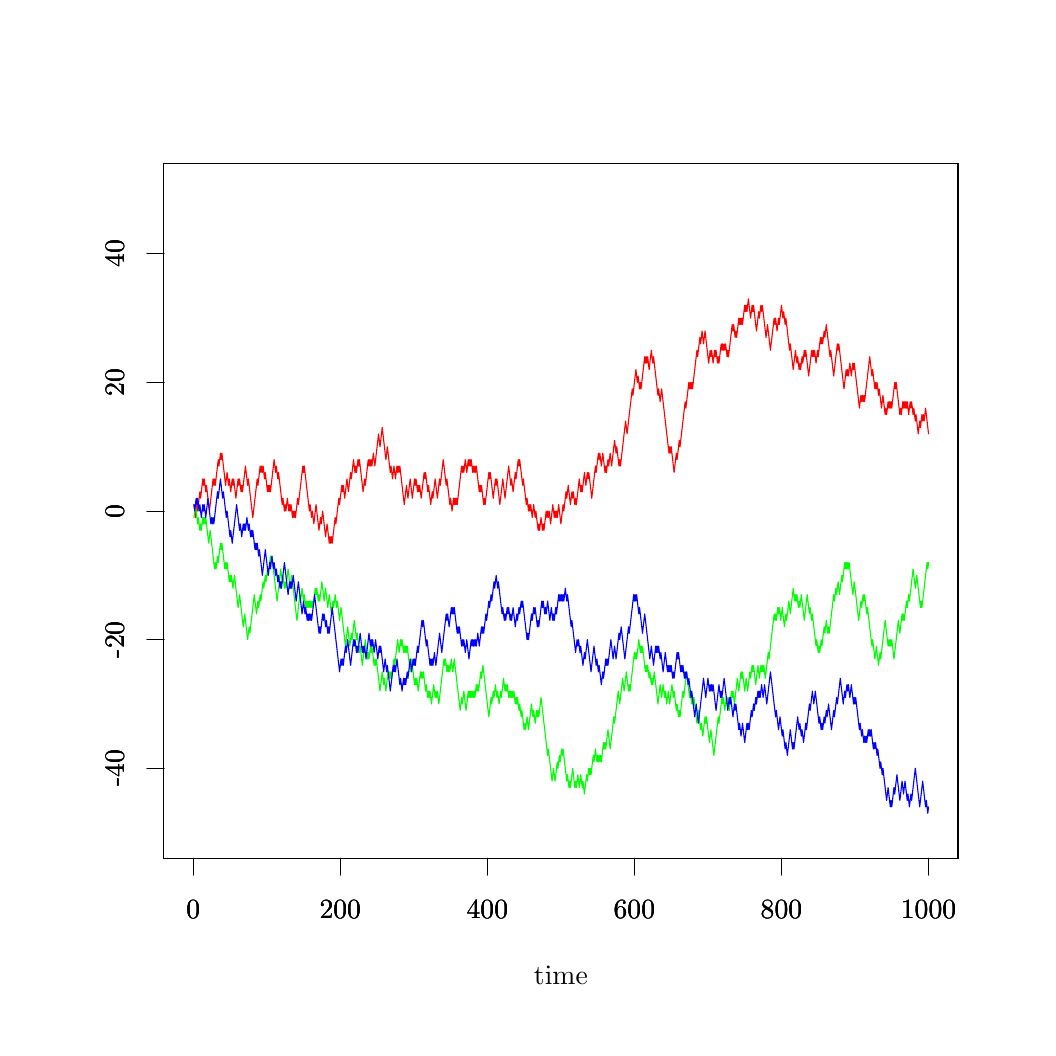
\begin{tikzpicture}[x=1pt,y=1pt] \definecolor{fillColor}{RGB}{255,255,255} \path[use as bounding box,fill=fillColor,fill opacity=0.00] (0,0) rectangle (361.35,361.35); \begin{scope} \path[clip] ( 49.20, 61.20) rectangle (336.15,312.15); \definecolor{drawColor}{RGB}{255,0,0}
\path[draw=drawColor,line width= 0.4pt,line join=round,line cap=round] ( 60.09,189.00) -- 	( 60.36,186.67) -- 	( 60.62,184.35) -- 	( 60.89,186.67) -- 	( 61.16,189.00) -- 	( 61.42,186.67) -- 	( 61.69,189.00) -- 	( 61.95,191.32) -- 	( 62.22,193.65) -- 	( 62.48,191.32) -- 	( 62.75,193.65) -- 	( 63.02,195.97) -- 	( 63.28,198.29) -- 	( 63.55,195.97) -- 	( 63.81,198.29) -- 	( 64.08,195.97) -- 	( 64.34,193.65) -- 	( 64.61,195.97) -- 	( 64.88,193.65) -- 	( 65.14,191.32) -- 	( 65.41,189.00) -- 	( 65.67,186.67) -- 	( 65.94,189.00) -- 	( 66.20,191.32) -- 	( 66.47,193.65) -- 	( 66.74,195.97) -- 	( 67.00,198.29) -- 	( 67.27,195.97) -- 	( 67.53,198.29) -- 	( 67.80,195.97) -- 	( 68.06,198.29) -- 	( 68.33,200.62) -- 	( 68.60,202.94) -- 	( 68.86,205.26) -- 	( 69.13,202.94) -- 	( 69.39,205.26) -- 	( 69.66,207.59) -- 	( 69.92,205.26) -- 	( 70.19,207.59) -- 	( 70.46,205.26) -- 	( 70.72,202.94) -- 	( 70.99,200.62) -- 	( 71.25,198.29) -- 	( 71.52,195.97) -- 	( 71.78,198.29) -- 	( 72.05,200.62) -- 	( 72.32,198.29) -- 	( 72.58,195.97) -- 	( 72.85,198.29) -- 	( 73.11,195.97) -- 	( 73.38,193.65) -- 	( 73.64,195.97) -- 	( 73.91,198.29) -- 	( 74.18,195.97) -- 	( 74.44,198.29) -- 	( 74.71,195.97) -- 	( 74.97,193.65) -- 	( 75.24,191.32) -- 	( 75.50,193.65) -- 	( 75.77,195.97) -- 	( 76.04,198.29) -- 	( 76.30,195.97) -- 	( 76.57,198.29) -- 	( 76.83,195.97) -- 	( 77.10,193.65) -- 	( 77.36,195.97) -- 	( 77.63,193.65) -- 	( 77.89,195.97) -- 	( 78.16,198.29) -- 	( 78.43,200.62) -- 	( 78.69,202.94) -- 	( 78.96,200.62) -- 	( 79.22,198.29) -- 	( 79.49,195.97) -- 	( 79.75,198.29) -- 	( 80.02,195.97) -- 	( 80.29,193.65) -- 	( 80.55,191.32) -- 	( 80.82,189.00) -- 	( 81.08,186.67) -- 	( 81.35,184.35) -- 	( 81.61,186.67) -- 	( 81.88,189.00) -- 	( 82.15,191.32) -- 	( 82.41,193.65) -- 	( 82.68,195.97) -- 	( 82.94,198.29) -- 	( 83.21,195.97) -- 	( 83.47,198.29) -- 	( 83.74,200.62) -- 	( 84.01,202.94) -- 	( 84.27,200.62) -- 	( 84.54,202.94) -- 	( 84.80,200.62) -- 	( 85.07,202.94) -- 	( 85.33,200.62) -- 	( 85.60,198.29) -- 	( 85.87,200.62) -- 	( 86.13,198.29) -- 	( 86.40,195.97) -- 	( 86.66,193.65) -- 	( 86.93,195.97) -- 	( 87.19,193.65) -- 	( 87.46,195.97) -- 	( 87.73,193.65) -- 	( 87.99,195.97) -- 	( 88.26,198.29) -- 	( 88.52,200.62) -- 	( 88.79,202.94) -- 	( 89.05,205.26) -- 	( 89.32,202.94) -- 	( 89.59,200.62) -- 	( 89.85,202.94) -- 	( 90.12,200.62) -- 	( 90.38,198.29) -- 	( 90.65,200.62) -- 	( 90.91,198.29) -- 	( 91.18,195.97) -- 	( 91.45,193.65) -- 	( 91.71,191.32) -- 	( 91.98,189.00) -- 	( 92.24,191.32) -- 	( 92.51,189.00) -- 	( 92.77,186.67) -- 	( 93.04,189.00) -- 	( 93.31,186.67) -- 	( 93.57,189.00) -- 	( 93.84,191.32) -- 	( 94.10,189.00) -- 	( 94.37,186.67) -- 	( 94.63,189.00) -- 	( 94.90,186.67) -- 	( 95.17,189.00) -- 	( 95.43,186.67) -- 	( 95.70,184.35) -- 	( 95.96,186.67) -- 	( 96.23,184.35) -- 	( 96.49,186.67) -- 	( 96.76,184.35) -- 	( 97.02,186.67) -- 	( 97.29,189.00) -- 	( 97.56,191.32) -- 	( 97.82,189.00) -- 	( 98.09,191.32) -- 	( 98.35,193.65) -- 	( 98.62,195.97) -- 	( 98.88,198.29) -- 	( 99.15,200.62) -- 	( 99.42,202.94) -- 	( 99.68,200.62) -- 	( 99.95,202.94) -- 	(100.21,200.62) -- 	(100.48,198.29) -- 	(100.74,195.97) -- 	(101.01,193.65) -- 	(101.28,191.32) -- 	(101.54,189.00) -- 	(101.81,186.67) -- 	(102.07,189.00) -- 	(102.34,186.67) -- 	(102.60,184.35) -- 	(102.87,186.67) -- 	(103.14,184.35) -- 	(103.40,182.03) -- 	(103.67,184.35) -- 	(103.93,186.67) -- 	(104.20,189.00) -- 	(104.46,186.67) -- 	(104.73,184.35) -- 	(105.00,182.03) -- 	(105.26,179.70) -- 	(105.53,182.03) -- 	(105.79,184.35) -- 	(106.06,182.03) -- 	(106.32,184.35) -- 	(106.59,186.67) -- 	(106.86,184.35) -- 	(107.12,182.03) -- 	(107.39,179.70) -- 	(107.65,177.38) -- 	(107.92,179.70) -- 	(108.18,182.03) -- 	(108.45,179.70) -- 	(108.72,177.38) -- 	(108.98,175.06) -- 	(109.25,177.38) -- 	(109.51,175.06) -- 	(109.78,177.38) -- 	(110.04,175.06) -- 	(110.31,177.38) -- 	(110.58,179.70) -- 	(110.84,182.03) -- 	(111.11,184.35) -- 	(111.37,182.03) -- 	(111.64,184.35) -- 	(111.90,186.67) -- 	(112.17,189.00) -- 	(112.44,191.32) -- 	(112.70,189.00) -- 	(112.97,191.32) -- 	(113.23,193.65) -- 	(113.50,195.97) -- 	(113.76,193.65) -- 	(114.03,195.97) -- 	(114.30,193.65) -- 	(114.56,191.32) -- 	(114.83,193.65) -- 	(115.09,195.97) -- 	(115.36,198.29) -- 	(115.62,195.97) -- 	(115.89,193.65) -- 	(116.15,195.97) -- 	(116.42,198.29) -- 	(116.69,200.62) -- 	(116.95,198.29) -- 	(117.22,200.62) -- 	(117.48,202.94) -- 	(117.75,205.26) -- 	(118.01,202.94) -- 	(118.28,200.62) -- 	(118.55,202.94) -- 	(118.81,200.62) -- 	(119.08,202.94) -- 	(119.34,205.26) -- 	(119.61,202.94) -- 	(119.87,205.26) -- 	(120.14,202.94) -- 	(120.41,200.62) -- 	(120.67,198.29) -- 	(120.94,195.97) -- 	(121.20,193.65) -- 	(121.47,195.97) -- 	(121.73,198.29) -- 	(122.00,195.97) -- 	(122.27,198.29) -- 	(122.53,200.62) -- 	(122.80,202.94) -- 	(123.06,205.26) -- 	(123.33,202.94) -- 	(123.59,205.26) -- 	(123.86,202.94) -- 	(124.13,205.26) -- 	(124.39,202.94) -- 	(124.66,205.26) -- 	(124.92,207.59) -- 	(125.19,205.26) -- 	(125.45,202.94) -- 	(125.72,205.26) -- 	(125.99,207.59) -- 	(126.25,209.91) -- 	(126.52,212.23) -- 	(126.78,214.56) -- 	(127.05,212.23) -- 	(127.31,209.91) -- 	(127.58,212.23) -- 	(127.85,214.56) -- 	(128.11,216.88) -- 	(128.38,214.56) -- 	(128.64,212.23) -- 	(128.91,209.91) -- 	(129.17,207.59) -- 	(129.44,205.26) -- 	(129.71,207.59) -- 	(129.97,209.91) -- 	(130.24,207.59) -- 	(130.50,205.26) -- 	(130.77,202.94) -- 	(131.03,200.62) -- 	(131.30,202.94) -- 	(131.57,200.62) -- 	(131.83,198.29) -- 	(132.10,200.62) -- 	(132.36,202.94) -- 	(132.63,200.62) -- 	(132.89,198.29) -- 	(133.16,200.62) -- 	(133.43,202.94) -- 	(133.69,200.62) -- 	(133.96,202.94) -- 	(134.22,200.62) -- 	(134.49,202.94) -- 	(134.75,200.62) -- 	(135.02,198.29) -- 	(135.28,195.97) -- 	(135.55,193.65) -- 	(135.82,191.32) -- 	(136.08,189.00) -- 	(136.35,191.32) -- 	(136.61,193.65) -- 	(136.88,195.97) -- 	(137.14,193.65) -- 	(137.41,191.32) -- 	(137.68,193.65) -- 	(137.94,195.97) -- 	(138.21,198.29) -- 	(138.47,195.97) -- 	(138.74,193.65) -- 	(139.00,191.32) -- 	(139.27,193.65) -- 	(139.54,195.97) -- 	(139.80,198.29) -- 	(140.07,195.97) -- 	(140.33,198.29) -- 	(140.60,195.97) -- 	(140.86,193.65) -- 	(141.13,195.97) -- 	(141.40,193.65) -- 	(141.66,195.97) -- 	(141.93,193.65) -- 	(142.19,191.32) -- 	(142.46,193.65) -- 	(142.72,195.97) -- 	(142.99,198.29) -- 	(143.26,200.62) -- 	(143.52,198.29) -- 	(143.79,200.62) -- 	(144.05,198.29) -- 	(144.32,195.97) -- 	(144.58,193.65) -- 	(144.85,195.97) -- 	(145.12,193.65) -- 	(145.38,191.32) -- 	(145.65,189.00) -- 	(145.91,191.32) -- 	(146.18,193.65) -- 	(146.44,191.32) -- 	(146.71,193.65) -- 	(146.98,195.97) -- 	(147.24,198.29) -- 	(147.51,195.97) -- 	(147.77,193.65) -- 	(148.04,191.32) -- 	(148.30,193.65) -- 	(148.57,195.97) -- 	(148.84,198.29) -- 	(149.10,195.97) -- 	(149.37,198.29) -- 	(149.63,200.62) -- 	(149.90,202.94) -- 	(150.16,205.26) -- 	(150.43,202.94) -- 	(150.70,200.62) -- 	(150.96,198.29) -- 	(151.23,195.97) -- 	(151.49,198.29) -- 	(151.76,195.97) -- 	(152.02,193.65) -- 	(152.29,191.32) -- 	(152.56,189.00) -- 	(152.82,191.32) -- 	(153.09,189.00) -- 	(153.35,186.67) -- 	(153.62,189.00) -- 	(153.88,191.32) -- 	(154.15,189.00) -- 	(154.41,191.32) -- 	(154.68,189.00) -- 	(154.95,191.32) -- 	(155.21,189.00) -- 	(155.48,191.32) -- 	(155.74,193.65) -- 	(156.01,195.97) -- 	(156.27,198.29) -- 	(156.54,200.62) -- 	(156.81,202.94) -- 	(157.07,200.62) -- 	(157.34,202.94) -- 	(157.60,200.62) -- 	(157.87,202.94) -- 	(158.13,205.26) -- 	(158.40,202.94) -- 	(158.67,200.62) -- 	(158.93,202.94) -- 	(159.20,205.26) -- 	(159.46,202.94) -- 	(159.73,205.26) -- 	(159.99,202.94) -- 	(160.26,205.26) -- 	(160.53,202.94) -- 	(160.79,200.62) -- 	(161.06,202.94) -- 	(161.32,200.62) -- 	(161.59,202.94) -- 	(161.85,200.62) -- 	(162.12,202.94) -- 	(162.39,200.62) -- 	(162.65,198.29) -- 	(162.92,195.97) -- 	(163.18,193.65) -- 	(163.45,195.97) -- 	(163.71,193.65) -- 	(163.98,195.97) -- 	(164.25,193.65) -- 	(164.51,191.32) -- 	(164.78,189.00) -- 	(165.04,191.32) -- 	(165.31,189.00) -- 	(165.57,191.32) -- 	(165.84,193.65) -- 	(166.11,195.97) -- 	(166.37,198.29) -- 	(166.64,200.62) -- 	(166.90,198.29) -- 	(167.17,200.62) -- 	(167.43,198.29) -- 	(167.70,195.97) -- 	(167.97,193.65) -- 	(168.23,191.32) -- 	(168.50,193.65) -- 	(168.76,195.97) -- 	(169.03,198.29) -- 	(169.29,195.97) -- 	(169.56,198.29) -- 	(169.83,195.97) -- 	(170.09,193.65) -- 	(170.36,191.32) -- 	(170.62,189.00) -- 	(170.89,191.32) -- 	(171.15,193.65) -- 	(171.42,195.97) -- 	(171.69,198.29) -- 	(171.95,195.97) -- 	(172.22,193.65) -- 	(172.48,191.32) -- 	(172.75,193.65) -- 	(173.01,195.97) -- 	(173.28,198.29) -- 	(173.54,200.62) -- 	(173.81,202.94) -- 	(174.08,200.62) -- 	(174.34,198.29) -- 	(174.61,195.97) -- 	(174.87,198.29) -- 	(175.14,195.97) -- 	(175.40,193.65) -- 	(175.67,195.97) -- 	(175.94,198.29) -- 	(176.20,200.62) -- 	(176.47,198.29) -- 	(176.73,200.62) -- 	(177.00,202.94) -- 	(177.26,205.26) -- 	(177.53,202.94) -- 	(177.80,205.26) -- 	(178.06,202.94) -- 	(178.33,200.62) -- 	(178.59,198.29) -- 	(178.86,195.97) -- 	(179.12,198.29) -- 	(179.39,195.97) -- 	(179.66,193.65) -- 	(179.92,191.32) -- 	(180.19,189.00) -- 	(180.45,191.32) -- 	(180.72,189.00) -- 	(180.98,186.67) -- 	(181.25,189.00) -- 	(181.52,186.67) -- 	(181.78,189.00) -- 	(182.05,186.67) -- 	(182.31,184.35) -- 	(182.58,186.67) -- 	(182.84,189.00) -- 	(183.11,186.67) -- 	(183.38,184.35) -- 	(183.64,186.67) -- 	(183.91,184.35) -- 	(184.17,182.03) -- 	(184.44,179.70) -- 	(184.70,182.03) -- 	(184.97,179.70) -- 	(185.24,182.03) -- 	(185.50,184.35) -- 	(185.77,182.03) -- 	(186.03,179.70) -- 	(186.30,182.03) -- 	(186.56,179.70) -- 	(186.83,182.03) -- 	(187.10,184.35) -- 	(187.36,186.67) -- 	(187.63,184.35) -- 	(187.89,186.67) -- 	(188.16,184.35) -- 	(188.42,186.67) -- 	(188.69,184.35) -- 	(188.96,182.03) -- 	(189.22,184.35) -- 	(189.49,186.67) -- 	(189.75,189.00) -- 	(190.02,186.67) -- 	(190.28,184.35) -- 	(190.55,186.67) -- 	(190.82,184.35) -- 	(191.08,186.67) -- 	(191.35,184.35) -- 	(191.61,186.67) -- 	(191.88,189.00) -- 	(192.14,186.67) -- 	(192.41,184.35) -- 	(192.68,182.03) -- 	(192.94,184.35) -- 	(193.21,186.67) -- 	(193.47,189.00) -- 	(193.74,186.67) -- 	(194.00,189.00) -- 	(194.27,191.32) -- 	(194.53,193.65) -- 	(194.80,191.32) -- 	(195.07,193.65) -- 	(195.33,195.97) -- 	(195.60,193.65) -- 	(195.86,191.32) -- 	(196.13,189.00) -- 	(196.39,191.32) -- 	(196.66,193.65) -- 	(196.93,191.32) -- 	(197.19,193.65) -- 	(197.46,191.32) -- 	(197.72,189.00) -- 	(197.99,191.32) -- 	(198.25,189.00) -- 	(198.52,191.32) -- 	(198.79,193.65) -- 	(199.05,195.97) -- 	(199.32,198.29) -- 	(199.58,195.97) -- 	(199.85,193.65) -- 	(200.11,195.97) -- 	(200.38,193.65) -- 	(200.65,195.97) -- 	(200.91,198.29) -- 	(201.18,200.62) -- 	(201.44,198.29) -- 	(201.71,195.97) -- 	(201.97,198.29) -- 	(202.24,200.62) -- 	(202.51,198.29) -- 	(202.77,200.62) -- 	(203.04,198.29) -- 	(203.30,195.97) -- 	(203.57,193.65) -- 	(203.83,191.32) -- 	(204.10,193.65) -- 	(204.37,195.97) -- 	(204.63,198.29) -- 	(204.90,200.62) -- 	(205.16,202.94) -- 	(205.43,200.62) -- 	(205.69,202.94) -- 	(205.96,205.26) -- 	(206.23,207.59) -- 	(206.49,205.26) -- 	(206.76,207.59) -- 	(207.02,205.26) -- 	(207.29,202.94) -- 	(207.55,205.26) -- 	(207.82,207.59) -- 	(208.09,205.26) -- 	(208.35,202.94) -- 	(208.62,200.62) -- 	(208.88,202.94) -- 	(209.15,200.62) -- 	(209.41,202.94) -- 	(209.68,205.26) -- 	(209.95,202.94) -- 	(210.21,205.26) -- 	(210.48,207.59) -- 	(210.74,205.26) -- 	(211.01,202.94) -- 	(211.27,205.26) -- 	(211.54,207.59) -- 	(211.80,209.91) -- 	(212.07,212.23) -- 	(212.34,209.91) -- 	(212.60,207.59) -- 	(212.87,209.91) -- 	(213.13,207.59) -- 	(213.40,205.26) -- 	(213.66,202.94) -- 	(213.93,205.26) -- 	(214.20,202.94) -- 	(214.46,205.26) -- 	(214.73,207.59) -- 	(214.99,209.91) -- 	(215.26,212.23) -- 	(215.52,214.56) -- 	(215.79,216.88) -- 	(216.06,219.21) -- 	(216.32,216.88) -- 	(216.59,214.56) -- 	(216.85,216.88) -- 	(217.12,219.21) -- 	(217.38,221.53) -- 	(217.65,223.85) -- 	(217.92,226.18) -- 	(218.18,228.50) -- 	(218.45,230.82) -- 	(218.71,228.50) -- 	(218.98,230.82) -- 	(219.24,233.15) -- 	(219.51,235.47) -- 	(219.78,237.79) -- 	(220.04,235.47) -- 	(220.31,233.15) -- 	(220.57,235.47) -- 	(220.84,233.15) -- 	(221.10,230.82) -- 	(221.37,233.15) -- 	(221.64,230.82) -- 	(221.90,233.15) -- 	(222.17,235.47) -- 	(222.43,237.79) -- 	(222.70,240.12) -- 	(222.96,242.44) -- 	(223.23,240.12) -- 	(223.50,242.44) -- 	(223.76,240.12) -- 	(224.03,242.44) -- 	(224.29,240.12) -- 	(224.56,237.79) -- 	(224.82,240.12) -- 	(225.09,242.44) -- 	(225.36,244.77) -- 	(225.62,242.44) -- 	(225.89,240.12) -- 	(226.15,242.44) -- 	(226.42,240.12) -- 	(226.68,237.79) -- 	(226.95,235.47) -- 	(227.22,233.15) -- 	(227.48,230.82) -- 	(227.75,228.50) -- 	(228.01,230.82) -- 	(228.28,228.50) -- 	(228.54,226.18) -- 	(228.81,228.50) -- 	(229.08,230.82) -- 	(229.34,228.50) -- 	(229.61,226.18) -- 	(229.87,223.85) -- 	(230.14,221.53) -- 	(230.40,219.21) -- 	(230.67,216.88) -- 	(230.93,214.56) -- 	(231.20,212.23) -- 	(231.47,209.91) -- 	(231.73,207.59) -- 	(232.00,209.91) -- 	(232.26,207.59) -- 	(232.53,209.91) -- 	(232.79,207.59) -- 	(233.06,205.26) -- 	(233.33,202.94) -- 	(233.59,200.62) -- 	(233.86,202.94) -- 	(234.12,205.26) -- 	(234.39,207.59) -- 	(234.65,205.26) -- 	(234.92,207.59) -- 	(235.19,209.91) -- 	(235.45,212.23) -- 	(235.72,209.91) -- 	(235.98,212.23) -- 	(236.25,214.56) -- 	(236.51,216.88) -- 	(236.78,219.21) -- 	(237.05,221.53) -- 	(237.31,223.85) -- 	(237.58,226.18) -- 	(237.84,223.85) -- 	(238.11,226.18) -- 	(238.37,228.50) -- 	(238.64,230.82) -- 	(238.91,233.15) -- 	(239.17,230.82) -- 	(239.44,233.15) -- 	(239.70,230.82) -- 	(239.97,233.15) -- 	(240.23,230.82) -- 	(240.50,233.15) -- 	(240.77,235.47) -- 	(241.03,237.79) -- 	(241.30,240.12) -- 	(241.56,242.44) -- 	(241.83,244.77) -- 	(242.09,242.44) -- 	(242.36,244.77) -- 	(242.63,247.09) -- 	(242.89,249.41) -- 	(243.16,247.09) -- 	(243.42,249.41) -- 	(243.69,251.74) -- 	(243.95,249.41) -- 	(244.22,247.09) -- 	(244.49,249.41) -- 	(244.75,251.74) -- 	(245.02,249.41) -- 	(245.28,247.09) -- 	(245.55,244.77) -- 	(245.81,242.44) -- 	(246.08,240.12) -- 	(246.35,242.44) -- 	(246.61,244.77) -- 	(246.88,242.44) -- 	(247.14,244.77) -- 	(247.41,242.44) -- 	(247.67,240.12) -- 	(247.94,242.44) -- 	(248.21,244.77) -- 	(248.47,242.44) -- 	(248.74,244.77) -- 	(249.00,242.44) -- 	(249.27,240.12) -- 	(249.53,242.44) -- 	(249.80,240.12) -- 	(250.06,242.44) -- 	(250.33,244.77) -- 	(250.60,247.09) -- 	(250.86,244.77) -- 	(251.13,247.09) -- 	(251.39,244.77) -- 	(251.66,247.09) -- 	(251.92,244.77) -- 	(252.19,247.09) -- 	(252.46,244.77) -- 	(252.72,242.44) -- 	(252.99,244.77) -- 	(253.25,242.44) -- 	(253.52,244.77) -- 	(253.78,247.09) -- 	(254.05,249.41) -- 	(254.32,251.74) -- 	(254.58,254.06) -- 	(254.85,251.74) -- 	(255.11,254.06) -- 	(255.38,251.74) -- 	(255.64,249.41) -- 	(255.91,251.74) -- 	(256.18,249.41) -- 	(256.44,251.74) -- 	(256.71,254.06) -- 	(256.97,256.38) -- 	(257.24,254.06) -- 	(257.50,256.38) -- 	(257.77,254.06) -- 	(258.04,256.38) -- 	(258.30,254.06) -- 	(258.57,256.38) -- 	(258.83,258.71) -- 	(259.10,261.03) -- 	(259.36,258.71) -- 	(259.63,261.03) -- 	(259.90,258.71) -- 	(260.16,261.03) -- 	(260.43,263.35) -- 	(260.69,261.03) -- 	(260.96,258.71) -- 	(261.22,256.38) -- 	(261.49,258.71) -- 	(261.76,261.03) -- 	(262.02,258.71) -- 	(262.29,261.03) -- 	(262.55,258.71) -- 	(262.82,256.38) -- 	(263.08,254.06) -- 	(263.35,251.74) -- 	(263.62,254.06) -- 	(263.88,256.38) -- 	(264.15,258.71) -- 	(264.41,256.38) -- 	(264.68,258.71) -- 	(264.94,261.03) -- 	(265.21,258.71) -- 	(265.48,261.03) -- 	(265.74,258.71) -- 	(266.01,256.38) -- 	(266.27,254.06) -- 	(266.54,251.74) -- 	(266.80,249.41) -- 	(267.07,251.74) -- 	(267.34,254.06) -- 	(267.60,251.74) -- 	(267.87,249.41) -- 	(268.13,247.09) -- 	(268.40,244.77) -- 	(268.66,247.09) -- 	(268.93,249.41) -- 	(269.19,251.74) -- 	(269.46,254.06) -- 	(269.73,256.38) -- 	(269.99,254.06) -- 	(270.26,256.38) -- 	(270.52,254.06) -- 	(270.79,251.74) -- 	(271.05,254.06) -- 	(271.32,256.38) -- 	(271.59,254.06) -- 	(271.85,256.38) -- 	(272.12,258.71) -- 	(272.38,261.03) -- 	(272.65,258.71) -- 	(272.91,256.38) -- 	(273.18,258.71) -- 	(273.45,256.38) -- 	(273.71,254.06) -- 	(273.98,256.38) -- 	(274.24,254.06) -- 	(274.51,251.74) -- 	(274.77,249.41) -- 	(275.04,247.09) -- 	(275.31,244.77) -- 	(275.57,247.09) -- 	(275.84,244.77) -- 	(276.10,242.44) -- 	(276.37,240.12) -- 	(276.63,237.79) -- 	(276.90,240.12) -- 	(277.17,242.44) -- 	(277.43,244.77) -- 	(277.70,242.44) -- 	(277.96,240.12) -- 	(278.23,242.44) -- 	(278.49,240.12) -- 	(278.76,237.79) -- 	(279.03,240.12) -- 	(279.29,237.79) -- 	(279.56,240.12) -- 	(279.82,242.44) -- 	(280.09,240.12) -- 	(280.35,242.44) -- 	(280.62,244.77) -- 	(280.89,242.44) -- 	(281.15,244.77) -- 	(281.42,242.44) -- 	(281.68,240.12) -- 	(281.95,237.79) -- 	(282.21,235.47) -- 	(282.48,237.79) -- 	(282.75,240.12) -- 	(283.01,242.44) -- 	(283.28,244.77) -- 	(283.54,242.44) -- 	(283.81,244.77) -- 	(284.07,242.44) -- 	(284.34,244.77) -- 	(284.61,242.44) -- 	(284.87,240.12) -- 	(285.14,242.44) -- 	(285.40,244.77) -- 	(285.67,242.44) -- 	(285.93,244.77) -- 	(286.20,247.09) -- 	(286.47,249.41) -- 	(286.73,247.09) -- 	(287.00,249.41) -- 	(287.26,247.09) -- 	(287.53,249.41) -- 	(287.79,251.74) -- 	(288.06,249.41) -- 	(288.32,251.74) -- 	(288.59,254.06) -- 	(288.86,251.74) -- 	(289.12,249.41) -- 	(289.39,247.09) -- 	(289.65,244.77) -- 	(289.92,242.44) -- 	(290.18,244.77) -- 	(290.45,242.44) -- 	(290.72,240.12) -- 	(290.98,237.79) -- 	(291.25,235.47) -- 	(291.51,237.79) -- 	(291.78,240.12) -- 	(292.04,242.44) -- 	(292.31,244.77) -- 	(292.58,247.09) -- 	(292.84,244.77) -- 	(293.11,247.09) -- 	(293.37,244.77) -- 	(293.64,242.44) -- 	(293.90,240.12) -- 	(294.17,237.79) -- 	(294.44,235.47) -- 	(294.70,233.15) -- 	(294.97,230.82) -- 	(295.23,233.15) -- 	(295.50,235.47) -- 	(295.76,237.79) -- 	(296.03,235.47) -- 	(296.30,237.79) -- 	(296.56,235.47) -- 	(296.83,237.79) -- 	(297.09,240.12) -- 	(297.36,237.79) -- 	(297.62,235.47) -- 	(297.89,237.79) -- 	(298.16,240.12) -- 	(298.42,237.79) -- 	(298.69,240.12) -- 	(298.95,237.79) -- 	(299.22,235.47) -- 	(299.48,233.15) -- 	(299.75,230.82) -- 	(300.02,228.50) -- 	(300.28,226.18) -- 	(300.55,223.85) -- 	(300.81,226.18) -- 	(301.08,228.50) -- 	(301.34,226.18) -- 	(301.61,228.50) -- 	(301.88,226.18) -- 	(302.14,228.50) -- 	(302.41,226.18) -- 	(302.67,228.50) -- 	(302.94,230.82) -- 	(303.20,233.15) -- 	(303.47,235.47) -- 	(303.74,237.79) -- 	(304.00,240.12) -- 	(304.27,242.44) -- 	(304.53,240.12) -- 	(304.80,237.79) -- 	(305.06,235.47) -- 	(305.33,237.79) -- 	(305.60,235.47) -- 	(305.86,233.15) -- 	(306.13,230.82) -- 	(306.39,233.15) -- 	(306.66,230.82) -- 	(306.92,233.15) -- 	(307.19,230.82) -- 	(307.45,228.50) -- 	(307.72,230.82) -- 	(307.99,228.50) -- 	(308.25,226.18) -- 	(308.52,223.85) -- 	(308.78,226.18) -- 	(309.05,228.50) -- 	(309.31,226.18) -- 	(309.58,223.85) -- 	(309.85,221.53) -- 	(310.11,223.85) -- 	(310.38,221.53) -- 	(310.64,223.85) -- 	(310.91,226.18) -- 	(311.17,223.85) -- 	(311.44,226.18) -- 	(311.71,223.85) -- 	(311.97,226.18) -- 	(312.24,223.85) -- 	(312.50,226.18) -- 	(312.77,228.50) -- 	(313.03,230.82) -- 	(313.30,233.15) -- 	(313.57,230.82) -- 	(313.83,233.15) -- 	(314.10,230.82) -- 	(314.36,228.50) -- 	(314.63,226.18) -- 	(314.89,223.85) -- 	(315.16,221.53) -- 	(315.43,223.85) -- 	(315.69,221.53) -- 	(315.96,223.85) -- 	(316.22,226.18) -- 	(316.49,223.85) -- 	(316.75,226.18) -- 	(317.02,223.85) -- 	(317.29,226.18) -- 	(317.55,223.85) -- 	(317.82,226.18) -- 	(318.08,223.85) -- 	(318.35,221.53) -- 	(318.61,223.85) -- 	(318.88,226.18) -- 	(319.15,223.85) -- 	(319.41,226.18) -- 	(319.68,223.85) -- 	(319.94,221.53) -- 	(320.21,223.85) -- 	(320.47,221.53) -- 	(320.74,219.21) -- 	(321.01,221.53) -- 	(321.27,219.21) -- 	(321.54,216.88) -- 	(321.80,214.56) -- 	(322.07,216.88) -- 	(322.33,219.21) -- 	(322.60,216.88) -- 	(322.87,219.21) -- 	(323.13,221.53) -- 	(323.40,219.21) -- 	(323.66,221.53) -- 	(323.93,219.21) -- 	(324.19,221.53) -- 	(324.46,223.85) -- 	(324.73,221.53) -- 	(324.99,219.21) -- 	(325.26,216.88) -- 	(325.52,214.56); \end{scope} \begin{scope} \path[clip] (  0.00,  0.00) rectangle (361.35,361.35); \definecolor{drawColor}{RGB}{0,0,0}
\path[draw=drawColor,line width= 0.4pt,line join=round,line cap=round] ( 59.83, 61.20) -- (325.52, 61.20);
\path[draw=drawColor,line width= 0.4pt,line join=round,line cap=round] ( 59.83, 61.20) -- ( 59.83, 55.20);
\path[draw=drawColor,line width= 0.4pt,line join=round,line cap=round] (112.97, 61.20) -- (112.97, 55.20);
\path[draw=drawColor,line width= 0.4pt,line join=round,line cap=round] (166.11, 61.20) -- (166.11, 55.20);
\path[draw=drawColor,line width= 0.4pt,line join=round,line cap=round] (219.24, 61.20) -- (219.24, 55.20);
\path[draw=drawColor,line width= 0.4pt,line join=round,line cap=round] (272.38, 61.20) -- (272.38, 55.20);
\path[draw=drawColor,line width= 0.4pt,line join=round,line cap=round] (325.52, 61.20) -- (325.52, 55.20);
\node[text=drawColor,anchor=base,inner sep=0pt, outer sep=0pt, scale=  1.00] at ( 59.83, 39.60) {0};
\node[text=drawColor,anchor=base,inner sep=0pt, outer sep=0pt, scale=  1.00] at (112.97, 39.60) {200};
\node[text=drawColor,anchor=base,inner sep=0pt, outer sep=0pt, scale=  1.00] at (166.11, 39.60) {400};
\node[text=drawColor,anchor=base,inner sep=0pt, outer sep=0pt, scale=  1.00] at (219.24, 39.60) {600};
\node[text=drawColor,anchor=base,inner sep=0pt, outer sep=0pt, scale=  1.00] at (272.38, 39.60) {800};
\node[text=drawColor,anchor=base,inner sep=0pt, outer sep=0pt, scale=  1.00] at (325.52, 39.60) {1000};
\path[draw=drawColor,line width= 0.4pt,line join=round,line cap=round] ( 49.20, 93.73) -- ( 49.20,279.62);
\path[draw=drawColor,line width= 0.4pt,line join=round,line cap=round] ( 49.20, 93.73) -- ( 43.20, 93.73);
\path[draw=drawColor,line width= 0.4pt,line join=round,line cap=round] ( 49.20,140.20) -- ( 43.20,140.20);
\path[draw=drawColor,line width= 0.4pt,line join=round,line cap=round] ( 49.20,186.67) -- ( 43.20,186.67);
\path[draw=drawColor,line width= 0.4pt,line join=round,line cap=round] ( 49.20,233.15) -- ( 43.20,233.15);
\path[draw=drawColor,line width= 0.4pt,line join=round,line cap=round] ( 49.20,279.62) -- ( 43.20,279.62);
\node[text=drawColor,rotate= 90.00,anchor=base,inner sep=0pt, outer sep=0pt, scale=  1.00] at ( 34.80, 93.73) {-40};
\node[text=drawColor,rotate= 90.00,anchor=base,inner sep=0pt, outer sep=0pt, scale=  1.00] at ( 34.80,140.20) {-20};
\node[text=drawColor,rotate= 90.00,anchor=base,inner sep=0pt, outer sep=0pt, scale=  1.00] at ( 34.80,186.67) {0};
\node[text=drawColor,rotate= 90.00,anchor=base,inner sep=0pt, outer sep=0pt, scale=  1.00] at ( 34.80,233.15) {20};
\node[text=drawColor,rotate= 90.00,anchor=base,inner sep=0pt, outer sep=0pt, scale=  1.00] at ( 34.80,279.62) {40};
\path[draw=drawColor,line width= 0.4pt,line join=round,line cap=round] ( 49.20, 61.20) -- 	(336.15, 61.20) -- 	(336.15,312.15) -- 	( 49.20,312.15) -- 	( 49.20, 61.20); \end{scope} \begin{scope} \path[clip] (  0.00,  0.00) rectangle (361.35,361.35); \definecolor{drawColor}{RGB}{0,0,0}
\node[text=drawColor,anchor=base,inner sep=0pt, outer sep=0pt, scale=  1.00] at (192.68, 15.60) {time}; \end{scope} \begin{scope} \path[clip] ( 49.20, 61.20) rectangle (336.15,312.15); \definecolor{drawColor}{RGB}{0,255,0}
\path[draw=drawColor,line width= 0.4pt,line join=round,line cap=round] ( 60.09,184.35) -- 	( 60.36,186.67) -- 	( 60.62,189.00) -- 	( 60.89,186.67) -- 	( 61.16,184.35) -- 	( 61.42,182.03) -- 	( 61.69,184.35) -- 	( 61.95,182.03) -- 	( 62.22,179.70) -- 	( 62.48,182.03) -- 	( 62.75,179.70) -- 	( 63.02,182.03) -- 	( 63.28,184.35) -- 	( 63.55,182.03) -- 	( 63.81,184.35) -- 	( 64.08,182.03) -- 	( 64.34,184.35) -- 	( 64.61,182.03) -- 	( 64.88,179.70) -- 	( 65.14,177.38) -- 	( 65.41,175.06) -- 	( 65.67,177.38) -- 	( 65.94,179.70) -- 	( 66.20,177.38) -- 	( 66.47,175.06) -- 	( 66.74,172.73) -- 	( 67.00,170.41) -- 	( 67.27,168.09) -- 	( 67.53,165.76) -- 	( 67.80,168.09) -- 	( 68.06,165.76) -- 	( 68.33,168.09) -- 	( 68.60,170.41) -- 	( 68.86,168.09) -- 	( 69.13,170.41) -- 	( 69.39,172.73) -- 	( 69.66,175.06) -- 	( 69.92,172.73) -- 	( 70.19,175.06) -- 	( 70.46,172.73) -- 	( 70.72,170.41) -- 	( 70.99,168.09) -- 	( 71.25,165.76) -- 	( 71.52,168.09) -- 	( 71.78,165.76) -- 	( 72.05,168.09) -- 	( 72.32,165.76) -- 	( 72.58,163.44) -- 	( 72.85,161.12) -- 	( 73.11,163.44) -- 	( 73.38,161.12) -- 	( 73.64,163.44) -- 	( 73.91,161.12) -- 	( 74.18,158.79) -- 	( 74.44,161.12) -- 	( 74.71,163.44) -- 	( 74.97,161.12) -- 	( 75.24,158.79) -- 	( 75.50,156.47) -- 	( 75.77,154.14) -- 	( 76.04,151.82) -- 	( 76.30,154.14) -- 	( 76.57,156.47) -- 	( 76.83,154.14) -- 	( 77.10,151.82) -- 	( 77.36,149.50) -- 	( 77.63,147.17) -- 	( 77.89,144.85) -- 	( 78.16,147.17) -- 	( 78.43,149.50) -- 	( 78.69,147.17) -- 	( 78.96,144.85) -- 	( 79.22,142.53) -- 	( 79.49,140.20) -- 	( 79.75,142.53) -- 	( 80.02,144.85) -- 	( 80.29,142.53) -- 	( 80.55,144.85) -- 	( 80.82,147.17) -- 	( 81.08,149.50) -- 	( 81.35,151.82) -- 	( 81.61,154.14) -- 	( 81.88,156.47) -- 	( 82.15,154.14) -- 	( 82.41,151.82) -- 	( 82.68,149.50) -- 	( 82.94,151.82) -- 	( 83.21,154.14) -- 	( 83.47,151.82) -- 	( 83.74,154.14) -- 	( 84.01,156.47) -- 	( 84.27,154.14) -- 	( 84.54,156.47) -- 	( 84.80,158.79) -- 	( 85.07,161.12) -- 	( 85.33,158.79) -- 	( 85.60,161.12) -- 	( 85.87,163.44) -- 	( 86.13,161.12) -- 	( 86.40,163.44) -- 	( 86.66,165.76) -- 	( 86.93,163.44) -- 	( 87.19,165.76) -- 	( 87.46,168.09) -- 	( 87.73,170.41) -- 	( 87.99,168.09) -- 	( 88.26,170.41) -- 	( 88.52,168.09) -- 	( 88.79,165.76) -- 	( 89.05,163.44) -- 	( 89.32,161.12) -- 	( 89.59,158.79) -- 	( 89.85,156.47) -- 	( 90.12,154.14) -- 	( 90.38,156.47) -- 	( 90.65,158.79) -- 	( 90.91,161.12) -- 	( 91.18,163.44) -- 	( 91.45,165.76) -- 	( 91.71,163.44) -- 	( 91.98,161.12) -- 	( 92.24,163.44) -- 	( 92.51,161.12) -- 	( 92.77,158.79) -- 	( 93.04,161.12) -- 	( 93.31,158.79) -- 	( 93.57,161.12) -- 	( 93.84,163.44) -- 	( 94.10,165.76) -- 	( 94.37,163.44) -- 	( 94.63,161.12) -- 	( 94.90,158.79) -- 	( 95.17,161.12) -- 	( 95.43,163.44) -- 	( 95.70,161.12) -- 	( 95.96,158.79) -- 	( 96.23,156.47) -- 	( 96.49,154.14) -- 	( 96.76,151.82) -- 	( 97.02,149.50) -- 	( 97.29,147.17) -- 	( 97.56,149.50) -- 	( 97.82,151.82) -- 	( 98.09,154.14) -- 	( 98.35,156.47) -- 	( 98.62,154.14) -- 	( 98.88,156.47) -- 	( 99.15,158.79) -- 	( 99.42,156.47) -- 	( 99.68,154.14) -- 	( 99.95,156.47) -- 	(100.21,154.14) -- 	(100.48,151.82) -- 	(100.74,154.14) -- 	(101.01,151.82) -- 	(101.28,154.14) -- 	(101.54,151.82) -- 	(101.81,154.14) -- 	(102.07,151.82) -- 	(102.34,154.14) -- 	(102.60,151.82) -- 	(102.87,154.14) -- 	(103.14,151.82) -- 	(103.40,154.14) -- 	(103.67,156.47) -- 	(103.93,158.79) -- 	(104.20,156.47) -- 	(104.46,158.79) -- 	(104.73,156.47) -- 	(105.00,154.14) -- 	(105.26,156.47) -- 	(105.53,154.14) -- 	(105.79,156.47) -- 	(106.06,158.79) -- 	(106.32,161.12) -- 	(106.59,158.79) -- 	(106.86,156.47) -- 	(107.12,154.14) -- 	(107.39,156.47) -- 	(107.65,158.79) -- 	(107.92,156.47) -- 	(108.18,154.14) -- 	(108.45,151.82) -- 	(108.72,154.14) -- 	(108.98,156.47) -- 	(109.25,154.14) -- 	(109.51,151.82) -- 	(109.78,149.50) -- 	(110.04,151.82) -- 	(110.31,154.14) -- 	(110.58,151.82) -- 	(110.84,154.14) -- 	(111.11,156.47) -- 	(111.37,154.14) -- 	(111.64,151.82) -- 	(111.90,154.14) -- 	(112.17,151.82) -- 	(112.44,149.50) -- 	(112.70,147.17) -- 	(112.97,149.50) -- 	(113.23,151.82) -- 	(113.50,149.50) -- 	(113.76,147.17) -- 	(114.03,144.85) -- 	(114.30,142.53) -- 	(114.56,140.20) -- 	(114.83,137.88) -- 	(115.09,140.20) -- 	(115.36,142.53) -- 	(115.62,144.85) -- 	(115.89,142.53) -- 	(116.15,140.20) -- 	(116.42,137.88) -- 	(116.69,140.20) -- 	(116.95,142.53) -- 	(117.22,140.20) -- 	(117.48,142.53) -- 	(117.75,144.85) -- 	(118.01,147.17) -- 	(118.28,144.85) -- 	(118.55,142.53) -- 	(118.81,140.20) -- 	(119.08,142.53) -- 	(119.34,140.20) -- 	(119.61,137.88) -- 	(119.87,135.56) -- 	(120.14,137.88) -- 	(120.41,135.56) -- 	(120.67,133.23) -- 	(120.94,130.91) -- 	(121.20,133.23) -- 	(121.47,135.56) -- 	(121.73,137.88) -- 	(122.00,140.20) -- 	(122.27,137.88) -- 	(122.53,135.56) -- 	(122.80,133.23) -- 	(123.06,135.56) -- 	(123.33,133.23) -- 	(123.59,135.56) -- 	(123.86,137.88) -- 	(124.13,135.56) -- 	(124.39,137.88) -- 	(124.66,135.56) -- 	(124.92,133.23) -- 	(125.19,130.91) -- 	(125.45,133.23) -- 	(125.72,130.91) -- 	(125.99,133.23) -- 	(126.25,130.91) -- 	(126.52,128.58) -- 	(126.78,126.26) -- 	(127.05,123.94) -- 	(127.31,121.61) -- 	(127.58,123.94) -- 	(127.85,126.26) -- 	(128.11,128.58) -- 	(128.38,126.26) -- 	(128.64,123.94) -- 	(128.91,126.26) -- 	(129.17,123.94) -- 	(129.44,121.61) -- 	(129.71,123.94) -- 	(129.97,126.26) -- 	(130.24,128.58) -- 	(130.50,126.26) -- 	(130.77,128.58) -- 	(131.03,126.26) -- 	(131.30,128.58) -- 	(131.57,126.26) -- 	(131.83,128.58) -- 	(132.10,130.91) -- 	(132.36,133.23) -- 	(132.63,130.91) -- 	(132.89,133.23) -- 	(133.16,135.56) -- 	(133.43,137.88) -- 	(133.69,140.20) -- 	(133.96,137.88) -- 	(134.22,135.56) -- 	(134.49,137.88) -- 	(134.75,140.20) -- 	(135.02,137.88) -- 	(135.28,140.20) -- 	(135.55,137.88) -- 	(135.82,135.56) -- 	(136.08,137.88) -- 	(136.35,135.56) -- 	(136.61,137.88) -- 	(136.88,135.56) -- 	(137.14,137.88) -- 	(137.41,135.56) -- 	(137.68,133.23) -- 	(137.94,130.91) -- 	(138.21,128.58) -- 	(138.47,130.91) -- 	(138.74,133.23) -- 	(139.00,130.91) -- 	(139.27,128.58) -- 	(139.54,126.26) -- 	(139.80,123.94) -- 	(140.07,126.26) -- 	(140.33,123.94) -- 	(140.60,126.26) -- 	(140.86,123.94) -- 	(141.13,121.61) -- 	(141.40,123.94) -- 	(141.66,126.26) -- 	(141.93,128.58) -- 	(142.19,126.26) -- 	(142.46,128.58) -- 	(142.72,126.26) -- 	(142.99,128.58) -- 	(143.26,126.26) -- 	(143.52,123.94) -- 	(143.79,121.61) -- 	(144.05,123.94) -- 	(144.32,121.61) -- 	(144.58,119.29) -- 	(144.85,121.61) -- 	(145.12,119.29) -- 	(145.38,121.61) -- 	(145.65,119.29) -- 	(145.91,116.97) -- 	(146.18,119.29) -- 	(146.44,121.61) -- 	(146.71,123.94) -- 	(146.98,121.61) -- 	(147.24,119.29) -- 	(147.51,121.61) -- 	(147.77,119.29) -- 	(148.04,121.61) -- 	(148.30,119.29) -- 	(148.57,116.97) -- 	(148.84,119.29) -- 	(149.10,121.61) -- 	(149.37,123.94) -- 	(149.63,126.26) -- 	(149.90,128.58) -- 	(150.16,130.91) -- 	(150.43,133.23) -- 	(150.70,130.91) -- 	(150.96,133.23) -- 	(151.23,130.91) -- 	(151.49,128.58) -- 	(151.76,130.91) -- 	(152.02,128.58) -- 	(152.29,130.91) -- 	(152.56,128.58) -- 	(152.82,130.91) -- 	(153.09,133.23) -- 	(153.35,130.91) -- 	(153.62,128.58) -- 	(153.88,130.91) -- 	(154.15,133.23) -- 	(154.41,130.91) -- 	(154.68,128.58) -- 	(154.95,126.26) -- 	(155.21,123.94) -- 	(155.48,121.61) -- 	(155.74,119.29) -- 	(156.01,116.97) -- 	(156.27,114.64) -- 	(156.54,116.97) -- 	(156.81,119.29) -- 	(157.07,116.97) -- 	(157.34,119.29) -- 	(157.60,121.61) -- 	(157.87,119.29) -- 	(158.13,116.97) -- 	(158.40,114.64) -- 	(158.67,116.97) -- 	(158.93,119.29) -- 	(159.20,121.61) -- 	(159.46,119.29) -- 	(159.73,121.61) -- 	(159.99,119.29) -- 	(160.26,121.61) -- 	(160.53,119.29) -- 	(160.79,121.61) -- 	(161.06,119.29) -- 	(161.32,121.61) -- 	(161.59,119.29) -- 	(161.85,121.61) -- 	(162.12,123.94) -- 	(162.39,121.61) -- 	(162.65,123.94) -- 	(162.92,121.61) -- 	(163.18,123.94) -- 	(163.45,126.26) -- 	(163.71,128.58) -- 	(163.98,126.26) -- 	(164.25,128.58) -- 	(164.51,130.91) -- 	(164.78,128.58) -- 	(165.04,126.26) -- 	(165.31,123.94) -- 	(165.57,121.61) -- 	(165.84,119.29) -- 	(166.11,116.97) -- 	(166.37,114.64) -- 	(166.64,112.32) -- 	(166.90,114.64) -- 	(167.17,116.97) -- 	(167.43,119.29) -- 	(167.70,116.97) -- 	(167.97,119.29) -- 	(168.23,121.61) -- 	(168.50,119.29) -- 	(168.76,121.61) -- 	(169.03,123.94) -- 	(169.29,121.61) -- 	(169.56,119.29) -- 	(169.83,121.61) -- 	(170.09,119.29) -- 	(170.36,116.97) -- 	(170.62,119.29) -- 	(170.89,121.61) -- 	(171.15,119.29) -- 	(171.42,121.61) -- 	(171.69,123.94) -- 	(171.95,126.26) -- 	(172.22,123.94) -- 	(172.48,121.61) -- 	(172.75,123.94) -- 	(173.01,121.61) -- 	(173.28,123.94) -- 	(173.54,121.61) -- 	(173.81,119.29) -- 	(174.08,121.61) -- 	(174.34,119.29) -- 	(174.61,121.61) -- 	(174.87,119.29) -- 	(175.14,121.61) -- 	(175.40,119.29) -- 	(175.67,121.61) -- 	(175.94,119.29) -- 	(176.20,116.97) -- 	(176.47,119.29) -- 	(176.73,116.97) -- 	(177.00,119.29) -- 	(177.26,116.97) -- 	(177.53,114.64) -- 	(177.80,116.97) -- 	(178.06,114.64) -- 	(178.33,112.32) -- 	(178.59,114.64) -- 	(178.86,112.32) -- 	(179.12,110.00) -- 	(179.39,107.67) -- 	(179.66,110.00) -- 	(179.92,107.67) -- 	(180.19,110.00) -- 	(180.45,112.32) -- 	(180.72,110.00) -- 	(180.98,107.67) -- 	(181.25,110.00) -- 	(181.52,112.32) -- 	(181.78,114.64) -- 	(182.05,116.97) -- 	(182.31,114.64) -- 	(182.58,112.32) -- 	(182.84,114.64) -- 	(183.11,112.32) -- 	(183.38,110.00) -- 	(183.64,112.32) -- 	(183.91,114.64) -- 	(184.17,112.32) -- 	(184.44,114.64) -- 	(184.70,112.32) -- 	(184.97,114.64) -- 	(185.24,116.97) -- 	(185.50,119.29) -- 	(185.77,116.97) -- 	(186.03,114.64) -- 	(186.30,112.32) -- 	(186.56,110.00) -- 	(186.83,107.67) -- 	(187.10,105.35) -- 	(187.36,103.02) -- 	(187.63,100.70) -- 	(187.89, 98.38) -- 	(188.16,100.70) -- 	(188.42, 98.38) -- 	(188.69, 96.05) -- 	(188.96, 93.73) -- 	(189.22, 91.41) -- 	(189.49, 89.08) -- 	(189.75, 91.41) -- 	(190.02, 93.73) -- 	(190.28, 91.41) -- 	(190.55, 89.08) -- 	(190.82, 91.41) -- 	(191.08, 93.73) -- 	(191.35, 96.05) -- 	(191.61, 93.73) -- 	(191.88, 96.05) -- 	(192.14, 98.38) -- 	(192.41, 96.05) -- 	(192.68, 98.38) -- 	(192.94,100.70) -- 	(193.21, 98.38) -- 	(193.47,100.70) -- 	(193.74, 98.38) -- 	(194.00, 96.05) -- 	(194.27, 93.73) -- 	(194.53, 91.41) -- 	(194.80, 89.08) -- 	(195.07, 91.41) -- 	(195.33, 89.08) -- 	(195.60, 86.76) -- 	(195.86, 89.08) -- 	(196.13, 86.76) -- 	(196.39, 89.08) -- 	(196.66, 91.41) -- 	(196.93, 93.73) -- 	(197.19, 91.41) -- 	(197.46, 89.08) -- 	(197.72, 86.76) -- 	(197.99, 89.08) -- 	(198.25, 86.76) -- 	(198.52, 89.08) -- 	(198.79, 91.41) -- 	(199.05, 89.08) -- 	(199.32, 86.76) -- 	(199.58, 89.08) -- 	(199.85, 91.41) -- 	(200.11, 89.08) -- 	(200.38, 86.76) -- 	(200.65, 89.08) -- 	(200.91, 86.76) -- 	(201.18, 84.44) -- 	(201.44, 86.76) -- 	(201.71, 89.08) -- 	(201.97, 91.41) -- 	(202.24, 89.08) -- 	(202.51, 91.41) -- 	(202.77, 93.73) -- 	(203.04, 91.41) -- 	(203.30, 93.73) -- 	(203.57, 91.41) -- 	(203.83, 93.73) -- 	(204.10, 96.05) -- 	(204.37, 98.38) -- 	(204.63, 96.05) -- 	(204.90, 98.38) -- 	(205.16,100.70) -- 	(205.43, 98.38) -- 	(205.69, 96.05) -- 	(205.96, 98.38) -- 	(206.23, 96.05) -- 	(206.49, 98.38) -- 	(206.76, 96.05) -- 	(207.02, 98.38) -- 	(207.29, 96.05) -- 	(207.55, 98.38) -- 	(207.82,100.70) -- 	(208.09,103.02) -- 	(208.35,100.70) -- 	(208.62,103.02) -- 	(208.88,100.70) -- 	(209.15,103.02) -- 	(209.41,105.35) -- 	(209.68,107.67) -- 	(209.95,105.35) -- 	(210.21,103.02) -- 	(210.48,100.70) -- 	(210.74,103.02) -- 	(211.01,105.35) -- 	(211.27,107.67) -- 	(211.54,110.00) -- 	(211.80,112.32) -- 	(212.07,110.00) -- 	(212.34,112.32) -- 	(212.60,114.64) -- 	(212.87,116.97) -- 	(213.13,119.29) -- 	(213.40,121.61) -- 	(213.66,119.29) -- 	(213.93,116.97) -- 	(214.20,119.29) -- 	(214.46,121.61) -- 	(214.73,123.94) -- 	(214.99,126.26) -- 	(215.26,123.94) -- 	(215.52,121.61) -- 	(215.79,123.94) -- 	(216.06,126.26) -- 	(216.32,128.58) -- 	(216.59,126.26) -- 	(216.85,123.94) -- 	(217.12,121.61) -- 	(217.38,123.94) -- 	(217.65,121.61) -- 	(217.92,123.94) -- 	(218.18,126.26) -- 	(218.45,128.58) -- 	(218.71,130.91) -- 	(218.98,133.23) -- 	(219.24,135.56) -- 	(219.51,133.23) -- 	(219.78,135.56) -- 	(220.04,133.23) -- 	(220.31,135.56) -- 	(220.57,137.88) -- 	(220.84,140.20) -- 	(221.10,137.88) -- 	(221.37,135.56) -- 	(221.64,137.88) -- 	(221.90,135.56) -- 	(222.17,137.88) -- 	(222.43,135.56) -- 	(222.70,133.23) -- 	(222.96,130.91) -- 	(223.23,128.58) -- 	(223.50,130.91) -- 	(223.76,128.58) -- 	(224.03,130.91) -- 	(224.29,128.58) -- 	(224.56,126.26) -- 	(224.82,128.58) -- 	(225.09,126.26) -- 	(225.36,123.94) -- 	(225.62,126.26) -- 	(225.89,123.94) -- 	(226.15,126.26) -- 	(226.42,128.58) -- 	(226.68,126.26) -- 	(226.95,123.94) -- 	(227.22,121.61) -- 	(227.48,119.29) -- 	(227.75,116.97) -- 	(228.01,119.29) -- 	(228.28,121.61) -- 	(228.54,123.94) -- 	(228.81,121.61) -- 	(229.08,119.29) -- 	(229.34,121.61) -- 	(229.61,123.94) -- 	(229.87,121.61) -- 	(230.14,119.29) -- 	(230.40,121.61) -- 	(230.67,119.29) -- 	(230.93,116.97) -- 	(231.20,119.29) -- 	(231.47,121.61) -- 	(231.73,119.29) -- 	(232.00,116.97) -- 	(232.26,119.29) -- 	(232.53,121.61) -- 	(232.79,123.94) -- 	(233.06,121.61) -- 	(233.33,119.29) -- 	(233.59,121.61) -- 	(233.86,119.29) -- 	(234.12,116.97) -- 	(234.39,114.64) -- 	(234.65,116.97) -- 	(234.92,114.64) -- 	(235.19,112.32) -- 	(235.45,114.64) -- 	(235.72,112.32) -- 	(235.98,114.64) -- 	(236.25,116.97) -- 	(236.51,119.29) -- 	(236.78,121.61) -- 	(237.05,119.29) -- 	(237.31,121.61) -- 	(237.58,123.94) -- 	(237.84,126.26) -- 	(238.11,128.58) -- 	(238.37,126.26) -- 	(238.64,123.94) -- 	(238.91,121.61) -- 	(239.17,119.29) -- 	(239.44,121.61) -- 	(239.70,119.29) -- 	(239.97,116.97) -- 	(240.23,119.29) -- 	(240.50,116.97) -- 	(240.77,119.29) -- 	(241.03,116.97) -- 	(241.30,114.64) -- 	(241.56,112.32) -- 	(241.83,110.00) -- 	(242.09,112.32) -- 	(242.36,114.64) -- 	(242.63,112.32) -- 	(242.89,110.00) -- 	(243.16,107.67) -- 	(243.42,110.00) -- 	(243.69,107.67) -- 	(243.95,105.35) -- 	(244.22,107.67) -- 	(244.49,110.00) -- 	(244.75,112.32) -- 	(245.02,110.00) -- 	(245.28,112.32) -- 	(245.55,110.00) -- 	(245.81,107.67) -- 	(246.08,105.35) -- 	(246.35,103.02) -- 	(246.61,105.35) -- 	(246.88,107.67) -- 	(247.14,105.35) -- 	(247.41,103.02) -- 	(247.67,100.70) -- 	(247.94, 98.38) -- 	(248.21,100.70) -- 	(248.47,103.02) -- 	(248.74,105.35) -- 	(249.00,107.67) -- 	(249.27,110.00) -- 	(249.53,112.32) -- 	(249.80,110.00) -- 	(250.06,112.32) -- 	(250.33,114.64) -- 	(250.60,116.97) -- 	(250.86,119.29) -- 	(251.13,116.97) -- 	(251.39,119.29) -- 	(251.66,116.97) -- 	(251.92,114.64) -- 	(252.19,116.97) -- 	(252.46,119.29) -- 	(252.72,116.97) -- 	(252.99,119.29) -- 	(253.25,116.97) -- 	(253.52,114.64) -- 	(253.78,116.97) -- 	(254.05,119.29) -- 	(254.32,121.61) -- 	(254.58,119.29) -- 	(254.85,121.61) -- 	(255.11,119.29) -- 	(255.38,116.97) -- 	(255.64,119.29) -- 	(255.91,121.61) -- 	(256.18,123.94) -- 	(256.44,126.26) -- 	(256.71,123.94) -- 	(256.97,121.61) -- 	(257.24,123.94) -- 	(257.50,126.26) -- 	(257.77,128.58) -- 	(258.04,126.26) -- 	(258.30,128.58) -- 	(258.57,126.26) -- 	(258.83,123.94) -- 	(259.10,121.61) -- 	(259.36,123.94) -- 	(259.63,126.26) -- 	(259.90,123.94) -- 	(260.16,121.61) -- 	(260.43,123.94) -- 	(260.69,126.26) -- 	(260.96,128.58) -- 	(261.22,126.26) -- 	(261.49,128.58) -- 	(261.76,130.91) -- 	(262.02,128.58) -- 	(262.29,130.91) -- 	(262.55,128.58) -- 	(262.82,126.26) -- 	(263.08,123.94) -- 	(263.35,126.26) -- 	(263.62,128.58) -- 	(263.88,130.91) -- 	(264.15,128.58) -- 	(264.41,126.26) -- 	(264.68,128.58) -- 	(264.94,130.91) -- 	(265.21,128.58) -- 	(265.48,130.91) -- 	(265.74,128.58) -- 	(266.01,130.91) -- 	(266.27,128.58) -- 	(266.54,126.26) -- 	(266.80,128.58) -- 	(267.07,130.91) -- 	(267.34,133.23) -- 	(267.60,135.56) -- 	(267.87,133.23) -- 	(268.13,135.56) -- 	(268.40,137.88) -- 	(268.66,140.20) -- 	(268.93,142.53) -- 	(269.19,144.85) -- 	(269.46,147.17) -- 	(269.73,149.50) -- 	(269.99,147.17) -- 	(270.26,149.50) -- 	(270.52,147.17) -- 	(270.79,149.50) -- 	(271.05,151.82) -- 	(271.32,149.50) -- 	(271.59,151.82) -- 	(271.85,149.50) -- 	(272.12,147.17) -- 	(272.38,149.50) -- 	(272.65,151.82) -- 	(272.91,149.50) -- 	(273.18,147.17) -- 	(273.45,144.85) -- 	(273.71,147.17) -- 	(273.98,149.50) -- 	(274.24,147.17) -- 	(274.51,149.50) -- 	(274.77,151.82) -- 	(275.04,154.14) -- 	(275.31,151.82) -- 	(275.57,149.50) -- 	(275.84,151.82) -- 	(276.10,154.14) -- 	(276.37,156.47) -- 	(276.63,158.79) -- 	(276.90,156.47) -- 	(277.17,154.14) -- 	(277.43,156.47) -- 	(277.70,154.14) -- 	(277.96,156.47) -- 	(278.23,154.14) -- 	(278.49,151.82) -- 	(278.76,154.14) -- 	(279.03,151.82) -- 	(279.29,154.14) -- 	(279.56,156.47) -- 	(279.82,154.14) -- 	(280.09,151.82) -- 	(280.35,149.50) -- 	(280.62,147.17) -- 	(280.89,149.50) -- 	(281.15,151.82) -- 	(281.42,154.14) -- 	(281.68,156.47) -- 	(281.95,154.14) -- 	(282.21,151.82) -- 	(282.48,149.50) -- 	(282.75,151.82) -- 	(283.01,149.50) -- 	(283.28,147.17) -- 	(283.54,149.50) -- 	(283.81,147.17) -- 	(284.07,144.85) -- 	(284.34,142.53) -- 	(284.61,140.20) -- 	(284.87,137.88) -- 	(285.14,140.20) -- 	(285.40,137.88) -- 	(285.67,135.56) -- 	(285.93,137.88) -- 	(286.20,135.56) -- 	(286.47,137.88) -- 	(286.73,140.20) -- 	(287.00,137.88) -- 	(287.26,140.20) -- 	(287.53,142.53) -- 	(287.79,144.85) -- 	(288.06,142.53) -- 	(288.32,144.85) -- 	(288.59,147.17) -- 	(288.86,144.85) -- 	(289.12,142.53) -- 	(289.39,144.85) -- 	(289.65,142.53) -- 	(289.92,144.85) -- 	(290.18,147.17) -- 	(290.45,149.50) -- 	(290.72,151.82) -- 	(290.98,154.14) -- 	(291.25,156.47) -- 	(291.51,154.14) -- 	(291.78,156.47) -- 	(292.04,158.79) -- 	(292.31,156.47) -- 	(292.58,158.79) -- 	(292.84,161.12) -- 	(293.11,158.79) -- 	(293.37,156.47) -- 	(293.64,158.79) -- 	(293.90,161.12) -- 	(294.17,163.44) -- 	(294.44,161.12) -- 	(294.70,163.44) -- 	(294.97,165.76) -- 	(295.23,168.09) -- 	(295.50,165.76) -- 	(295.76,168.09) -- 	(296.03,165.76) -- 	(296.30,168.09) -- 	(296.56,165.76) -- 	(296.83,168.09) -- 	(297.09,165.76) -- 	(297.36,163.44) -- 	(297.62,161.12) -- 	(297.89,158.79) -- 	(298.16,156.47) -- 	(298.42,158.79) -- 	(298.69,161.12) -- 	(298.95,158.79) -- 	(299.22,156.47) -- 	(299.48,154.14) -- 	(299.75,151.82) -- 	(300.02,149.50) -- 	(300.28,147.17) -- 	(300.55,149.50) -- 	(300.81,151.82) -- 	(301.08,154.14) -- 	(301.34,151.82) -- 	(301.61,154.14) -- 	(301.88,156.47) -- 	(302.14,154.14) -- 	(302.41,156.47) -- 	(302.67,154.14) -- 	(302.94,151.82) -- 	(303.20,149.50) -- 	(303.47,151.82) -- 	(303.74,149.50) -- 	(304.00,147.17) -- 	(304.27,144.85) -- 	(304.53,142.53) -- 	(304.80,140.20) -- 	(305.06,137.88) -- 	(305.33,140.20) -- 	(305.60,137.88) -- 	(305.86,135.56) -- 	(306.13,133.23) -- 	(306.39,135.56) -- 	(306.66,137.88) -- 	(306.92,135.56) -- 	(307.19,133.23) -- 	(307.45,130.91) -- 	(307.72,133.23) -- 	(307.99,135.56) -- 	(308.25,133.23) -- 	(308.52,135.56) -- 	(308.78,137.88) -- 	(309.05,140.20) -- 	(309.31,142.53) -- 	(309.58,144.85) -- 	(309.85,147.17) -- 	(310.11,144.85) -- 	(310.38,142.53) -- 	(310.64,140.20) -- 	(310.91,137.88) -- 	(311.17,140.20) -- 	(311.44,137.88) -- 	(311.71,140.20) -- 	(311.97,137.88) -- 	(312.24,140.20) -- 	(312.50,137.88) -- 	(312.77,135.56) -- 	(313.03,133.23) -- 	(313.30,135.56) -- 	(313.57,137.88) -- 	(313.83,140.20) -- 	(314.10,142.53) -- 	(314.36,144.85) -- 	(314.63,147.17) -- 	(314.89,144.85) -- 	(315.16,142.53) -- 	(315.43,144.85) -- 	(315.69,147.17) -- 	(315.96,149.50) -- 	(316.22,147.17) -- 	(316.49,149.50) -- 	(316.75,147.17) -- 	(317.02,149.50) -- 	(317.29,151.82) -- 	(317.55,154.14) -- 	(317.82,151.82) -- 	(318.08,154.14) -- 	(318.35,156.47) -- 	(318.61,154.14) -- 	(318.88,156.47) -- 	(319.15,158.79) -- 	(319.41,161.12) -- 	(319.68,163.44) -- 	(319.94,165.76) -- 	(320.21,163.44) -- 	(320.47,161.12) -- 	(320.74,158.79) -- 	(321.01,161.12) -- 	(321.27,163.44) -- 	(321.54,161.12) -- 	(321.80,158.79) -- 	(322.07,156.47) -- 	(322.33,154.14) -- 	(322.60,151.82) -- 	(322.87,154.14) -- 	(323.13,151.82) -- 	(323.40,154.14) -- 	(323.66,156.47) -- 	(323.93,158.79) -- 	(324.19,161.12) -- 	(324.46,163.44) -- 	(324.73,165.76) -- 	(324.99,168.09) -- 	(325.26,165.76) -- 	(325.52,168.09); \end{scope} \begin{scope} \path[clip] (  0.00,  0.00) rectangle (361.35,361.35); \definecolor{drawColor}{RGB}{0,0,0}
\path[draw=drawColor,line width= 0.4pt,line join=round,line cap=round] ( 59.83, 61.20) -- (325.52, 61.20);
\path[draw=drawColor,line width= 0.4pt,line join=round,line cap=round] ( 59.83, 61.20) -- ( 59.83, 55.20);
\path[draw=drawColor,line width= 0.4pt,line join=round,line cap=round] (112.97, 61.20) -- (112.97, 55.20);
\path[draw=drawColor,line width= 0.4pt,line join=round,line cap=round] (166.11, 61.20) -- (166.11, 55.20);
\path[draw=drawColor,line width= 0.4pt,line join=round,line cap=round] (219.24, 61.20) -- (219.24, 55.20);
\path[draw=drawColor,line width= 0.4pt,line join=round,line cap=round] (272.38, 61.20) -- (272.38, 55.20);
\path[draw=drawColor,line width= 0.4pt,line join=round,line cap=round] (325.52, 61.20) -- (325.52, 55.20);
\node[text=drawColor,anchor=base,inner sep=0pt, outer sep=0pt, scale=  1.00] at ( 59.83, 39.60) {0};
\node[text=drawColor,anchor=base,inner sep=0pt, outer sep=0pt, scale=  1.00] at (112.97, 39.60) {200};
\node[text=drawColor,anchor=base,inner sep=0pt, outer sep=0pt, scale=  1.00] at (166.11, 39.60) {400};
\node[text=drawColor,anchor=base,inner sep=0pt, outer sep=0pt, scale=  1.00] at (219.24, 39.60) {600};
\node[text=drawColor,anchor=base,inner sep=0pt, outer sep=0pt, scale=  1.00] at (272.38, 39.60) {800};
\node[text=drawColor,anchor=base,inner sep=0pt, outer sep=0pt, scale=  1.00] at (325.52, 39.60) {1000};
\path[draw=drawColor,line width= 0.4pt,line join=round,line cap=round] ( 49.20, 93.73) -- ( 49.20,279.62);
\path[draw=drawColor,line width= 0.4pt,line join=round,line cap=round] ( 49.20, 93.73) -- ( 43.20, 93.73);
\path[draw=drawColor,line width= 0.4pt,line join=round,line cap=round] ( 49.20,140.20) -- ( 43.20,140.20);
\path[draw=drawColor,line width= 0.4pt,line join=round,line cap=round] ( 49.20,186.67) -- ( 43.20,186.67);
\path[draw=drawColor,line width= 0.4pt,line join=round,line cap=round] ( 49.20,233.15) -- ( 43.20,233.15);
\path[draw=drawColor,line width= 0.4pt,line join=round,line cap=round] ( 49.20,279.62) -- ( 43.20,279.62);
\node[text=drawColor,rotate= 90.00,anchor=base,inner sep=0pt, outer sep=0pt, scale=  1.00] at ( 34.80, 93.73) {-40};
\node[text=drawColor,rotate= 90.00,anchor=base,inner sep=0pt, outer sep=0pt, scale=  1.00] at ( 34.80,140.20) {-20};
\node[text=drawColor,rotate= 90.00,anchor=base,inner sep=0pt, outer sep=0pt, scale=  1.00] at ( 34.80,186.67) {0};
\node[text=drawColor,rotate= 90.00,anchor=base,inner sep=0pt, outer sep=0pt, scale=  1.00] at ( 34.80,233.15) {20};
\node[text=drawColor,rotate= 90.00,anchor=base,inner sep=0pt, outer sep=0pt, scale=  1.00] at ( 34.80,279.62) {40};
\path[draw=drawColor,line width= 0.4pt,line join=round,line cap=round] ( 49.20, 61.20) -- 	(336.15, 61.20) -- 	(336.15,312.15) -- 	( 49.20,312.15) -- 	( 49.20, 61.20); \end{scope} \begin{scope} \path[clip] ( 49.20, 61.20) rectangle (336.15,312.15); \definecolor{drawColor}{RGB}{0,0,255}
\path[draw=drawColor,line width= 0.4pt,line join=round,line cap=round] ( 60.09,189.00) -- 	( 60.36,186.67) -- 	( 60.62,189.00) -- 	( 60.89,191.32) -- 	( 61.16,189.00) -- 	( 61.42,191.32) -- 	( 61.69,189.00) -- 	( 61.95,186.67) -- 	( 62.22,189.00) -- 	( 62.48,186.67) -- 	( 62.75,184.35) -- 	( 63.02,186.67) -- 	( 63.28,189.00) -- 	( 63.55,186.67) -- 	( 63.81,189.00) -- 	( 64.08,186.67) -- 	( 64.34,184.35) -- 	( 64.61,186.67) -- 	( 64.88,189.00) -- 	( 65.14,191.32) -- 	( 65.41,189.00) -- 	( 65.67,186.67) -- 	( 65.94,184.35) -- 	( 66.20,182.03) -- 	( 66.47,184.35) -- 	( 66.74,182.03) -- 	( 67.00,184.35) -- 	( 67.27,182.03) -- 	( 67.53,184.35) -- 	( 67.80,186.67) -- 	( 68.06,189.00) -- 	( 68.33,191.32) -- 	( 68.60,193.65) -- 	( 68.86,191.32) -- 	( 69.13,193.65) -- 	( 69.39,195.97) -- 	( 69.66,198.29) -- 	( 69.92,195.97) -- 	( 70.19,193.65) -- 	( 70.46,191.32) -- 	( 70.72,193.65) -- 	( 70.99,191.32) -- 	( 71.25,189.00) -- 	( 71.52,186.67) -- 	( 71.78,184.35) -- 	( 72.05,186.67) -- 	( 72.32,184.35) -- 	( 72.58,182.03) -- 	( 72.85,179.70) -- 	( 73.11,177.38) -- 	( 73.38,179.70) -- 	( 73.64,177.38) -- 	( 73.91,175.06) -- 	( 74.18,177.38) -- 	( 74.44,179.70) -- 	( 74.71,182.03) -- 	( 74.97,184.35) -- 	( 75.24,186.67) -- 	( 75.50,189.00) -- 	( 75.77,186.67) -- 	( 76.04,184.35) -- 	( 76.30,182.03) -- 	( 76.57,179.70) -- 	( 76.83,182.03) -- 	( 77.10,179.70) -- 	( 77.36,177.38) -- 	( 77.63,179.70) -- 	( 77.89,182.03) -- 	( 78.16,179.70) -- 	( 78.43,182.03) -- 	( 78.69,179.70) -- 	( 78.96,182.03) -- 	( 79.22,184.35) -- 	( 79.49,182.03) -- 	( 79.75,179.70) -- 	( 80.02,182.03) -- 	( 80.29,179.70) -- 	( 80.55,177.38) -- 	( 80.82,179.70) -- 	( 81.08,177.38) -- 	( 81.35,179.70) -- 	( 81.61,177.38) -- 	( 81.88,175.06) -- 	( 82.15,172.73) -- 	( 82.41,175.06) -- 	( 82.68,172.73) -- 	( 82.94,175.06) -- 	( 83.21,172.73) -- 	( 83.47,170.41) -- 	( 83.74,172.73) -- 	( 84.01,170.41) -- 	( 84.27,168.09) -- 	( 84.54,165.76) -- 	( 84.80,163.44) -- 	( 85.07,165.76) -- 	( 85.33,168.09) -- 	( 85.60,170.41) -- 	( 85.87,172.73) -- 	( 86.13,170.41) -- 	( 86.40,168.09) -- 	( 86.66,165.76) -- 	( 86.93,163.44) -- 	( 87.19,165.76) -- 	( 87.46,168.09) -- 	( 87.73,165.76) -- 	( 87.99,168.09) -- 	( 88.26,170.41) -- 	( 88.52,168.09) -- 	( 88.79,165.76) -- 	( 89.05,168.09) -- 	( 89.32,165.76) -- 	( 89.59,163.44) -- 	( 89.85,165.76) -- 	( 90.12,163.44) -- 	( 90.38,161.12) -- 	( 90.65,163.44) -- 	( 90.91,161.12) -- 	( 91.18,158.79) -- 	( 91.45,161.12) -- 	( 91.71,158.79) -- 	( 91.98,161.12) -- 	( 92.24,163.44) -- 	( 92.51,165.76) -- 	( 92.77,168.09) -- 	( 93.04,165.76) -- 	( 93.31,163.44) -- 	( 93.57,161.12) -- 	( 93.84,158.79) -- 	( 94.10,156.47) -- 	( 94.37,158.79) -- 	( 94.63,161.12) -- 	( 94.90,158.79) -- 	( 95.17,161.12) -- 	( 95.43,158.79) -- 	( 95.70,161.12) -- 	( 95.96,163.44) -- 	( 96.23,161.12) -- 	( 96.49,158.79) -- 	( 96.76,156.47) -- 	( 97.02,154.14) -- 	( 97.29,156.47) -- 	( 97.56,158.79) -- 	( 97.82,161.12) -- 	( 98.09,158.79) -- 	( 98.35,156.47) -- 	( 98.62,154.14) -- 	( 98.88,151.82) -- 	( 99.15,149.50) -- 	( 99.42,151.82) -- 	( 99.68,154.14) -- 	( 99.95,151.82) -- 	(100.21,149.50) -- 	(100.48,151.82) -- 	(100.74,149.50) -- 	(101.01,147.17) -- 	(101.28,149.50) -- 	(101.54,147.17) -- 	(101.81,149.50) -- 	(102.07,147.17) -- 	(102.34,149.50) -- 	(102.60,147.17) -- 	(102.87,149.50) -- 	(103.14,151.82) -- 	(103.40,154.14) -- 	(103.67,156.47) -- 	(103.93,154.14) -- 	(104.20,151.82) -- 	(104.46,149.50) -- 	(104.73,147.17) -- 	(105.00,144.85) -- 	(105.26,142.53) -- 	(105.53,144.85) -- 	(105.79,142.53) -- 	(106.06,144.85) -- 	(106.32,147.17) -- 	(106.59,149.50) -- 	(106.86,147.17) -- 	(107.12,149.50) -- 	(107.39,147.17) -- 	(107.65,144.85) -- 	(107.92,147.17) -- 	(108.18,144.85) -- 	(108.45,142.53) -- 	(108.72,144.85) -- 	(108.98,142.53) -- 	(109.25,144.85) -- 	(109.51,147.17) -- 	(109.78,149.50) -- 	(110.04,151.82) -- 	(110.31,149.50) -- 	(110.58,147.17) -- 	(110.84,144.85) -- 	(111.11,142.53) -- 	(111.37,140.20) -- 	(111.64,137.88) -- 	(111.90,135.56) -- 	(112.17,133.23) -- 	(112.44,130.91) -- 	(112.70,128.58) -- 	(112.97,130.91) -- 	(113.23,133.23) -- 	(113.50,130.91) -- 	(113.76,133.23) -- 	(114.03,130.91) -- 	(114.30,133.23) -- 	(114.56,135.56) -- 	(114.83,137.88) -- 	(115.09,135.56) -- 	(115.36,137.88) -- 	(115.62,140.20) -- 	(115.89,137.88) -- 	(116.15,135.56) -- 	(116.42,133.23) -- 	(116.69,130.91) -- 	(116.95,133.23) -- 	(117.22,135.56) -- 	(117.48,137.88) -- 	(117.75,140.20) -- 	(118.01,137.88) -- 	(118.28,140.20) -- 	(118.55,137.88) -- 	(118.81,135.56) -- 	(119.08,137.88) -- 	(119.34,135.56) -- 	(119.61,137.88) -- 	(119.87,140.20) -- 	(120.14,142.53) -- 	(120.41,140.20) -- 	(120.67,137.88) -- 	(120.94,135.56) -- 	(121.20,137.88) -- 	(121.47,135.56) -- 	(121.73,137.88) -- 	(122.00,135.56) -- 	(122.27,133.23) -- 	(122.53,135.56) -- 	(122.80,137.88) -- 	(123.06,140.20) -- 	(123.33,142.53) -- 	(123.59,140.20) -- 	(123.86,137.88) -- 	(124.13,140.20) -- 	(124.39,137.88) -- 	(124.66,140.20) -- 	(124.92,137.88) -- 	(125.19,135.56) -- 	(125.45,137.88) -- 	(125.72,140.20) -- 	(125.99,137.88) -- 	(126.25,135.56) -- 	(126.52,133.23) -- 	(126.78,135.56) -- 	(127.05,137.88) -- 	(127.31,135.56) -- 	(127.58,137.88) -- 	(127.85,135.56) -- 	(128.11,133.23) -- 	(128.38,130.91) -- 	(128.64,128.58) -- 	(128.91,130.91) -- 	(129.17,133.23) -- 	(129.44,130.91) -- 	(129.71,128.58) -- 	(129.97,130.91) -- 	(130.24,128.58) -- 	(130.50,126.26) -- 	(130.77,123.94) -- 	(131.03,121.61) -- 	(131.30,123.94) -- 	(131.57,126.26) -- 	(131.83,128.58) -- 	(132.10,130.91) -- 	(132.36,128.58) -- 	(132.63,130.91) -- 	(132.89,128.58) -- 	(133.16,130.91) -- 	(133.43,133.23) -- 	(133.69,130.91) -- 	(133.96,128.58) -- 	(134.22,126.26) -- 	(134.49,123.94) -- 	(134.75,126.26) -- 	(135.02,123.94) -- 	(135.28,121.61) -- 	(135.55,123.94) -- 	(135.82,126.26) -- 	(136.08,123.94) -- 	(136.35,126.26) -- 	(136.61,123.94) -- 	(136.88,126.26) -- 	(137.14,128.58) -- 	(137.41,126.26) -- 	(137.68,128.58) -- 	(137.94,130.91) -- 	(138.21,133.23) -- 	(138.47,130.91) -- 	(138.74,128.58) -- 	(139.00,130.91) -- 	(139.27,133.23) -- 	(139.54,130.91) -- 	(139.80,133.23) -- 	(140.07,130.91) -- 	(140.33,133.23) -- 	(140.60,135.56) -- 	(140.86,137.88) -- 	(141.13,135.56) -- 	(141.40,137.88) -- 	(141.66,140.20) -- 	(141.93,142.53) -- 	(142.19,144.85) -- 	(142.46,147.17) -- 	(142.72,144.85) -- 	(142.99,147.17) -- 	(143.26,144.85) -- 	(143.52,142.53) -- 	(143.79,140.20) -- 	(144.05,137.88) -- 	(144.32,140.20) -- 	(144.58,137.88) -- 	(144.85,135.56) -- 	(145.12,133.23) -- 	(145.38,130.91) -- 	(145.65,133.23) -- 	(145.91,130.91) -- 	(146.18,133.23) -- 	(146.44,130.91) -- 	(146.71,133.23) -- 	(146.98,135.56) -- 	(147.24,133.23) -- 	(147.51,130.91) -- 	(147.77,133.23) -- 	(148.04,135.56) -- 	(148.30,137.88) -- 	(148.57,140.20) -- 	(148.84,142.53) -- 	(149.10,140.20) -- 	(149.37,137.88) -- 	(149.63,135.56) -- 	(149.90,137.88) -- 	(150.16,140.20) -- 	(150.43,142.53) -- 	(150.70,144.85) -- 	(150.96,147.17) -- 	(151.23,149.50) -- 	(151.49,147.17) -- 	(151.76,149.50) -- 	(152.02,147.17) -- 	(152.29,144.85) -- 	(152.56,147.17) -- 	(152.82,149.50) -- 	(153.09,151.82) -- 	(153.35,149.50) -- 	(153.62,151.82) -- 	(153.88,149.50) -- 	(154.15,151.82) -- 	(154.41,149.50) -- 	(154.68,147.17) -- 	(154.95,144.85) -- 	(155.21,142.53) -- 	(155.48,144.85) -- 	(155.74,142.53) -- 	(156.01,144.85) -- 	(156.27,142.53) -- 	(156.54,140.20) -- 	(156.81,137.88) -- 	(157.07,140.20) -- 	(157.34,137.88) -- 	(157.60,140.20) -- 	(157.87,137.88) -- 	(158.13,135.56) -- 	(158.40,137.88) -- 	(158.67,140.20) -- 	(158.93,137.88) -- 	(159.20,135.56) -- 	(159.46,133.23) -- 	(159.73,135.56) -- 	(159.99,137.88) -- 	(160.26,140.20) -- 	(160.53,137.88) -- 	(160.79,140.20) -- 	(161.06,137.88) -- 	(161.32,140.20) -- 	(161.59,137.88) -- 	(161.85,140.20) -- 	(162.12,137.88) -- 	(162.39,140.20) -- 	(162.65,142.53) -- 	(162.92,140.20) -- 	(163.18,137.88) -- 	(163.45,140.20) -- 	(163.71,142.53) -- 	(163.98,144.85) -- 	(164.25,142.53) -- 	(164.51,144.85) -- 	(164.78,142.53) -- 	(165.04,144.85) -- 	(165.31,147.17) -- 	(165.57,149.50) -- 	(165.84,147.17) -- 	(166.11,149.50) -- 	(166.37,151.82) -- 	(166.64,154.14) -- 	(166.90,151.82) -- 	(167.17,154.14) -- 	(167.43,156.47) -- 	(167.70,154.14) -- 	(167.97,156.47) -- 	(168.23,158.79) -- 	(168.50,161.12) -- 	(168.76,158.79) -- 	(169.03,161.12) -- 	(169.29,163.44) -- 	(169.56,161.12) -- 	(169.83,158.79) -- 	(170.09,161.12) -- 	(170.36,158.79) -- 	(170.62,156.47) -- 	(170.89,154.14) -- 	(171.15,151.82) -- 	(171.42,149.50) -- 	(171.69,151.82) -- 	(171.95,149.50) -- 	(172.22,147.17) -- 	(172.48,149.50) -- 	(172.75,147.17) -- 	(173.01,149.50) -- 	(173.28,151.82) -- 	(173.54,149.50) -- 	(173.81,151.82) -- 	(174.08,149.50) -- 	(174.34,147.17) -- 	(174.61,149.50) -- 	(174.87,147.17) -- 	(175.14,149.50) -- 	(175.40,151.82) -- 	(175.67,149.50) -- 	(175.94,147.17) -- 	(176.20,144.85) -- 	(176.47,147.17) -- 	(176.73,149.50) -- 	(177.00,147.17) -- 	(177.26,149.50) -- 	(177.53,151.82) -- 	(177.80,149.50) -- 	(178.06,151.82) -- 	(178.33,154.14) -- 	(178.59,151.82) -- 	(178.86,154.14) -- 	(179.12,151.82) -- 	(179.39,149.50) -- 	(179.66,147.17) -- 	(179.92,144.85) -- 	(180.19,142.53) -- 	(180.45,140.20) -- 	(180.72,142.53) -- 	(180.98,140.20) -- 	(181.25,142.53) -- 	(181.52,144.85) -- 	(181.78,147.17) -- 	(182.05,149.50) -- 	(182.31,147.17) -- 	(182.58,149.50) -- 	(182.84,151.82) -- 	(183.11,149.50) -- 	(183.38,151.82) -- 	(183.64,149.50) -- 	(183.91,147.17) -- 	(184.17,144.85) -- 	(184.44,147.17) -- 	(184.70,144.85) -- 	(184.97,147.17) -- 	(185.24,149.50) -- 	(185.50,151.82) -- 	(185.77,154.14) -- 	(186.03,151.82) -- 	(186.30,154.14) -- 	(186.56,151.82) -- 	(186.83,149.50) -- 	(187.10,151.82) -- 	(187.36,149.50) -- 	(187.63,151.82) -- 	(187.89,154.14) -- 	(188.16,151.82) -- 	(188.42,149.50) -- 	(188.69,147.17) -- 	(188.96,149.50) -- 	(189.22,151.82) -- 	(189.49,149.50) -- 	(189.75,147.17) -- 	(190.02,149.50) -- 	(190.28,147.17) -- 	(190.55,149.50) -- 	(190.82,151.82) -- 	(191.08,149.50) -- 	(191.35,151.82) -- 	(191.61,154.14) -- 	(191.88,156.47) -- 	(192.14,154.14) -- 	(192.41,156.47) -- 	(192.68,154.14) -- 	(192.94,156.47) -- 	(193.21,154.14) -- 	(193.47,156.47) -- 	(193.74,154.14) -- 	(194.00,156.47) -- 	(194.27,158.79) -- 	(194.53,156.47) -- 	(194.80,154.14) -- 	(195.07,156.47) -- 	(195.33,154.14) -- 	(195.60,151.82) -- 	(195.86,149.50) -- 	(196.13,147.17) -- 	(196.39,144.85) -- 	(196.66,147.17) -- 	(196.93,144.85) -- 	(197.19,142.53) -- 	(197.46,140.20) -- 	(197.72,137.88) -- 	(197.99,135.56) -- 	(198.25,137.88) -- 	(198.52,140.20) -- 	(198.79,137.88) -- 	(199.05,140.20) -- 	(199.32,137.88) -- 	(199.58,135.56) -- 	(199.85,137.88) -- 	(200.11,135.56) -- 	(200.38,133.23) -- 	(200.65,130.91) -- 	(200.91,133.23) -- 	(201.18,135.56) -- 	(201.44,133.23) -- 	(201.71,135.56) -- 	(201.97,137.88) -- 	(202.24,140.20) -- 	(202.51,137.88) -- 	(202.77,135.56) -- 	(203.04,133.23) -- 	(203.30,130.91) -- 	(203.57,128.58) -- 	(203.83,130.91) -- 	(204.10,133.23) -- 	(204.37,135.56) -- 	(204.63,137.88) -- 	(204.90,135.56) -- 	(205.16,133.23) -- 	(205.43,130.91) -- 	(205.69,133.23) -- 	(205.96,130.91) -- 	(206.23,128.58) -- 	(206.49,130.91) -- 	(206.76,128.58) -- 	(207.02,126.26) -- 	(207.29,123.94) -- 	(207.55,126.26) -- 	(207.82,128.58) -- 	(208.09,126.26) -- 	(208.35,128.58) -- 	(208.62,130.91) -- 	(208.88,133.23) -- 	(209.15,130.91) -- 	(209.41,133.23) -- 	(209.68,130.91) -- 	(209.95,133.23) -- 	(210.21,135.56) -- 	(210.48,137.88) -- 	(210.74,140.20) -- 	(211.01,137.88) -- 	(211.27,135.56) -- 	(211.54,133.23) -- 	(211.80,135.56) -- 	(212.07,137.88) -- 	(212.34,135.56) -- 	(212.60,133.23) -- 	(212.87,135.56) -- 	(213.13,137.88) -- 	(213.40,140.20) -- 	(213.66,142.53) -- 	(213.93,140.20) -- 	(214.20,142.53) -- 	(214.46,144.85) -- 	(214.73,142.53) -- 	(214.99,140.20) -- 	(215.26,137.88) -- 	(215.52,135.56) -- 	(215.79,133.23) -- 	(216.06,135.56) -- 	(216.32,137.88) -- 	(216.59,140.20) -- 	(216.85,142.53) -- 	(217.12,144.85) -- 	(217.38,142.53) -- 	(217.65,144.85) -- 	(217.92,147.17) -- 	(218.18,149.50) -- 	(218.45,151.82) -- 	(218.71,154.14) -- 	(218.98,156.47) -- 	(219.24,154.14) -- 	(219.51,156.47) -- 	(219.78,154.14) -- 	(220.04,156.47) -- 	(220.31,154.14) -- 	(220.57,151.82) -- 	(220.84,149.50) -- 	(221.10,151.82) -- 	(221.37,149.50) -- 	(221.64,147.17) -- 	(221.90,144.85) -- 	(222.17,142.53) -- 	(222.43,144.85) -- 	(222.70,147.17) -- 	(222.96,149.50) -- 	(223.23,147.17) -- 	(223.50,144.85) -- 	(223.76,142.53) -- 	(224.03,140.20) -- 	(224.29,137.88) -- 	(224.56,135.56) -- 	(224.82,133.23) -- 	(225.09,135.56) -- 	(225.36,137.88) -- 	(225.62,135.56) -- 	(225.89,133.23) -- 	(226.15,130.91) -- 	(226.42,133.23) -- 	(226.68,135.56) -- 	(226.95,137.88) -- 	(227.22,135.56) -- 	(227.48,137.88) -- 	(227.75,135.56) -- 	(228.01,137.88) -- 	(228.28,135.56) -- 	(228.54,133.23) -- 	(228.81,135.56) -- 	(229.08,133.23) -- 	(229.34,130.91) -- 	(229.61,128.58) -- 	(229.87,130.91) -- 	(230.14,133.23) -- 	(230.40,135.56) -- 	(230.67,133.23) -- 	(230.93,130.91) -- 	(231.20,128.58) -- 	(231.47,130.91) -- 	(231.73,128.58) -- 	(232.00,130.91) -- 	(232.26,128.58) -- 	(232.53,130.91) -- 	(232.79,128.58) -- 	(233.06,126.26) -- 	(233.33,128.58) -- 	(233.59,126.26) -- 	(233.86,128.58) -- 	(234.12,130.91) -- 	(234.39,133.23) -- 	(234.65,135.56) -- 	(234.92,133.23) -- 	(235.19,135.56) -- 	(235.45,133.23) -- 	(235.72,130.91) -- 	(235.98,128.58) -- 	(236.25,130.91) -- 	(236.51,128.58) -- 	(236.78,130.91) -- 	(237.05,128.58) -- 	(237.31,126.26) -- 	(237.58,128.58) -- 	(237.84,126.26) -- 	(238.11,128.58) -- 	(238.37,126.26) -- 	(238.64,123.94) -- 	(238.91,126.26) -- 	(239.17,123.94) -- 	(239.44,121.61) -- 	(239.70,119.29) -- 	(239.97,121.61) -- 	(240.23,119.29) -- 	(240.50,116.97) -- 	(240.77,114.64) -- 	(241.03,112.32) -- 	(241.30,114.64) -- 	(241.56,116.97) -- 	(241.83,114.64) -- 	(242.09,112.32) -- 	(242.36,110.00) -- 	(242.63,112.32) -- 	(242.89,114.64) -- 	(243.16,116.97) -- 	(243.42,119.29) -- 	(243.69,121.61) -- 	(243.95,123.94) -- 	(244.22,126.26) -- 	(244.49,123.94) -- 	(244.75,121.61) -- 	(245.02,119.29) -- 	(245.28,121.61) -- 	(245.55,123.94) -- 	(245.81,126.26) -- 	(246.08,123.94) -- 	(246.35,121.61) -- 	(246.61,123.94) -- 	(246.88,121.61) -- 	(247.14,123.94) -- 	(247.41,121.61) -- 	(247.67,123.94) -- 	(247.94,121.61) -- 	(248.21,119.29) -- 	(248.47,116.97) -- 	(248.74,114.64) -- 	(249.00,116.97) -- 	(249.27,119.29) -- 	(249.53,121.61) -- 	(249.80,123.94) -- 	(250.06,121.61) -- 	(250.33,119.29) -- 	(250.60,121.61) -- 	(250.86,119.29) -- 	(251.13,121.61) -- 	(251.39,123.94) -- 	(251.66,126.26) -- 	(251.92,123.94) -- 	(252.19,121.61) -- 	(252.46,119.29) -- 	(252.72,116.97) -- 	(252.99,114.64) -- 	(253.25,116.97) -- 	(253.52,119.29) -- 	(253.78,116.97) -- 	(254.05,119.29) -- 	(254.32,116.97) -- 	(254.58,114.64) -- 	(254.85,112.32) -- 	(255.11,114.64) -- 	(255.38,116.97) -- 	(255.64,114.64) -- 	(255.91,116.97) -- 	(256.18,114.64) -- 	(256.44,112.32) -- 	(256.71,110.00) -- 	(256.97,107.67) -- 	(257.24,110.00) -- 	(257.50,107.67) -- 	(257.77,105.35) -- 	(258.04,107.67) -- 	(258.30,110.00) -- 	(258.57,107.67) -- 	(258.83,105.35) -- 	(259.10,103.02) -- 	(259.36,105.35) -- 	(259.63,107.67) -- 	(259.90,110.00) -- 	(260.16,107.67) -- 	(260.43,110.00) -- 	(260.69,107.67) -- 	(260.96,110.00) -- 	(261.22,112.32) -- 	(261.49,114.64) -- 	(261.76,112.32) -- 	(262.02,114.64) -- 	(262.29,116.97) -- 	(262.55,114.64) -- 	(262.82,116.97) -- 	(263.08,119.29) -- 	(263.35,116.97) -- 	(263.62,119.29) -- 	(263.88,121.61) -- 	(264.15,119.29) -- 	(264.41,121.61) -- 	(264.68,119.29) -- 	(264.94,121.61) -- 	(265.21,123.94) -- 	(265.48,121.61) -- 	(265.74,119.29) -- 	(266.01,121.61) -- 	(266.27,123.94) -- 	(266.54,121.61) -- 	(266.80,119.29) -- 	(267.07,116.97) -- 	(267.34,119.29) -- 	(267.60,121.61) -- 	(267.87,123.94) -- 	(268.13,126.26) -- 	(268.40,128.58) -- 	(268.66,126.26) -- 	(268.93,123.94) -- 	(269.19,121.61) -- 	(269.46,119.29) -- 	(269.73,116.97) -- 	(269.99,114.64) -- 	(270.26,112.32) -- 	(270.52,114.64) -- 	(270.79,112.32) -- 	(271.05,110.00) -- 	(271.32,107.67) -- 	(271.59,110.00) -- 	(271.85,112.32) -- 	(272.12,110.00) -- 	(272.38,107.67) -- 	(272.65,105.35) -- 	(272.91,107.67) -- 	(273.18,105.35) -- 	(273.45,103.02) -- 	(273.71,100.70) -- 	(273.98,103.02) -- 	(274.24,100.70) -- 	(274.51, 98.38) -- 	(274.77,100.70) -- 	(275.04,103.02) -- 	(275.31,105.35) -- 	(275.57,107.67) -- 	(275.84,105.35) -- 	(276.10,103.02) -- 	(276.37,100.70) -- 	(276.63,103.02) -- 	(276.90,100.70) -- 	(277.17,103.02) -- 	(277.43,105.35) -- 	(277.70,107.67) -- 	(277.96,110.00) -- 	(278.23,112.32) -- 	(278.49,110.00) -- 	(278.76,107.67) -- 	(279.03,110.00) -- 	(279.29,107.67) -- 	(279.56,105.35) -- 	(279.82,107.67) -- 	(280.09,105.35) -- 	(280.35,103.02) -- 	(280.62,105.35) -- 	(280.89,107.67) -- 	(281.15,110.00) -- 	(281.42,107.67) -- 	(281.68,110.00) -- 	(281.95,112.32) -- 	(282.21,114.64) -- 	(282.48,116.97) -- 	(282.75,114.64) -- 	(283.01,116.97) -- 	(283.28,119.29) -- 	(283.54,121.61) -- 	(283.81,119.29) -- 	(284.07,116.97) -- 	(284.34,119.29) -- 	(284.61,121.61) -- 	(284.87,119.29) -- 	(285.14,116.97) -- 	(285.40,114.64) -- 	(285.67,112.32) -- 	(285.93,110.00) -- 	(286.20,112.32) -- 	(286.47,110.00) -- 	(286.73,107.67) -- 	(287.00,110.00) -- 	(287.26,107.67) -- 	(287.53,110.00) -- 	(287.79,112.32) -- 	(288.06,110.00) -- 	(288.32,112.32) -- 	(288.59,114.64) -- 	(288.86,112.32) -- 	(289.12,114.64) -- 	(289.39,116.97) -- 	(289.65,114.64) -- 	(289.92,112.32) -- 	(290.18,110.00) -- 	(290.45,107.67) -- 	(290.72,110.00) -- 	(290.98,112.32) -- 	(291.25,114.64) -- 	(291.51,112.32) -- 	(291.78,114.64) -- 	(292.04,116.97) -- 	(292.31,119.29) -- 	(292.58,116.97) -- 	(292.84,119.29) -- 	(293.11,121.61) -- 	(293.37,123.94) -- 	(293.64,126.26) -- 	(293.90,123.94) -- 	(294.17,121.61) -- 	(294.44,119.29) -- 	(294.70,116.97) -- 	(294.97,119.29) -- 	(295.23,121.61) -- 	(295.50,119.29) -- 	(295.76,121.61) -- 	(296.03,123.94) -- 	(296.30,121.61) -- 	(296.56,123.94) -- 	(296.83,121.61) -- 	(297.09,119.29) -- 	(297.36,121.61) -- 	(297.62,123.94) -- 	(297.89,121.61) -- 	(298.16,119.29) -- 	(298.42,116.97) -- 	(298.69,119.29) -- 	(298.95,116.97) -- 	(299.22,119.29) -- 	(299.48,116.97) -- 	(299.75,114.64) -- 	(300.02,112.32) -- 	(300.28,110.00) -- 	(300.55,107.67) -- 	(300.81,110.00) -- 	(301.08,107.67) -- 	(301.34,105.35) -- 	(301.61,107.67) -- 	(301.88,105.35) -- 	(302.14,103.02) -- 	(302.41,105.35) -- 	(302.67,103.02) -- 	(302.94,105.35) -- 	(303.20,103.02) -- 	(303.47,105.35) -- 	(303.74,107.67) -- 	(304.00,105.35) -- 	(304.27,107.67) -- 	(304.53,105.35) -- 	(304.80,107.67) -- 	(305.06,105.35) -- 	(305.33,103.02) -- 	(305.60,100.70) -- 	(305.86,103.02) -- 	(306.13,100.70) -- 	(306.39,103.02) -- 	(306.66,100.70) -- 	(306.92, 98.38) -- 	(307.19,100.70) -- 	(307.45, 98.38) -- 	(307.72, 96.05) -- 	(307.99, 93.73) -- 	(308.25, 96.05) -- 	(308.52, 93.73) -- 	(308.78, 91.41) -- 	(309.05, 93.73) -- 	(309.31, 91.41) -- 	(309.58, 89.08) -- 	(309.85, 86.76) -- 	(310.11, 84.44) -- 	(310.38, 82.11) -- 	(310.64, 84.44) -- 	(310.91, 86.76) -- 	(311.17, 84.44) -- 	(311.44, 82.11) -- 	(311.71, 79.79) -- 	(311.97, 82.11) -- 	(312.24, 79.79) -- 	(312.50, 82.11) -- 	(312.77, 84.44) -- 	(313.03, 86.76) -- 	(313.30, 84.44) -- 	(313.57, 86.76) -- 	(313.83, 89.08) -- 	(314.10, 91.41) -- 	(314.36, 89.08) -- 	(314.63, 86.76) -- 	(314.89, 84.44) -- 	(315.16, 82.11) -- 	(315.43, 84.44) -- 	(315.69, 86.76) -- 	(315.96, 89.08) -- 	(316.22, 86.76) -- 	(316.49, 84.44) -- 	(316.75, 86.76) -- 	(317.02, 89.08) -- 	(317.29, 86.76) -- 	(317.55, 84.44) -- 	(317.82, 82.11) -- 	(318.08, 84.44) -- 	(318.35, 82.11) -- 	(318.61, 79.79) -- 	(318.88, 82.11) -- 	(319.15, 84.44) -- 	(319.41, 82.11) -- 	(319.68, 84.44) -- 	(319.94, 86.76) -- 	(320.21, 89.08) -- 	(320.47, 91.41) -- 	(320.74, 93.73) -- 	(321.01, 91.41) -- 	(321.27, 89.08) -- 	(321.54, 86.76) -- 	(321.80, 84.44) -- 	(322.07, 82.11) -- 	(322.33, 79.79) -- 	(322.60, 82.11) -- 	(322.87, 84.44) -- 	(323.13, 86.76) -- 	(323.40, 89.08) -- 	(323.66, 86.76) -- 	(323.93, 84.44) -- 	(324.19, 82.11) -- 	(324.46, 79.79) -- 	(324.73, 82.11) -- 	(324.99, 79.79) -- 	(325.26, 77.47) -- 	(325.52, 79.79); \end{scope} \begin{scope} \path[clip] (  0.00,  0.00) rectangle (361.35,361.35); \definecolor{drawColor}{RGB}{0,0,0}
\path[draw=drawColor,line width= 0.4pt,line join=round,line cap=round] ( 59.83, 61.20) -- (325.52, 61.20);
\path[draw=drawColor,line width= 0.4pt,line join=round,line cap=round] ( 59.83, 61.20) -- ( 59.83, 55.20);
\path[draw=drawColor,line width= 0.4pt,line join=round,line cap=round] (112.97, 61.20) -- (112.97, 55.20);
\path[draw=drawColor,line width= 0.4pt,line join=round,line cap=round] (166.11, 61.20) -- (166.11, 55.20);
\path[draw=drawColor,line width= 0.4pt,line join=round,line cap=round] (219.24, 61.20) -- (219.24, 55.20);
\path[draw=drawColor,line width= 0.4pt,line join=round,line cap=round] (272.38, 61.20) -- (272.38, 55.20);
\path[draw=drawColor,line width= 0.4pt,line join=round,line cap=round] (325.52, 61.20) -- (325.52, 55.20);
\node[text=drawColor,anchor=base,inner sep=0pt, outer sep=0pt, scale=  1.00] at ( 59.83, 39.60) {0};
\node[text=drawColor,anchor=base,inner sep=0pt, outer sep=0pt, scale=  1.00] at (112.97, 39.60) {200};
\node[text=drawColor,anchor=base,inner sep=0pt, outer sep=0pt, scale=  1.00] at (166.11, 39.60) {400};
\node[text=drawColor,anchor=base,inner sep=0pt, outer sep=0pt, scale=  1.00] at (219.24, 39.60) {600};
\node[text=drawColor,anchor=base,inner sep=0pt, outer sep=0pt, scale=  1.00] at (272.38, 39.60) {800};
\node[text=drawColor,anchor=base,inner sep=0pt, outer sep=0pt, scale=  1.00] at (325.52, 39.60) {1000};
\path[draw=drawColor,line width= 0.4pt,line join=round,line cap=round] ( 49.20, 93.73) -- ( 49.20,279.62);
\path[draw=drawColor,line width= 0.4pt,line join=round,line cap=round] ( 49.20, 93.73) -- ( 43.20, 93.73);
\path[draw=drawColor,line width= 0.4pt,line join=round,line cap=round] ( 49.20,140.20) -- ( 43.20,140.20);
\path[draw=drawColor,line width= 0.4pt,line join=round,line cap=round] ( 49.20,186.67) -- ( 43.20,186.67);
\path[draw=drawColor,line width= 0.4pt,line join=round,line cap=round] ( 49.20,233.15) -- ( 43.20,233.15);
\path[draw=drawColor,line width= 0.4pt,line join=round,line cap=round] ( 49.20,279.62) -- ( 43.20,279.62);
\node[text=drawColor,rotate= 90.00,anchor=base,inner sep=0pt, outer sep=0pt, scale=  1.00] at ( 34.80, 93.73) {-40};
\node[text=drawColor,rotate= 90.00,anchor=base,inner sep=0pt, outer sep=0pt, scale=  1.00] at ( 34.80,140.20) {-20};
\node[text=drawColor,rotate= 90.00,anchor=base,inner sep=0pt, outer sep=0pt, scale=  1.00] at ( 34.80,186.67) {0};
\node[text=drawColor,rotate= 90.00,anchor=base,inner sep=0pt, outer sep=0pt, scale=  1.00] at ( 34.80,233.15) {20};
\node[text=drawColor,rotate= 90.00,anchor=base,inner sep=0pt, outer sep=0pt, scale=  1.00] at ( 34.80,279.62) {40};
\path[draw=drawColor,line width= 0.4pt,line join=round,line cap=round] ( 49.20, 61.20) -- 	(336.15, 61.20) -- 	(336.15,312.15) -- 	( 49.20,312.15) -- 	( 49.20, 61.20); \end{scope} \end{tikzpicture}

}
\end{figure}



\lyxframeend{}\lyxframe{}

\noindent \begin{center}
\textbf{Stochastic Differential Equations}
\par\end{center}


\lyxframeend{}\lyxframe{}

\textbf{Motivation}

Consider the problem of finding an interpretation of 
\[
\frac{dx}{dt}=b\left(t,x\right)+\sigma\left(t,x\right)\cdot\text{"noise"}
\]
It turns out it's reasonable to model ``noise'' as some stochastic
process $W_{t}$ and so 
\begin{equation}
\frac{dX_{t}}{dt}=b\left(t,X_{t}\right)+\sigma\left(t,X_{t}\right)\cdot W_{t}\label{eq:sde}
\end{equation}


$x\rightarrow X$ a random variable because noise is stochastic. Empirical
fact (experience) suggests $W_{t}$ should have three properties
\begin{enumerate}
\item $t_{1}\neq t_{2}\Rightarrow W_{t_{1}}\perp W_{t_{2}}$
\item $\left\{ W_{t}\right\} $ is stationary, i.e. the joint distribution
of $\left\{ W_{t_{1}+\tau},\dots,W_{t_{k}+\tau}\right\} $ does not
depend on $\tau$.
\item $E\left[W_{t}\right]=0$ for all $t$.
\end{enumerate}

\lyxframeend{}\lyxframe{}

Unfortunately property 1 not possible for continuous processes%
\footnote{It is possible to represent $W_{t}$ as a \emph{generalized }process,
meaning it can be constructed as a measure on the space of tempered
distributions%
}. What to do? Discretize, require independent increments, take averages,
redefine, and voila
\begin{equation}
X_{k}=X_{0}+\int_{0}^{t}b\left(s,X_{s}\right)ds+\text{"}\int_{0}^{t}\sigma\left(s,X_{s}\right)dB_{s}\text{"}\label{eq:stochint}
\end{equation}
But this begs the question; we still haven't defined $\text{"}\int_{0}^{t}\sigma\left(s,X_{s}\right)dB_{s}\text{"}$.
Let $0\leq Q<T$ and start by defining $\int_{Q}^{T}\left\{ \cdot\right\} dB_{s}\left(\omega\right)$
for simple processes $S_{n}\left(t,\omega\right)=\sum_{j=0}^{\infty}a_{j}\left(\omega\right)1_{\left[j\cdot2^{-n},\left(j+1\right)\cdot2^{-n}\right)}\left(t\right)$
\[
\int_{Q}^{T}S_{n}\left(s,\omega\right)dB_{s}\triangleq\sum_{j=0}^{\infty}a_{j}\left(\omega\right)\left[B_{s_{j+1}^{\left(n\right)}}\left(\omega\right)-B_{s_{j}^{\left(n\right)}}\left(\omega\right)\right]
\]
Then extend by taking limits (which exist because Cauchy) under $\mathbf{L}_{2}\left(P\right)$
norm
\[
\mathcal{I}\left[f\right]\left(\omega\right)\triangleq\int_{Q}^{T}f\left(s,\omega\right)dB_{s}\triangleq\lim_{n\rightarrow\infty}\int_{Q}^{T}S_{n}\left(s,\omega\right)dB_{s}
\]



\lyxframeend{}\lyxframe{}
\begin{theorem}%{}
Some properties of the Ito integral: let $f,g\in\mathcal{V}\left(0,T\right)$
and $0\le Q<U<T$. Then
\begin{enumerate}
\item $P\left(\int_{Q}^{T}fdB=\int_{Q}^{U}fdB+\int_{U}^{T}fdB\right)=1$
\item For $c\in\mathbb{R}$: $P\left(\int_{Q}^{T}\left(cf+g\right)dB=\int_{Q}^{T}cfdB+\int_{Q}^{T}gdB\right)=1$
\item \label{enu:prop3ito}$E\left[\int_{Q}^{T}fdB\right]=0$
\end{enumerate}
\end{theorem}%{}
Property 3 says that Ito integrals are martingales.
\begin{definition}%{}
A stochastic process $X_{t}$ is a \emph{martingale }if for $s\leq t$
\[
E\left(X_{t}\big|X_{s}\right)=X_{s}
\]
i.e. ``fair''; $E\left(X_{t}-X_{s}\big|X_{s}\right)=0$, so $E\left(X_{t}\right)=E\left(X_{0}\right)$
for all $t$.
\end{definition}%{}

\lyxframeend{}\lyxframe{}
\begin{theorem}%{}
[Ito formula]Let $X_{t}$ be an Ito process and $g\left(t,x\right)\in C^{2}\left(\left[0,\infty\right)\times\mathbb{R}\right)$
then 
\[
Y_{t}=g\left(t,X_{t}\right)
\]
is again an Ito process and 
\begin{equation}
dY_{t}=\frac{\partial g}{\partial t}dt+\frac{\partial g}{\partial x}dX_{t}+\frac{1}{2}\frac{\partial^{2}g}{\partial x^{2}}\cdot\left(dX_{t}\right)^{2}\label{eq:itosformula}
\end{equation}
where $\left(dX_{t}\right)^{2}=\left(dX_{t}\right)\cdot\left(dX_{t}\right)$
is computed according to
\[
dt\cdot dt=dt\cdot dB_{t}=dB_{t}\cdot dt=0\quad dB_{t}\cdot dB_{t}=dt
\]



\end{theorem}%{}
Kind of like change of variables from single variable calculus.


\lyxframeend{}\lyxframe{}

Four problems
\begin{itemize}
\item Charge $Q\left(t\right)$ in a capacitor an LRC circuit 
\begin{equation}
LQ''\left(t\right)+RQ'\left(t\right)+\frac{1}{C}Q\left(t\right)=F\left(t\right),\; Q\left(0\right)=Q_{0},\; Q'\left(0\right)=I_{0}\label{eq:lrc}
\end{equation}
If $F\left(t\right)=G\left(t\right)+\text{"noise"}$. How to solve
for $Q\left(t\right)$? 
\item Noisy measurements 
\[
Z\left(s\right)=Q\left(s\right)+\text{"noise"}
\]



What is the best estimate of $Q\left(t\right)$ satisfying eqn \ref{eq:lrc}
based on $Z\left(s\right)$? Kalman Filter.

\item Equity price $X_{t}$ obeys SDE with known $r$ drift, $\alpha$ volatility
(and discount rate $\rho$) 
\begin{eqnarray*}
\frac{dX_{t}}{dt} & = & rX_{t}+\alpha X_{t}\cdot\text{"noise"}
\end{eqnarray*}
Know $X_{s}$ up to present $t$ - when to sell? Since noisy \emph{optimal
stopping strategy} maximizes expected returns. Can be solved by solving
a corresponding semi-elliptic second order PDE with Dirichlet boundary
conditions.
\end{itemize}

\lyxframeend{}\lyxframe{}
\begin{itemize}
\item Suppose at some time $t$ the person in problem 3 is offered the right
(without obligation) to buy one unit of the risky asset at a specified
price $K$ at a specified future date $t=T$. Such a right/asset is
called a \emph{European call option}. How much should they be willing
to pay for the option? Problem solved by Fischer Black and Myron Scholes
- called the Black-Scholes equation for option pricing
\[
\frac{\partial V}{\partial t}+\frac{1}{2}\sigma^{2}S^{2}\frac{\partial^{2}V}{\partial S^{2}}+rS\frac{\partial V}{\partial S}-rV=0
\]
where $V$ is the price of the option as a function of the price of
the asset, $r$ is the risk-free interest rate (free money - tbills
for example), and $\sigma$ is the volatility of the stock.
\end{itemize}

\lyxframeend{}\lyxframe{References}
\begin{itemize}
\item Probability/Measure theory

\begin{itemize}
\item Schilling \emph{Measures, Integrals, and Martingales}
\item Resnick \emph{A Probability Path}
\item Pollard \emph{A User's Guide to Measure Theoretic Probability}
\item Billingsley \emph{Probability and Measure}
\end{itemize}
\item Stochastic processes

\begin{itemize}
\item Ross \emph{Introduction to Probability Models}
\item Lawler \emph{Introduction to Stochastic Processes}
\end{itemize}
\item Stochastic Differential Equations

\begin{itemize}
\item Klebaner \emph{Introduction to Stochastic Calculus with Applications}
\item Shreve \emph{Stochastic Calculus for Finance II: Continuous-Time Models}
\item Oksendal \emph{Stochastic Differential Equations}
\end{itemize}
\item SDE Numerics

\begin{itemize}
\item Iacus \emph{Simulation and Inference for Stochastic Differential Equations}
\end{itemize}
\end{itemize}

\lyxframeend{}\lyxframe{}

\noindent \begin{center}
\textbf{Appendix}
\par\end{center}


\lyxframeend{}\lyxframe{}

\textbf{Laplace - De Moivre}

\begin{eqnarray*}
\text{Var}\left(X\left(n\Delta t\right)\right) & = & \text{Var}\left(\left(2S_{n}-n\right)\Delta x\right)=\left(\Delta x\right)^{2}\text{Var}\left(\left(2S_{n}-n\right)\right)\\
 & = & 4\left(\Delta x\right)^{2}\text{Var}\left(S_{n}\right)=4\left(\Delta x\right)^{2}\text{Var}\left(\sum_{i=1}^{n}X_{i}\right)\\
 & = & 4\left(\Delta x\right)^{2}n\text{Var}\left(X_{i}\right)=\left(\Delta x\right)^{2}n=\frac{\left(\Delta x\right)^{2}}{\Delta t}t=Dt
\end{eqnarray*}



\lyxframeend{}\lyxframe{}

\begin{eqnarray*}
X\left(n\Delta t\right) & = & \left(2S_{n}-n\right)\Delta x=\sqrt{n}\Delta x\left(\frac{S_{n}-\frac{n}{2}}{\sqrt{n/4}}\right)\\
 & = & \sqrt{Dt}\left(\frac{\left(\sum_{i=1}^{n}X_{i}\right)-\frac{n}{2}}{\sqrt{n/4}}\right)=\sqrt{Dt}n\left(\frac{\frac{1}{n}\left(\sum_{i=1}^{n}X_{i}\right)-\frac{1}{2}}{\sqrt{n/4}}\right)\\
 & = & \sqrt{Dt}\left[\left(\frac{\frac{1}{n}\left(\sum_{i=1}^{n}X_{i}\right)-\frac{1}{2}}{\sqrt{1/4}/\sqrt{n}}\right)\right]
\end{eqnarray*}



\lyxframeend{}\lyxframe{}

\textbf{\scriptsize{}Differentiable nowhere}{\scriptsize \par}

{\scriptsize{}$B_{t}\left(\omega\right)$ has infinite total variation;
\[
TV\left(f\right)\coloneqq\lim_{n\rightarrow\infty}\sum_{j=1}^{m}\left|f\left(t_{j}^{\left(n\right)}\right)-f\left(t_{j-1}^{\left(n\right)}\right)\right|
\]
over some $\left[Q,T\right]$}%
\footnote{{\scriptsize{}Recall that $T-Q=m\cdot2^{-n}$.}%
}{\scriptsize{}. Here's a short proof of this: first define quadratic
variation
\[
QV\left(f\right)\coloneqq\lim_{n\rightarrow\infty}\sum_{j=1}^{m}\left|f\left(t_{j}^{\left(n\right)}\right)-f\left(t_{j-1}^{\left(n\right)}\right)\right|^{2}
\]
and notice that if $f$ is continuous then
\[
\sum_{j=1}^{m}\left|f\left(t_{j}^{\left(n\right)}\right)-f\left(t_{j-1}^{\left(n\right)}\right)\right|^{2}\leq\left(\max_{1\leq j\leq m}\left|f\left(t_{j}^{\left(n\right)}\right)-f\left(t_{j-1}^{\left(n\right)}\right)\right|\right)\sum_{j=1}^{m}\left|f\left(t_{j}^{\left(n\right)}\right)-f\left(t_{j-1}^{\left(n\right)}\right)\right|
\]
and so
\[
\frac{\sum_{j=1}^{m}\left|f\left(t_{j}^{\left(n\right)}\right)-f\left(t_{j-1}^{\left(n\right)}\right)\right|^{2}}{\max_{1\leq j\leq m}\left|f\left(t_{j}^{\left(n\right)}\right)-f\left(t_{j-1}^{\left(n\right)}\right)\right|}\leq\sum_{j=1}^{m}\left|f\left(t_{j}^{\left(n\right)}\right)-f\left(t_{j-1}^{\left(n\right)}\right)\right|
\]
}{\scriptsize \par}


\lyxframeend{}\lyxframe{}

{\scriptsize{}and hence any continuous $f$ that has non-zero quadratic
variation has infinite total variation}%
\footnote{{\scriptsize{}Since $\max_{1\leq j\leq m}\left|f\left(t_{j}^{\left(n\right)}\right)-f\left(t_{j-1}^{\left(n\right)}\right)\right|\rightarrow0$
as $\left|\Pi\right|\rightarrow\infty$ for any continuous $f$ and
your only hope for the left side of the inequality not blowing up
is if the numerator, $QV\left(f\right)$, is 0. }%
}{\scriptsize{}. So all we need to prove is that $B_{s}$ has non-zero
quadratic variation. First some lemmas.}{\scriptsize \par}
\begin{fact}%{}
{\scriptsize{}If 
\[
\lim_{n\rightarrow\infty}\text{Var}\left[\sum_{j=1}^{m}\left(B_{t_{j}^{\left(n\right)}}-B_{t_{j-1}^{\left(n\right)}}\right)^{2}\right]=0
\]
then $\lim_{n\rightarrow\infty}QV\left(f\right)=T-Q$ in $L^{2}$.}{\scriptsize \par}
\end{fact}%{}
{\scriptsize{}Proof: Let $\Delta B_{j}^{2}=\left(B_{t_{j}^{\left(n\right)}}-B_{t_{j-1}^{\left(n\right)}}\right)^{2}$.
Then if the variance goes to 0 }%
\footnote{{\scriptsize{}Since$\text{Var}\left(X\right)=EX^{2}-\left(EX\right)^{2}$.}%
}{\scriptsize{}
\begin{eqnarray*}
\lim_{n\rightarrow\infty}E\left[\left(\sum_{j=1}^{m}\Delta B_{j}^{2}\right)^{2}\right] & = & \lim_{n\rightarrow\infty}\left(E\left[\sum_{j=1}^{m}\Delta B_{j}^{2}\right]\right)^{2}=\lim_{n\rightarrow\infty}\left(\sum_{j=1}^{m}E\left[\Delta B_{j}^{2}\right]\right)^{2}\\
 & = & \lim_{n\rightarrow\infty}\left(\sum_{j=1}^{m}\left(t_{j}^{\left(n\right)}-t_{j-1}^{\left(n\right)}\right)\right)^{2}=\lim_{n\rightarrow\infty}\left(T-Q\right)^{2}
\end{eqnarray*}
}{\scriptsize \par}


\lyxframeend{}\lyxframe{}

{\scriptsize{}and so
\begin{eqnarray*}
0 & = & \lim_{n\rightarrow\infty}\left(E\left[\left(\sum_{j=1}^{m}\Delta B_{j}^{2}\right)^{2}\right]-\left(T-Q\right)^{2}\right)\\
 & = & \lim_{n\rightarrow\infty}\left(E\left[\left(\sum_{j=1}^{m}\Delta B_{j}^{2}\right)^{2}\right]-2\left(T-Q\right)^{2}+\left(T-Q\right)^{2}\right)\\
 & = & \lim_{n\rightarrow\infty}\left(E\left[\left(\sum_{j=1}^{m}\Delta B_{j}^{2}\right)^{2}\right]-2\left(T-Q\right)E\left[\left(\sum_{j=1}^{m}\Delta B_{j}^{2}\right)\right]+\left(T-Q\right)^{2}\right)\\
 & = & \lim_{n\rightarrow\infty}\left(E\left[\left(\sum_{j=1}^{m}\Delta B_{j}^{2}-\left(T-Q\right)\right)^{2}\right]\right)
\end{eqnarray*}
which is the definition of convergence in $L^{2}$.}{\scriptsize \par}
\begin{fact}%{}
{\scriptsize{}On refinement of the mesh
\[
\lim_{n\rightarrow\infty}\text{Var}\left[\sum_{j=1}^{m}\left(B_{t_{j}^{\left(n\right)}}-B_{t_{j-1}^{\left(n\right)}}\right)^{2}\right]=0
\]
}{\scriptsize \par}
\end{fact}%{}

\lyxframeend{}\lyxframe{}

{\scriptsize{}Proof: 
\begin{eqnarray*}
\text{Var}\left[\sum_{j=1}^{m}\left(B_{t_{j}^{\left(n\right)}}-B_{t_{j-1}^{\left(n\right)}}\right)^{2}\right] & = & \sum_{j=1}^{m}\text{Var}\left[\left(B_{t_{j}^{\left(n\right)}}-B_{t_{j-1}^{\left(n\right)}}\right)^{2}\right]\\
 & = & \sum_{j=1}^{m}\left(E\left[\left(B_{t_{j}^{\left(n\right)}}-B_{t_{j-1}^{\left(n\right)}}\right)^{2}\right]-\left(E\left[\left(B_{t_{j}^{\left(n\right)}}-B_{t_{j-1}^{\left(n\right)}}\right)^{2}\right]\right)^{2}\right)\\
 & = & \sum_{j=1}^{m}\left(E\left[\left(B_{t_{j}^{\left(n\right)}}-B_{t_{j-1}^{\left(n\right)}}\right)^{2}\right]-\left(t_{j}^{\left(n\right)}-t_{j-1}^{\left(n\right)}\right)^{2}\right)\\
 &  & \text{by Kolmogorov continuity thm.}\\
 & = & \sum_{j=1}^{m}\left(1\left(1+2\right)\left(t_{j}^{\left(n\right)}-t_{j-1}^{\left(n\right)}\right)^{2}-\left(t_{j}^{\left(n\right)}-t_{j-1}^{\left(n\right)}\right)^{2}\right)\\
 & = & 2\sum_{j=1}^{m}\left(t_{j}^{\left(n\right)}-t_{j-1}^{\left(n\right)}\right)^{2}
\end{eqnarray*}
which goes to 0 as the mesh is refined.}{\scriptsize \par}


\lyxframeend{}\lyxframe{}
\begin{theorem}%{}
{\scriptsize{}For $f=B_{t}$ it's the case that $\lim_{n\rightarrow\infty}QV\left(f\right)=T-Q$
almost surely.}{\scriptsize \par}
\end{theorem}%{}
{\scriptsize{}Proof: Let
\[
X_{i}^{\left(n\right)}=\Delta B_{j}^{2}-\left(t_{j}^{\left(n\right)}-t_{j-1}^{\left(n\right)}\right)
\]
and
\[
Y_{n}\coloneqq\sum_{j=1}^{m}X_{i}^{\left(n\right)}=\sum_{j=1}^{m}\left(\Delta B_{j}^{2}-\left(t_{j}^{\left(n\right)}-t_{j-1}^{\left(n\right)}\right)\right)=\sum_{j=1}^{m}\Delta B_{j}^{2}-\left(T-Q\right)
\]
Then 
\begin{eqnarray*}
EY_{n} & = & E\left[\sum_{j=1}^{m}\left(B_{t_{j}^{\left(n\right)}}-B_{t_{j-1}^{\left(n\right)}}\right)^{2}\right]-E\left(T-Q\right)\\
 & = & 0
\end{eqnarray*}
and
\[
EY_{n}^{2}=E\left(\sum_{j=1}^{m}\left(X_{i}^{\left(n\right)}\right)^{2}+\sum_{i<j}X_{i}^{\left(n\right)}X_{j}^{\left(n\right)}\right)=\sum_{j=1}^{m}E\left[\left(X_{i}^{\left(n\right)}\right)^{2}\right]+\sum_{i<j}E\left[X_{i}^{\left(n\right)}X_{j}^{\left(n\right)}\right]
\]
but $E\left[X_{i}^{\left(n\right)}X_{j}^{\left(n\right)}\right]=0$
so}{\scriptsize \par}


\lyxframeend{}\lyxframe{}

{\scriptsize{}
\[
EY_{n}^{2}=\sum_{j=1}^{m}E\left[\left(X_{i}^{\left(n\right)}\right)^{2}\right]
\]
and so by Chebyshev's inequality}%
\footnote{{\scriptsize{}$P\left(\left|X-\mu\right|\geq\epsilon\right)\leq\frac{E\left[\left(X-\mu\right)^{2}\right]}{\epsilon^{2}}$}%
}{\scriptsize{} 
\begin{eqnarray*}
P\left(\left|Y_{n}\right|\geq\epsilon\right) & \leq & \frac{E\left[\left(Y_{n}\right)^{2}\right]}{\epsilon^{2}}\\
 & = & \frac{1}{\epsilon^{2}}\sum_{j=1}^{m}E\left[\left(X_{i}^{\left(n\right)}\right)^{2}\right]\\
 & = & \frac{1}{\epsilon^{2}}\sum_{j=1}^{m}\left(t_{j}^{\left(n\right)}-t_{j-1}^{\left(n\right)}\right)^{2}\\
 & \leq & \frac{1}{\epsilon^{2}}\frac{1}{2^{n}}\sum_{j=1}^{m}\left(t_{j}^{\left(n\right)}-t_{j-1}^{\left(n\right)}\right)\\
 & = & \frac{T-Q}{2^{n}\epsilon^{2}}
\end{eqnarray*}
}{\scriptsize \par}


\lyxframeend{}\lyxframe{}

{\scriptsize{}and finally using Borel-Cantelli}%
\footnote{{\scriptsize{}If $\sum_{n=1}^{\infty}P\left(E_{n}\right)<\infty$
for some sequence of events $E_{n}$ then $P\left(\limsup_{n\rightarrow\infty}E_{n}\right)=0$.}%
}{\scriptsize{} with 
\[
\sum_{n=1}^{\infty}P\left(\left|Y_{n}\right|\geq\epsilon\right)\leq\sum_{n=1}^{\infty}\frac{T-Q}{2^{n}\epsilon^{2}}=\frac{T-Q}{\epsilon^{2}}
\]
which implies almost sure convergence}%
\footnote{{\scriptsize{}$P\left(\liminf_{n\rightarrow\infty}\left|X_{n}-X\right|<\epsilon\right)=1$
for all $\epsilon$. Naturally this is to equivalent $P\left(\liminf_{n\rightarrow\infty}\left|X_{n}-X\right|>\epsilon\right)=0$
for all $\epsilon$. Why? $\liminf$ is the set of points $\omega$
that is ultimately in all of the sets and $\limsup$ is the set of
points $\omega$ appear infinitely often. So if the set of $\omega$
for which $\left|Y_{n}\right|\geq\epsilon$ occur infinitely often
has measure 0 then set of $\omega$ for which $\left|Y_{n}\right|\leq\epsilon$
eventually always is almost all of them (otherwise $\left|Y_{n}\right|\geq\epsilon$
would keep happening once in a while).}%
}{\scriptsize{} of $Y_{n}\rightarrow0$.}{\scriptsize \par}


\lyxframeend{}\lyxframe{}

\textbf{Motivation}

\[
\frac{dx}{dt}=b\left(t,x\right)+\sigma\left(t,x\right)\cdot\text{"noise"}
\]


becomes

\[
X_{k+1}-X_{k}=b\left(t_{k},X_{k}\right)\Delta t_{k}+\sigma\left(t_{k},X_{k}\right)W_{k}\Delta t_{k}
\]
where $X_{k}\coloneqq X_{t_{k}}$. Restated the question is: does
there exist some $V_{t}$ such that for $\Delta V_{k}\coloneqq V_{k+1}-V_{k}\coloneqq V_{t_{k+1}}-V_{t_{k}}$
\begin{eqnarray*}
X_{k+1}-X_{k} & = & b\left(t_{k},X_{k}\right)\Delta t_{k}+\sigma\left(t_{k},X_{k}\right)\left(V_{k+1}-V_{k}\right)\\
 & = & b\left(t_{k},X_{k}\right)\Delta t_{k}+\sigma\left(t_{k},X_{k}\right)\Delta V_{k}
\end{eqnarray*}
Assumptions 1,2,3 above suggest that stationary, independent, and
mean 0 \textbf{increments}. Why? Because what appears in the discretized
model are the increments. Turns out the only such process with continuous
paths is Brownian motion $B_{t}$. Thus putting $V_{t}=B_{t}$ and
taking sums we get 
\[
\sum_{j=0}^{k-1}\left(X_{k+1}-X_{k}\right)=X_{k}-X_{0}=\sum_{j=0}^{k-1}\left(b\left(t_{j},X_{j}\right)\Delta t_{j}+\sigma\left(t_{j},X_{j}\right)\Delta B_{j}\right)
\]
Given that $B_{t}$ satisfies assumptions 1,2,3 does a limit (in some
sense) as $\Delta t_{j}\rightarrow0$ exist? Does it produce something
like
\begin{equation}
X_{k}=X_{0}+\int_{0}^{t}b\left(s,X_{s}\right)ds+\text{"}\int_{0}^{t}\sigma\left(s,X_{s}\right)dB_{s}\text{"}\label{eq:stochint-1}
\end{equation}



\lyxframeend{}
\end{document}
